\documentclass[10pt,a4paper]{article}
% usepackages
\usepackage[utf8]{inputenc}
%\usepackage[latin1]{inputenc}
%\usepackage[english]{babel}
% math
\usepackage{amsmath}
\usepackage{amsthm}
\usepackage{amsfonts}
\usepackage{amssymb}
\usepackage{mathtools}
\usepackage{latexsym}
% formatting
\usepackage{parskip}
\usepackage{fullpage}
\usepackage{pgf,tikz}
\usepackage{mathrsfs}
\usetikzlibrary{arrows}
\usepackage[round]{natbib}
\usepackage{multirow}
%\pagestyle{empty}
% graphics
%\usepackage[pdftex]{graphicx}
\usepackage{caption}
\usepackage{subcaption}
%\usepackage[below,section]{placeins} % the one below is better for short assignments
\usepackage{float} % provides H as float placement specifier
% extras
\usepackage[pdftex,a4paper,colorlinks=true,urlcolor=blue]{hyperref}
\urlstyle{same}
\usepackage{moreverb} %\verbatimtabinput{filename.py} preserves indentation

%Numbering first level list roman (i,ii,iii) instead of arabic (1,2,3)
% options are \roman \Roman \alph \Alph \arabic
%\renewcommand{\theenumi}{\roman{enumi}} 
%\renewcommand{\theenumii}{\roman{enumii}}
%\newcommand{\Int}{\int\limits}
\pagenumbering{arabic}
% Also achieved with the enumerate package
\usepackage{enumerate}
%\numberwithin{equation}{section}%

% author/title details
%\author{Alice NANYANZI (\href{mailto:alicenanyanzi@aims.ac.za}{alicenanyanzi@aims.ac.za})}
% \title{Course Title: Assignment X}
%\theoremstyle{plain}
\newtheorem{thm}{Theorem}
%\theoremstyle{definition} 
\newtheorem{defn}{Definition}
\newtheorem{exa}{Example}
\newtheorem{prop}{Proposition}
\newtheorem{cor}{Corollary}


\title{Technical Report}
\date{\today}
\begin{document}
	\maketitle
	
	\vspace{1cm}
	\section*{Outline}
	\section{Literature Review}
	\subsection{Networks Review}
	\section{Diffusion on networks}
	\subsection{Motivation}
	Diffusion on networks is one of the dynamic processes that occur on networks. Diffusion processes on networks are used to develop models for the study of real-world processes such as spread of infections with in a group of people, spread of information in a social network, failures in power supply on the grid, etc.
	\subsection{Ideas}
	\begin{enumerate}[a)]
		\item  Diffusion on networks through direct interactions
		\item  Accounting for long-range interaction in diffusion process on network
		\item k-path Laplacians, that is, the generalised Laplacian matrices. Considerations of Mellin and Laplace transforms of the k-path Laplacians to account for longrange interactions
		\item Illustration of Diffusion of heat on a lattice. First, considering direct interactions only and then accounting both direct and long-range interactions. 
	\end{enumerate}
    \subsection{Suggestions}
    
    \begin{enumerate}[a)]
    	\item  Done- work on write up
    \end{enumerate}
    
    
    \section{Image Segmentation}
    \subsection{Motivation}
    Image Segmentation is the problem of localising regions of an image relative to content. It aids in the extraction of objects of interest from an image. Image segmentation has applications in medical field, engineering field, computer science among others. A number of segmentation techniques have been developed based on graph theory concepts which include intelligent scissors, Normalised cut algorithm, random walker algorithm, etc. Our interest, however, lies in the segmentation of images using the random walk process on graph as explored in \citep{grady2006random}.
    \subsection{Ideas}
    \begin{enumerate}[a)]
    	\item To extend the idea of image segmentation using random walks on networks by accounting for long-range links in the network. The aim is to ascertain whether this approach yields image segmentation than the existing approach which does not involve long range interactions.
    \end{enumerate}
     \subsection{Suggestions}
     
     \begin{enumerate}[a)]
     	\item  Check connection between image segmentation and grapg clustering method in the thesis \citep{xiao2009graph}.
     	\item Think about $k$-hopping random walks.
     \end{enumerate}

    \section{Systemic Risk and Contagion in Financial Systems}
    \subsection{Motivation}
    The financial crisis of $2008$ stimulated intense research in the area of financial systems. The use of complex networks in the study of financial systems is one of the avenues that have been used by a number of research in uncovering the root causes of the crisis, which financial institutions sparked off the cascaded failure leading to system break down, the impact of the network structure, strategies to  either prevent the re-occurance or to guarantee minimal impact of the crisis etc. 
    \subsection{Ideas}
    \begin{enumerate}[a)]
    	\item The concept of "too interconnected to fail",i.e which measure (centrality) can we use to identify nodes that are considered too interconnected to fail.
    	\item Can the centrality based on generalised degree centrality capture the node which is too interconnected to fail?
    	\item How can we apply the concept of long-range interactions to financial networks? What does the long-range interactions mean?
    \end{enumerate}
    \subsection{Suggestions}
    
    \begin{enumerate}[a)]
    	\item  Read about robustness, reliability and vulnerability due to connectivity
    \end{enumerate}

	\section{Laplacian centrality of an edge}
	\subsection{Motivation}
	Centrality measures in networks have proved to be relevant tools in network analysis. They are indicators of the 'importance' of a given node or edge in a network. Though most work has been geared towards the study of importance of nodes ( i.e degree, closeness, betweeness, subgraph, eigenvector, Laplacian centralities,etc.), interest in the study of edge centralities is now gaining ground with prominent work of  Girvan and Newman. Some of the known edge centralities include edge-betweenness, k-path edge centrality, among others. The motivation for the introduction of edge centrality measures lies in its applicability in real-world for example identification of communities in networks, identifying strong relationships among people in social networks, etc. 
	\subsection{Ideas}
	\begin{enumerate}[a)]
		\item Extend the concept of Laplacian centrality of  nodes to edges, obtain the graph theoretical description of the edge centrality.
		\item What is the relation between Laplacian centrality of the node and that of an edge?
		\item Can we apply the concept of edge centrality to the minimum cut problem in graphs?
		\item Yang et.al, in his work "Air traffic network optimization via Laplacian energy maximization" highlights the change in Laplacian energy due to edge removal as a promising fair measure of network robustness. We consider comparing this measure with other measures of network robustness.
		\item How can we apply the edge laplacian centrality to the concept of robustness in targeted edge attacks
		\item Application of laplcaian centrality of an edge to edge consensus, that is, addition or removal of edges so that the relative difference in centrality of edges is small.
		\item Application to electric flow in circuits
	\end{enumerate}

	\subsection{Suggestions}
	
	\begin{enumerate}[a)]
		\item  Is the concept of Edge centrality publishable?
		\item Is the edge of high centrality related with the node of high centrality?
		\item Show cases where edge centrality is relevant than node centrality (read motivation about edge centrality measures).
		\item check out the answered questions and their explanations. Pending questions may be considered under future work.
	\end{enumerate}
	
	\section{Minimum-maximum cut}
	\subsection{Motivation}
	The minimum cut of a network is the minimum weight or number of edges whose removal results into a disconnected network. The max-flow min-cut theorem states that in a flow network, the maximum amount of flow passing from the source to the sink is equal to the total weight of the edges in the minimum cut, i.e. the smallest total weight of the edges which if removed would disconnect the source from the sink. This theorem has applications in image segmentation, and in optimisation problems such as project selection by guiding the decision regarding the purchase of machines that can be used in a number of projects so as to maximise profits of the company.
	\subsection{Ideas}
	\begin{enumerate}[a)]
	\item Investigate whether there exists a unique feature or behaviour for the nodes around the minimum cut.
	\item Whether the minimum cut edges can be obtained by their Laplacian centrality.
	\item  Relationship between Laplacian energy and minimum cut of a network.
	\end{enumerate}
    \subsection{Suggestions}
    
    \begin{enumerate}[a)]
    	\item  Finalise with toy models and report the results.
    \end{enumerate}
	\section{Noise on networks}
	\subsection{Motivation}
	In systems made of interconnections of sensors, it's observed that the reported results from  the systems are normally subject to errors due to noise. In order to obtain accurate results, we need to ascertain the effect of noise on the reported results. Since these systems can be represented as networks, we can then formulate this problem as one of studying the impact of noise on sensor network. 
	\subsection{Ideas}
	\begin{enumerate}[a)]
		\item How do we define noise on networks? Could the noise be applied to nodes or edges? 
		\item What could be the effect of noise on the structure of a network
		\item What insights do we draw from simulation of noise on networks by considering additive White Gaussian noise for instance?
	\end{enumerate}
	
	\section{Communicability in Networks}
	\subsection{Motivation}
	Communicability in networks in a concept introduced by Estrada \& Hatano \citep{estrada2008communicability} motivated by the fact that in most real networks, communication between nodes does not necessarily follow shortest paths only as normally assumed. Evidence shows that communication can occur along any paths which are not shortest path. Communicability between a pair of nodes accounts for all possible walks through which a given pair of nodes can communicate. Some of the applications of this concept include community detection in networks. We are looking forward to research possibilities in this area which include the following: 
	\subsection{Ideas}
	\begin{enumerate}[a)]
		\item Communicability through an edge which is the sum of the total number of walks between all pairs of nodes in the network that go through the edge of interest.
		\item Consider the impact of long range interactions to communicability in networks
		\item Other possible real-world applications of communicability in networks
	\end{enumerate}
	
	
	%\section{Consensus in Networks}
	%\subsection{Motivation}
	%\subsection{Ideas}
	
	\newpage
	\section{Literature Review}
	\subsection{Complex Systems and Complex Networks}
	Complex systems play an important role in our daily lives for instance in social, economic, science, technology among others.  During his interview with San Jose Mercury News in January 2000, Stephen Hawking referred to the $21$st century as a century of complexity. However,though complex systems consist of interconnected components, they display some properties that quite different from those of individual components.  Due to the fact that complex systems play a vital role in our lives, it is necessary to be able to understand and predict the properties of these systems. One approach to realise the mentioned task is by use of network theory. First, as Estrada \citep{estrada2015first} mentioned that complex networks are the skeletons of complex systems, we represent such systems by networks whose nodes (vertices) and links(edges) represent the components and the interactions among components respectively. For instance, a transportation system can be represented by network where nodes are cities or towns and the links are the roads, railways or flight routes.  Second, is network analysis which entails studying the structure of the network from which the properties of the network (and the system) are drawn.
	An interestingly early historical application of network theory to the study of complex systems is the K\"{a}onigsberg bridge problem where Euler \citep{euler1976solution;euler1953leonhard} solved the problem by reformulating problem in terms of a graph where vertices represent islands while edges represent the seven bridges joining any two islands. Work published by Leonhard Euler \citep{euler1976solution} is considered the genesis of the story of network theory.
	Due to the adverse increase in network size from just graphs of tens or hundreds of nodes which could easily be analysed by direct use of eye so as to ascertain the structure of the network  to complex networks consisting of million or billion of nodes which call for advanced analytic approach that involves development of statistical methods to quantify such large networks. The statistical methods aid in answering questions such as how many nodes or edges should be removed for the network to break down?, what is the shortest path length of the network?, and many others. 
	
	
	\subsection{Characteristics of complex systems}
	\begin{enumerate}
	\item Emergence
	
	Complex systems are emergent phenomena as they are the spontaneous outcome of the interactions among the many constituent units (Alain Barrat). These systems are not formed based on a blue print as is the case with many engineering systems. It is important to note that these systems evolve to form emergent architecture and they exhibit unexpected properties and characteristics.
	\item Self organisation
	
	Complex systems are characterised by self organising properties that are exhibited through the collective and unsupervised dynamics of the components of the system. The collective behaviour justifies the fact that one cannot understand the whole system and its dynamics by dismantling the system and studying each component in isolation. Taking the internet for example, there is no central authority responsible for controlling the addition of new computers(nodes) or connection lines (links) onto the network. Another example is the eco-system in which feeding pattern followed by animals is in no way controlled by any central agent. 
	
	\item The presence of
	complications on all scales possible within the physical constraints of the system.
	\item uncertainty
\end{enumerate}
	
	\subsection{Real-World Networks}
	In his work in \citep{newman2003structure}, Newman considered a loose categorisation of networks: social networks, communication networks, technological networks, and biological networks.
	\begin{enumerate}[a.]
		\item Social Networks
		Networks considered as social networks are ones whose nodes correspond to people or groups of people while the edges represent the interactions or relationship between them. For instance friendship networks such as facebook, twitter in which the interactions represent friendship ties among acquaintances, networks of intermarriages between families, social interaction networks which capture peoples' interactions through social activities or events, employee networks with companies, and many others.
		Some common networks that researchers have frequently experimented upon include: the Zachary karate network which consists of two communities centred at the administrator and instructor as a result of misunderstanding that prevailed with the karate club earlier on. The nodes in the network are the members of the club as the links represent interactions between members during non-club activities \citep{zachary1977information}. Other networks include the Dolphine network \citep{williams1993abundance}, terrorist network\citep{magouirk2008connecting} among others .
		
		\item Information networks: 
		Information networks are also referred to as knowledge networks. Examples of networks under this category include: 
		The world wide web which consists of billions of web pages as nodes that are linked together through links known as hyperlinks \citep{huberman2001laws}.
		Another network categorised as information networks are citation networks that are composed of nodes which are articles while directed link between two nodes written as $i\longrightarrow j$ indicate article $i$ cites article $j$.
		\item Technological networks: 
		This category consist of networks made by man to aid in distribution or transfer of resources, services or commodities such as electricity, water, transportation services, and many others. Examples of such networks include the internet, transportation networks, power grids, to mention but a few.
		\item Biological networks: 
		Biological networks exists in areas related human and processes that take place with in the human body, animals and their ways of survival, chemistry. Such networks are the human brain network, protein-protein interaction network, network of metabolic path ways, ecological networks.
	\end{enumerate}
	\begin{figure}[H]
		\centering
		\begin{subfigure}[b]{0.4\textwidth}
			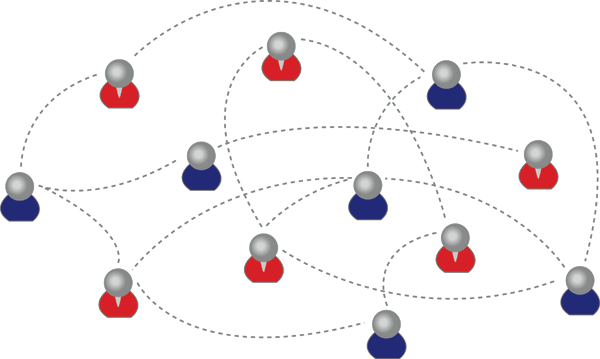
\includegraphics[width=\textwidth]{images/social-network_3.png}
			\caption{}
			\label{socialnetwork}
		\end{subfigure}
		\quad 
		\begin{subfigure}[b]{0.4\textwidth}
			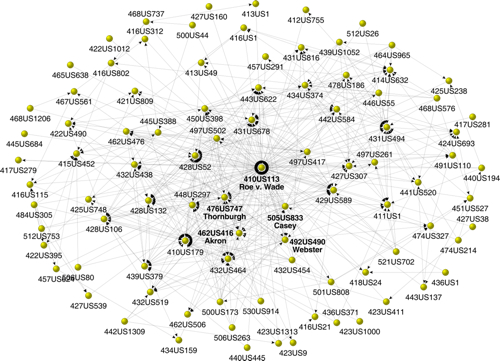
\includegraphics[width=\textwidth]{images/citation.jpg}
			\caption{}
			\label{citationntk}
		\end{subfigure}
		
		\begin{subfigure}[b]{0.4\textwidth}
			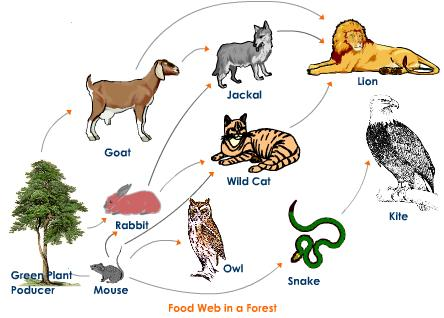
\includegraphics[width=\textwidth]{images/foodweb.jpeg}
			\caption{}
			\label{foodweb}
		\end{subfigure}
		\quad 
		\begin{subfigure}[b]{0.4\textwidth}
			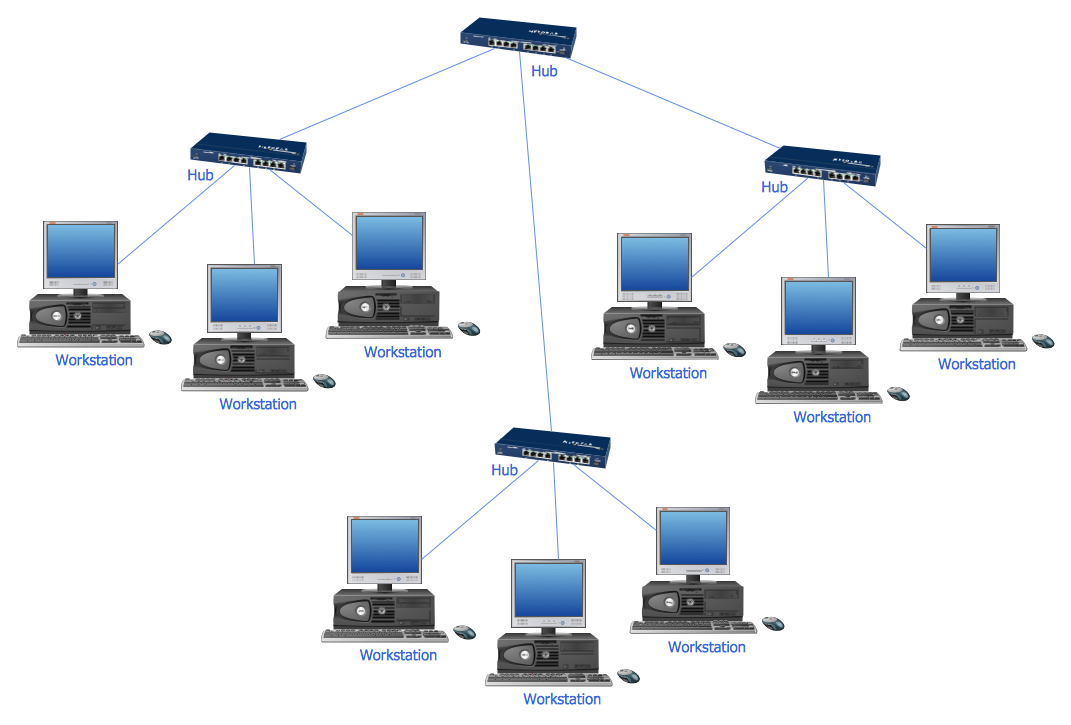
\includegraphics[width=\textwidth]{images/computer-2.png}
			\caption{}
			\label{internet}
		\end{subfigure}
		\caption{Networks in real world: (\subref{socialnetwork}) A social network. (\subref{citationntk}) A citation network. (\subref{foodweb}) A food web.  (\subref{internet}) Computer network. Source: \citep{googleimages}}
	\end{figure} 

\section{Paths and Walks}
\begin{defn}[Walk]
	A walk in a network is a series of edges (not necessarily distinct)
	\begin{eqnarray*}
		(u_1,v_1),(u_2,v_2),\ldots,(u_l,v_l), \quad \text{ for which }  v_i=u_{i+1} ~(i=1,2,\ldots,l-1).
	\end{eqnarray*}
	A walk from $v_1 $ to $v_{l+1}$ is one of length $l$ \citep{estrada2015first}.
\end{defn}

A walk of length $k$ is referred to as a $k$-walk. We can compute the number of $k$-walks between any pair of nodes in a simple undirected unweighed graph using the entries of $\mathbf{A}^k$ where $A$ is the adjacency matrix whose entries a given by
\begin{eqnarray}
A_{ij} = \begin{cases} 1 &\mbox{if } i \text{ and } j \text{ are adjacent}, \\
0 & \text{otherwise}.
\end{cases}
\end{eqnarray}


%\begin{exa}
%	Let us compute the number of $2$-walks and $3$-walks between pairs of nodes in network in Fig.~\ref{matrixgraph}.
%	\begin{eqnarray*}
%		\mathbf{A}^2 = \begin{pmatrix}
%			2 & 1 & 2 & 1 \\
%			1 & 3 & 2 & 2 \\
%			2 & 1 & 2 & 1  \\
%			1 & 2 & 1 & 3
%		\end{pmatrix}, \quad
%		\mathbf{A}^3 = \begin{pmatrix}
%			2 & 5 & 2 & 5 \\
%			5 & 4 & 5 & 5 \\
%			2 & 5 & 2 & 5 \\
%			5 & 5 & 5 & 4
%		\end{pmatrix}
%	\end{eqnarray*}
%	From the matrix $\mathbf{A}^2$, we can tell that there are $2$ walks of length $2$ between nodes $1$ and $3$, $1$ walk of length $2$ between nodes $3$ and $4$, $2$ walks of length $2$ between nodes $2$ and $4$, etc.
%	From matrix $\mathbf{A}^3$, there are $2$ walks of length $3$ between nodes $1$ and $3$, node $3$ to it self, and node $1$ to it self. There are $5$ walks of length $3$ between nodes $2$ and $3$, nodes $2$ and $4$, etc.
%	%The diagonal entries of  $\mathbf{A}^2$ are the node degrees because the only $2$-walks from a node and back to it self are the closed walks from the node to its neighbors and then back to the node which implies the total number of such $2$-walks is equal to the number of the node's neighbors.
%	%The diagonal entries of $\mathbf{A}^3$ correspond to the number of triangles a particular node is a part of.
%\end{exa}

\begin{defn}[Path]
	A path of length $l$ is a walk of length $l$ in which all the nodes and edges are distinct. A closed path is called a cycle \citep{estrada2011structure}. For any pair of nodes $v_i$,$v_j$ in a connected graph, there exists at least one path connecting $v_i$ to $v_j$. The paths with minimum length are referred as shortest-paths.
\end{defn}

\begin{defn}[Irreducible set of shortest paths]
	
	An irreducible set of shortest paths of length $l$ is the set $P_l ={P_l(v_i,v_j),P_l(v_i,v_r),\cdots, P_l(v_s,v_t)}$ in which the endpoints of every shortest-path $P_l(v_i,v_j)$ in the set are different.
	Each path in this set is referred to as an irreducible shortest-path \citep{estrada2012path}.\end{defn}

\begin{defn}[Connected component of a graph]
	A component of an undirected graph is a subgraph in which any two vertices are connected to each other by paths, and which is connected to no additional vertices in the supergraph \citep{newman2010networks}. 
	A connected component is also referred to as a maximal connected subgraph of a graph.
\end{defn}

\begin{defn}[Transition matrix of the random walk on a Graph]
	It is the $n \times n$ matrix $P_G$ whose entries are given by
	\begin{equation}
	P_{ij} = \frac{1}{d_i} A_{ij},
	\end{equation}
	In otherwords, $P_G = D_{G} ^ {-1} A$
\end{defn}

\section{Laplacian Matrix}
The Laplacian matrix is one of matrices used for representation of a network. Previously, a lot of research efforts were geared towards the study of the adjacency matrix and its spectral properties. However, it has lately been discovered that the spectral properties of a Laplacian matrix give more information pertaining the structure of the network as compared to the adjacency matrix. In this essay therefore, we study the spectrum of the Laplacian matrix of the network with the aim of obtaining information about the structure of the network. In addition, we explore the various applications of the Laplacian of a network in real-world.

The Laplacian matrix, sometimes called admittance matrix or Kirchhoff matrix, is a matrix representation of a network. The Laplacian matrix provides useful information about the properties of a network. 
It is for this reason that researchers have in studying the Laplacian matrix.

\subsection{Definitions and Properties of the Laplacian Matrix}

\begin{defn}[Laplacian Matrix]
	The Laplacian matrix of a network is the difference between the degree matrix $\mathbf{D}$ and the adjacency matrix $\mathbf{A}$ of a network. That is,
	\begin{eqnarray}
	\mathbf{L} = \mathbf{D} - \mathbf{A}.
	\end{eqnarray}
	Given a simple network $G=(V,E)$, the entries of the Laplacian matrix $\mathbf{L(G)}$  are defined as
	\begin{eqnarray}
	L_{ij} = \begin{cases} k_{v_i} &\mbox{if } i = j \\
	-1 &\mbox{if } i \neq j \text{ and } v_i \text{ is adjacent to } v_j \\
	0 & \text{otherwise},
	\end{cases}
	\end{eqnarray}
	where $k_{v_i}$  denotes the degree of node $i$ \citep{estrada2011structure}.
	
	Alternatively, we can define the Laplacian matrix of a graph in terms of the vertex-edge incidence matrix $\mathbf{B}$. That is,
	\begin{eqnarray}
	\mathbf{L} =  \mathbf{B} \mathbf{B}^T,
	\label{lintermsb}
	\end{eqnarray}
	where $\mathbf{B}^T$ is the transpose of $\mathbf{B}$ \citep{estrada2011structure}.
\end{defn}

%\begin{defn}[Normalized Laplacian matrix]
%The normalized Laplacian matrix is defined as 
%\begin{eqnarray*}
%\mathbf{\mathcal{L}} = \mathbf{D}^{-1/2} \mathbf{L} \mathbf{D}^{-1/2} = \mathbf{I} -\mathbf{D}^{-1/2} \mathbf{A} \mathbf{D}^{-1/2}
%\end{eqnarray*}
%where $\mathbf{D}^{-1/2}$ is the diagonal matrix determined by the inverse square root of each diagonal entry of the degree matrix \citep{estrada2011structure}. Then, the entries of $\mathbf{\mathcal{L}}$ are given by
%\begin{eqnarray*}
%\mathcal{L}_{ij} = \begin{cases} 1, &\mbox{if } i = j \text{ and } k_i \neq 0;\\
%-(k_ik_j)^{-1/2}, &\mbox{if } i \sim j; \\ 
%0, & \text{otherwise}.
%\end{cases}
%\end{eqnarray*}
%\end{defn}

\begin{exa} We compute the Laplacian matrix of the network in Fig.~\ref{fig:laplace-graph}.
	\begin{figure}[!h]
		\centering 
		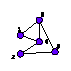
\includegraphics[width=0.24\textwidth]{images/laplace-graph.pdf}
		\caption{A Network $G$.}
		\label{fig:laplace-graph}
	\end{figure} 
	
	\begin{align*}
	\mathbf{L} = \begin{pmatrix*}[r]
	2 & 0 &-1 & -1  & 0 \\
	0 & 2 & 0 & -1 & -1 \\
	-1 & 0 &  3 & -1 & -1  \\
	-1 & -1 & -1 & 3 & 0 \\
	0 & -1 & -1 & 0 &  2
	\end{pmatrix*}.
	\end{align*}
	
	%\begin{minipage}{.25\textwidth}
	% align*}
	%  \mathb \centering 
	%   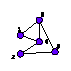
\includegraphics[width=\textwidth]{images/laplace-graph.pdf}
	%  \captionof{figure}{A Network $G$.}
	%  \label{fig:laplace-graph}
	%\end{minipage} \qquad \qquad
	%\begin{minipage}{.23\textwidth}
	%\begin{f{L} = \begin{pmatrix*}[r]
	%  2 & 0 &-1 & -1  & 0 \\
	%  0 & 2 & 0 & -1 & -1 \\
	%  -1 & 0 &  3 & -1 & -1  \\
	%  -1 & -1 & -1 & 3 & 0 \\
	%  0 & -1 & -1 & 0 &  2
	%  \end{pmatrix*}.
	%\end{align*}
	%\end{minipage}
	% ~
	%\begin{minipage}{.23\textwidth}
	%\begin{align*}
	%\renewcommand*{\arraystretch}{1.2}
	%  \mathcal{L} = \begin{pmatrix*}[r]
	%  1 & 0 &-\frac{1}{\sqrt{6}} & -\frac{1}{\sqrt{6}} & 0 \\
	%  0 & 1 & 0 & -\frac{1}{\sqrt{6}} & -\frac{1}{2}\\
	%  -\frac{1}{\sqrt{6}} & 0 &  1 & -\frac{1}{3} & -\frac{1}{\sqrt{6}}  \\
	%  -\frac{1}{\sqrt{6}} & -\frac{1}{\sqrt{6}} & -\frac{1}{3}& 1 & 0 \\
	%  0 & -\frac{1}{2} & -\frac{1}{\sqrt{6}} & 0 &  1
	%  \end{pmatrix*}.
	%\end{align*}
	%\end{minipage}
	\label{example:laplace}
\end{exa}

The properties of the Laplacian matrix of a network are very useful in understanding the structure of a network. We therefore discuss some of these properties.
\begin{enumerate}	
\item{Real and symmetric matrix} 

The entries of the Laplacian matrix are real numbers and are symmetric with respect to the main diagonal \citep{das2004laplacian}. Thus, the spectrum is real.
\item{Singular matrix}

The Laplacian matrix is a square matrix that is not invertible. Its determinant is equal to zero \citep{das2004laplacian}.
\item{Positive semi-definite}

A matrix is positive semi-definite if and only if all its eigenvalues are non-negative. For a given matrix $L$, this property is denoted by $A\geq 0$. 

Suppose the eigenvalues of a Laplacian matrix are: $\lambda_1,\lambda_2,\ldots, \lambda_n$, we show that $\lambda_i \geq 0 ~\forall~i$.
\begin{proof}
	Let $\mathbf{v}_i$ be a normalised eigenvector of $\mathbf{L}$ with eigenvalue $\lambda_i$. Then, using Equation (\ref{lintermsb})
	\begin{eqnarray*}
		\mathbf{v}_i^T \mathbf{B}^T \mathbf{B} \mathbf{v} &=& \mathbf{v}_i^T \mathbf{L} \mathbf{v}_i = \lambda_i  \mathbf{v}_i^T \mathbf{v}_i  = \lambda_i.
	\end{eqnarray*}  
	Thus, any eigenvalue $\lambda_i$ of the Laplacian matrix is equal 
	to $(\mathbf{v}_i^T \mathbf{B}^T \mathbf{B} \mathbf{v}_i)$ which can be written as $(\mathbf{v}_i \mathbf{B})^T (\mathbf{B} \mathbf{v}_i)$. The quantity $(\mathbf{v}_i \mathbf{B})^T (\mathbf{B} \mathbf{v}_i)$  is the inner product of a real vector $(\mathbf{B} \mathbf{v}_i)$ with itself, that is, the sum of the squares of the real elements of the vector $(\mathbf{B} \mathbf{v}_i)$ and hence it is non-negative \citep{estrada2015first}.
\end{proof}

\end{enumerate}
\subsection{Spectrum of the Laplacian Matrix}
The spectrum of the Laplacian provides useful information about the structure of a network. The spectrum of the Laplacian matrix is the set of all its eigenvalues and their multiplicities \citep{estrada2011structure}. Let $\lambda_1 < \lambda_2 < \ldots < \lambda_n$ be the distinct eigenvalues of $\mathbf{L}$ and let $m(\lambda_1),m(\lambda_2), \ldots,m(\lambda_n)$ be their multiplicities. Then, the spectrum of $\mathbf{L}$ is written as
\begin{eqnarray}
Sp\mathbf{L} = 
\renewcommand*{\arraystretch}{1.1}
\begin{pmatrix*}
\lambda_1 & \lambda_2 & \ldots & \lambda_n \\
m(\lambda_1) & m(\lambda_2) & \ldots & m(\lambda_n)
\end{pmatrix*}.
\end{eqnarray}

Let us write the eigenvalues of $\mathbf{L}$ in decreasing order: $\lambda_n  \geq \lambda_{n-1} \geq  \cdots \geq \lambda_2 \geq \lambda_1 =0 $. Some of the results associated with the spectrum of the Laplacian matrix include:
\begin{itemize}
	\item The eigenvalues of $\mathbf{L}$ are bounded as 
	$ 0 \leq \lambda_j \leq 2k_{max} \quad \text{and} \quad \lambda_n \geq k_{max} $.
	\item The eigenvalue $\lambda_1$ is always equal to zero \citep{estrada2011structure}. Atleast one eigenvalue of the Laplacian is $0$.
	\begin{proof}
		Consider the vector $v= (1/\sqrt{n}, \cdots, 1/\sqrt{n}) $. We know that the $i$th entry of $Lv$ is 
		
		$\sum_{i\sim j} v_{(i)}- v_{(j)} = \sum_{i\sim j} (1/\sqrt{n} - 1/\sqrt{n}) = 0 = 0 \cdot v_{(i)}$.
	\end{proof}
	%\item The smallest non-zero eigenvalue of $\mathbf{L}$ is called the spectral gap.
	\item The multiplicity of $0$ as an eigenvalue of $\mathbf{L}$ is equal to the number of connected components in the network \citep{estrada2011structure}.
	\item Every row sum and column sum of $\mathbf{L}$ is zero. Thus, the vector $\mathbf{v_1}$ of all ones is an eigenvector associated with $\lambda_1 =0$, since $\mathbf{Lv_1} = \mathbf{0} $ \citep{das2004laplacian}.
	\item  A network is connected if its second smallest eigenvalue is nonzero. That is, $\lambda_2> 0$ if and only if $G$ is connected. The eigenvalue $\lambda_2$ is thus called the algebraic connectivity of a network, $a(G)$. The magnitude of this value depict how well connected  the over all graph is. The algebraic connected significant implications for properties such as clustering and synchronizability.
	The eigenvector corresponding to the eigenvalue $\lambda_2$ is called the Fiedler vector \citep{estrada2015first}.
	
	\item Let $G$ be a graph with connected components $G_i (1 \leq i \leq s)$. Then the spectrum of $G$ is the union of the spectra of $G_i$ (and multiplicities are added) \citep{brouwer2011spectra}.
	
	\item For a graph $G$, the sum of the eigenvalues, that is, the trace of $L$ is twice the number of edges of $G$. Mathematically, $\sum_{i=1}^n \lambda_i = Tr(L) = 2E.$\\
	
\end{itemize}


\begin{thm}[Fiedler, 1975]
	Suppose $G = (V,E)$ is a connected network with graph Laplacian $\mathbf{L}$ whose second smallest eigenvalue is $\lambda_2 > 0$. Let $x$ be the eigenvector associated with $\lambda_2$. Let $r \in \mathbb{R}$ and partition the nodes in $V$ into two sets
	\begin{eqnarray}
	V_1 = \{i \in V|x_i \geq r\}, ~ V_2 = \{i \in V | x_i < r\}, 
	\end{eqnarray}
	then the subgraphs of $G$ induced by the sets $V_1$ and $V_2$ are connected \citep{estrada2015first}.
	\label{fiedler}
\end{thm}
This result is useful for partitioning a network while ensuring that all the parts remain connected. This method of partitioning using eigenvalues is known as spectral clustering. For clusters of equal size, we choose $r$ such that it is the median value of $x$. 

\begin{exa} Using Theorem \ref{fiedler}, let us partition the network in Fig.~\ref{clusters}(\subref{whole-graph}) into two clusters. First, we compute the eigenvalues and corresponding eigenvectors of the Laplacian matrix $\mathbf{L}$ of the network which are: $\lambda_1=0,\lambda_2=2,\lambda_3=4,\lambda_4=4$. The second smallest non-zero eigenvalue $\lambda_2=2$ is associated with eigenvector $ \mathbf{v_2}=(1,0,0,-1)^T$ which implies that $x_1 =1, x_2 = 0, x_3=0$ and $x_4=-1$. Taking $r=0$, we obtain the two vertex sets $V_1$ and $V_2$ as $V_1 = \{1,2,3 \}$ and $V_2 =\{4 \}$. The two clusters are shown in Fig.~\ref{clusters}(\subref{cluster-graph}).
	
	\begin{figure}[!h]
		\centering
		\begin{subfigure}[b]{0.21\textwidth}
			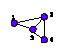
\includegraphics[width=\textwidth]{images/cluster-graph.pdf}
			\caption{}
			\label{whole-graph}
		\end{subfigure}
		\begin{subfigure}[b]{0.28\textwidth}
			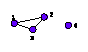
\includegraphics[width=\textwidth]{images/partitions-graph.pdf}
			\caption{}
			\label{cluster-graph}
		\end{subfigure} 
		\caption{(\subref{whole-graph}) A network (\subref{cluster-graph}) and its two clusters of size $3$ and $1$.} \label{clusters}
	\end{figure}
\end{exa}

Some analytic expressions for the spectra of different kinds of simple networks are:
\begin{itemize}
	\item Star, $S_n$ : $Sp(\mathbf{L}) = \{ 0~ 1^{n-2}~n\}$. 
	
	\item Complete, $K_n$ : $Sp(\mathbf{L}) = \{ 0~ n^{n-1} \}$. 
	
	\item Complete bipartite, $K_{m,n}$ : $Sp(\mathbf{L}) =\{ 0 ~ m^{n-1} ~ n^{m-1}\}$.
	
\end{itemize}

\begin{thm}[Kirchoff's Matrix-Tree Theorem]
	If $G$ is a connected graph with Laplacian matrix $\mathbf{L}$, then the number of unique spanning trees of $G$ is equal to the value of any cofactor of the matrix $\mathbf{L}$ \citep{harris2008combinatorics}.
	\label{thm:kirchoff}
\end{thm}
%For a given connected graph $G$ with $n$ vertices, let $\lambda_1, \lambda_2, \ldots, \lambda_{n-1}$ be the non-zero eigenvalues of its Laplacian matrix. Then the number of spanning trees of $G$ is
%\begin{eqnarray}
%t(G) = \frac{1}{n} \lambda_1 \lambda_2 \ldots \lambda_{n-1}.
%\label{spanning}
%\end{eqnarray}

\begin{exa} Let us compute the number of spanning trees of network $G$ in Fig.~\ref{clusters}(\subref{whole-graph}) using Theorem \ref{thm:kirchoff}.
	The $(i,j)$ cofactor is obtained as $(-1)^{i+j} \times |\mathbf{L}(i|j)|$ where $\mathbf{L}(i|j)$ is the $(n-1) \times (n-1)$ submatrix of $\mathbf{L(G)}$ obtained by deleting its $i$th row and $j$th column. The Laplace matrix is given by
	\begin{eqnarray*}
		\mathbf{L(G)} = \begin{pmatrix*}[r]
			2 & -1 & -1  & 0 \\
			-1 & 3 & -1 & -1  \\
			-1 & -1 & 3 & -1 \\
			0 & -1 & -1 &  2
		\end{pmatrix*},\text{ deleting row $1$ and column $1$ gives } \mathbf{L}(1|1) = \begin{pmatrix*}[r]
			3 & -1 & -1 \\
			-1 & 3 & -1  \\
			-1 & -1 & 2 
		\end{pmatrix*}.
	\end{eqnarray*}
	The $(1,1)$ cofactor of $\mathbf{L(G)}$ is $ (-1)^2 \times |\mathbf{L}(1|1)| = 8$. Thus, there are $8$ spanning trees of graph $G$.
	%Using Equation (\ref{spanning}), we have $\lambda_4=0,\lambda_3=2,\lambda_2=4,\lambda_1=4$, and $n=4$. Thus,
	%\begin{eqnarray*}
	%t(G) = \frac{1}{4} ( 4  \times 4 \times 2 ) = 8.
	%\end{eqnarray*}
\end{exa}

%\begin{figure}[!h]
%    \centering
%        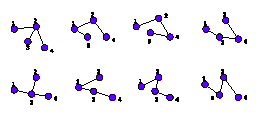
\includegraphics[width=0.7\textwidth]{images/spanningtreestotal.pdf}
%      \caption{ The $8$ unique spanning trees of graph in Fig.~\ref{clusters}(\subref{whole-graph}).}
%      \label{all-spanning}
%\end{figure}
	
\section{Robustness of Complex Systems}
	A complex systems is considered robust if it can with stand failures or perturbations that is to say a system can still perform as expected even in circumstances of failure of one or more components in the system. 
	In other words, robustness intuitively deals with the existence of back-up possibilities. In a network, this cab be captured in the existence of alternative paths with in the network.
	 Robustness of systems plays an important role in a number of fields for instance in Engineering, understanding robustness acts as a basis for designing communication, transportation systems, power grids that can perform basic operation despite failure of some system components. In biology,robustness explains why some mutations lead to diseases while others do not. For ecologists and environmental experts, robustness helps in predicting the failure of an ecosystem when faced with disruptive human behaviours. In general, study of system robustness aids in understanding system operation, improving system performance and designing of new robust systems. 
	As mentioned earlier, the study of a network or graph underlying a complex system provides insights about the properties and characteristics of that systems. Thus, Barabasi \citep{barabasi2016network} highlighted the fact that networks play a vital role in robustness of complex systems which implies that exploring robustness of the network reflects that of the system.
	 
	\subsection{Robustness measures in networks}
	According to Ellens \citep{ellens2013graph}, robustness of a network is its ability to perform well when subject to failures or attacks. The attacks take on two forms namely: random attacks and targeted attacks. However, in order to tell whether a particular network is robust, there is need for a measure that quantifies the robustness. In the past, various robustness measures have been put forward by researchers \citep{sydney2008elasticity}. We explore some of the common measures of robustness in networks. We categorise the measures as follows:
	\subsubsection{Connectivity-based measures}
	Here we consider robustness measures that are based on the connectivity of the network. These include the classical connectivity $\kappa$, edge connectivity $\kappa_e$, and vertex connectivity $\kappa_v$. Firstly, the classical connectivity $\kappa$ is a measure whose value $\kappa=1$ for graphs in which there is a path between any pair of vertices that is connected graphs and $\kappa=0$ for unconnected graphs that is graphs in which atleast one pair of vertices  for which no path exists between them. Secondly, the edge connectivity $\kappa_e$ and vertex connectivity $\kappa_v$ are respectively the minimum number edges and vertices that need to be removed to disconnect the graph. The inequality $\kappa_v \leq \kappa_e \leq \delta_{min}$ holds for non-complete graphs, where $\delta_{min}$ is the minimum degree of vertices in a graph.
	\subsubsection{Distance-based measures}
	\begin{enumerate}
		\item Diameter
	
		The diameter of a graph, denoted as $D$, is the maximum distance between pairs of nodes in the graph\citep{wang2003complex}. The diameter of a graph $G= (V,E )$ is defined as \[ D = \max_{i,j \in V} \{d_{ij}\},\] where $d_{ij}$ is the shortest path between node $i$ and $j$. Based on the diameter, a graph is considered more robust if it's diameter is shorter.
		\item Average Path Length
		
		The average path length of a network is the average number of steps along the shortest paths for all possible pairs of network nodes. Let $G = (V , E )$ be a graph the average path length $L_G$ is defined by
		\begin{eqnarray}
		L_G = \frac{1}{n(n-1)} \sum_{i,j \in V,~i \neq j} d_{ij},
		\end{eqnarray}
		where $d_{ij}$ is the shortest path between node $i$ and $j$ and $n$ is the total number of nodes in $G$ \citep{wang2003complex}. 
		On comparing the average path length and diameter as measures of robustness, the former is considered a better measure as it strictly decreases on addition of edges which is not necessarily the case with the latter.
		\item Efficiency
		
		We can observe that we cannot compute the robustness of disconnected graph based on the two distance-based measures discussed previously. However, this is a possibility when we adopt the efficiency measure. 
		The efficiency of a graph, $E$ is defined as
		\begin{eqnarray}
			E =\frac{1}{n(n-1)} \sum_{i,j \in V,i\neq j} \frac{1}{d_{ij}}.
			\label{eqn:eff}
		\end{eqnarray}
		It is important to note that these measures based on distance consider only shortest path distances which implies that other alternative paths are not put into consideration which is a disadvantage for that matter.
	\end{enumerate}
	
	\subsection{Reliability Polynomial}
	
	\subsection{Spectral Graph measures}
	\begin{enumerate}
		\item Algebraic connectivity
		
		Given the spectrum of the Laplacian matrix of a graph $G$ in which the eignvalues are arranged in non-decreasing order: $0=\lambda_1\leq \lambda_2 \leq \cdots \leq \lambda_n$. The algebraic connectivity is the second smallest eigenvalue $\lambda_2$ of the Laplacian. It is the most common measure of robustness.The algebraic connectivity is equal to zero if and only if the graph is unconnected. The disadvantage of this measure is the fact that it does not necessarily capture the addition of edges to a graph that is to say the value of $\lambda_2$ does not strictly increase on edge addition.
		\item Number of spanning trees
				
		A spanning tree is a subgraph containing $n-1$ edges and no cycles. According to the Kirchoff's Matrix-Tree Theorem, the number of unique spanning trees,$\xi$ of graph $G$ is equal to the value of any cofactor of the Laplacian \citep{harris2008combinatorics}. It  is given by
		\begin{equation}
		\xi = \frac{1}{n} \prod_{i=2}^{n} \lambda_i.
		\end{equation}
		Baras and Hovareshti suggest the number of spanning trees as a global indicator of network robustness to edge removal. It has been proved that for $p$ close to zero, the number of spanning tree gives similar results for robustness as the reliability polynomial \citep{baras2009efficient}.
		\item Effective resistance
		
		The effective graph resistance $R$, also called total effective resistance or Kirchhoff index, is
		defined as the sum of the effective resistances over all pairs of vertices. It can be expressed in terms of the non-zero eigenvalues of Laplacian as
		\begin{equation}
		R = \sum_{1\leq i < j \leq n} R_{i,j} = n \sum_{i=2}^{n} \frac{1}{\lambda_i}
		\end{equation}
		Unlike the algebraic connectivity, the effective resistance involves not only one but all the non-zero eigenvalues of the Laplacian. It is for this result that any changes due to edge addition or removal are captured which makes the latter a better measure of robustness.
		\item Natural Connectivity
		
		This spectral measure of robustness was put forward by Wu et al.\citep{wu2564spectral}. It captures the core of robustness that is the capturing of redundancy of alternative paths. This is achieved by quantifying the weighted number of walks of all lengths in the graph. Closed walks are related to subgraphs of a graph for instance a closed walk of length $k=3$ represents a triangle. The number of closed walks of all lengths is obtained following the principle used in the computing the subgraph centrality as in \citep{estrada2011structure} in which the shorter closed walks have more influence than their longer counterparts. The penalisation entails dividing the sum of closed walks of length $k$ by the factorial of $k$. That is,  
		\begin{equation}
		S = \sum_{k=0}^{\infty} \frac{n_k}{k!},
		\label{sumclosed}
		\end{equation} 
		where $n_k$ is the number of closed walks of length $k$. We also know that,
		\begin{equation}
		n_k = trace(\mathbf{A}^k) = \sum_{i=1}^{N} \lambda_{i} ^k,
		\end{equation}
		where $\lambda_i$ is the $i$th largest eigenvalue of $\mathbf{A}(G)$.
		Substituting for $n_k$ in Eqn.\ref{sumclosed} gives
		\begin{equation}
		S = \sum_{k=0}^{\infty} \sum_{i=1}^{N} \frac{\lambda_{i} ^k} {k!} =  \sum_{i=1}^{N}\sum_{k=0}^{\infty} \frac{\lambda_{i} ^k} {k!}= \sum_{i=1}^{N} e^{\lambda_i}.
		\label{sumexpn}
		\end{equation}
		From Eqn. \ref{sumexpn}, we observe two facts. First, the weighted sum of closed walks can be obtained from the spectrum of the Adjacency matrix of a graph. second, the sum $S$ will be a large number for large $N$ and  thus the need to scale $S$. The scaled version of $S$, termed as the 'average eigenvalue' and denoted by $\bar{\lambda}$  is given by
		\begin{equation}
		\bar{\lambda} = \ln \big( \frac{S}{N}\big) = \ln \Big( \frac{\sum_{i=1}^{N} e^{\lambda_i}}{N} \Big).
		\end{equation}
		Unlike the algebraic connectivity, the natural connectivity changes monotonically when edges are added or deleted which is one of the desired properties of a robustness measure.
	\end{enumerate}
	\section{Principal Component Analysis}
	
    \section{Diffusion on networks}
    Diffusion is, among others, the movement of substance from a region of high concentration to a region of low concentration. Such substance include heat, gas, etc. \citep{newman2010networks}.
    
    Diffusion process over networks is one of the methods used in developing simple models that depict the spread of infections in a population, dissemination of information over social network for instance social network marketing, spread of heat over a conductor, among others. A number of models based on diffusion process have been developed and documented in \citep{estrada2011epidemic,kasprzak2012diffusion,lopez2008diffusion}.
    
    \subsection{Heat Diffusion Models}
    In this work, we consider spread of heat on a network. Recently, various models have been developed to depict the spread of heat heat diffusion process on networks which include selection of marketing candidates in social network marketing, data analysis and processing in which the observed data is considered as a sum of diffusion processes, dimensionality reduction and classification problems   \citep{ma2008mining,thanou2017learning,belkin2003laplacian}.
    
    Let $G=(V,E)$ be a simple connected undirected graph with vertex set $V$ and edge set $E$. Suppose we randomly select a few nodes ( that is, sources) to which we assign specific amounts of heat as in vector $\phi_0$. With the heat diffusion coefficient, $\varepsilon \in [0,1]$ which controls the rate of diffusion. When $C$ tends to $0$, heat transfer among nodes becomes difficult and as a result, heat does not spread to each of the nodes with in the network. However, as $C$ tends to $1$, heat spreads rapidly among nodes and thus, with out loss, heat is distributed to all nodes in the network.
    
   At each time $t$, we obtain the quantities of heat at each node, $\phi_t$. The spread of heat is considered to occur following the edges connecting nodes, that is to say, through direct interactions.  
%     We then try to understand how the heat will spread through out the network, whether equilibrium can be attained and if so, when does this happens?? We then explore the impact of network structure and node centralities on heat diffusion.
%    \begin{enumerate}[a)]
%    	\item Direct interactions
%    	Let us consider a simple network where a few randomly selected nodes are assigned quantities of heat $\phi_i$. The diffusion process is considered to occur by means of interactions between neighbouring nodes in the network. This mode of interaction is referred to as direct interactions. 
    	
    	The process of heat spread through out the network can therefore be modelled by
    	\begin{equation}
    	\frac{d\phi_i}{dt} = \varepsilon \sum_j (\mathbf{A}_{ij} - \delta_{ij} k_i) \phi_j,
    	\label{difusion}
    	\end{equation}
    	where $\mathbf{A}$ is the adjacency matrix, $k_i$ is the degree of node $i$, and $\delta_{ij}$ is the Kronecker delta whose value is $1$ if $i=j$ and $0$ otherwise. In matrix-vector notation, we have
    	\begin{equation}
    	\frac{d\boldsymbol{\phi}}{dt} = -\varepsilon\mathbf{L}\boldsymbol{\phi}, \quad \boldsymbol{\phi}(0) = \boldsymbol{\phi}_0 ,
    	\label{dif-final-eqn}
    	\end{equation}
    	whose solution is 
    	\begin{eqnarray}
    	\boldsymbol{\phi}(t) = \boldsymbol{\phi}_0~e^{-\varepsilon\mathbf{L}t}.
    	\end{eqnarray}
    	Alternatively, the solution can be expressed as a linear combination of eigenvectors of the Laplacian matrix. That is
    	 \begin{eqnarray*}
    	 	\boldsymbol{\phi}(t) = \sum_i \langle \boldsymbol{\phi}(0),\mathbf{v}_i \rangle \quad e^{-\varepsilon\lambda_i t} \mathbf{v}_i,  
    	 \end{eqnarray*}
    	 where $\lambda_i$, $\mathbf{v}_i$ are respectively the eigenvalues and corresponding eigenvectors of the Laplacian matrix and $\langle \boldsymbol{\phi}(0),\mathbf{v}_i \rangle$ is simply the projection of $\boldsymbol{\phi}(0)$ onto the set of eigenvectors.
    	 
    	 \subsection{ Equilibrium behaviour }
    	 As $t$ goes to infinity, we have 
    	 \begin{equation}
    	 \lim_{t \to \infty} e^{-\varepsilon\lambda_i t} = \begin{cases} 0 &\mbox{if } \lambda_i > 0 \\
    	 1 & \mbox{if } \lambda_i = 0, \end{cases} 
    	 \end{equation}
    	 Asymptotically, the equilibrium state is completely determined by the kernel of $\mathbf{L}$. Since $\sum_{j} \mathbf{L}_{ij}=0$, it is easy to see that $\mathbf{v^1}= \frac{1}{\sqrt{n}}[1,\cdots,1]$, the eigenvector associated with $\lambda_i =0$, is in the kernel of $\mathbf{L}$. We then have
    	 %$\displaystyle \lim_{t \to \infty}\boldsymbol{\phi}(t)$, $a_i(t) = a_i(0) e^{-C \lambda_i t}$ where $\lambda_i = 0$. Since $L(\mathbf{v^1}) = \mathbf{0}$, for a given initial condition $\mathbf{a}(0)$ for a network with $n$ nodes, we have
    	 \begin{equation}
    	 \lim_{t \to \infty}\boldsymbol{\phi}(t) = \langle \boldsymbol{\phi}(0), \mathbf{v^1} \rangle \mathbf{v^1}.
    	 \end{equation}
    	 The quantity of heat $\phi_j(t)$ at any node $j$ at time $t$ is given by
    	 \begin{equation}
    	 \lim_{t \to \infty}\phi_j(t) = \frac{1}{n} \sum_{i = 1}^n \phi_i(0). 
    	 \end{equation}
    	 At steady state, the value of $\boldsymbol{\phi}$ converges to the same value at each of the nodes in the network, which is the average of the initial values at all of the nodes. This is because, as expected, neighboring nodes in the network will exchange heat until all nodes attain equal amounts of heat.
    	 
    	 For better understanding of the heat diffusion model, let us consider the following simple example.
    	 
    	 \begin{exa} Let us consider diffusion of heat over the network in Fig.~\ref{graph-plot}(\subref{difn-graph}). Suppose the quantity of heat at each node at time $t=0$ is given by the vector $\boldsymbol{\phi}(0)= [0.3,0.0,0.8,0.0,0.5,0.2,0.0,0.0,0.0,0.2]$, random values between $0$ and $1$. Let $\varepsilon=0.05$. Fig.~\ref{graph-plot}(\subref{difn-plot}) illustrates how heat spreads over the network in Fig.~\ref{graph-plot}(\subref{difn-graph}). 
    	 	
    	 	\begin{figure}[H]
    	 		\centering
    	 		\begin{subfigure}[b]{0.29\textwidth}
    	 			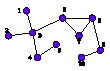
\includegraphics[width=\textwidth]{images/diffusion-graph.pdf}
    	 			\caption{}
    	 			\label{difn-graph}
    	 		\end{subfigure}~
    	 		\begin{subfigure}[b]{0.45\textwidth}
    	 			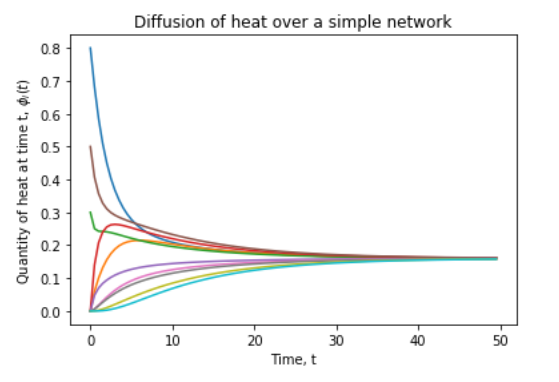
\includegraphics[width= \textwidth]{images/Diffusion-on-network-new.png}
    	 			\caption{}
    	 			\label{difn-plot}
    	 		\end{subfigure}
    	 		\caption{(\subref{difn-plot}) is an illustration of the diffusion process over the network in (\subref{difn-graph}). }
    	 		\label{graph-plot}
    	 	\end{figure}
     	  From Fig.\ref{graph-plot},we observe that at each time step $t$, nodes that initially have high amounts of heat (i.e $1,3,5,6,$ and $10$) exchange heat with adjacent nodes that initially had none or little amounts of heat. The latter gain heat from the former and eventually all nodes in the network have relatively equal amounts of heat. This explains the fact that as time $t$ increases, the quantity of heat $\boldsymbol{\phi}_j(t)$ at each node tends to the equilibrium value of $0.2$ which is attained at $t=35$. 
    	 \end{exa}
     
     \section{Impact of Structure on the rate of diffusion}
     The structure of a network basically means the way in which nodes are connected in the network. For instance, in a regular network each node is connected to equal number of nodes, for a star network one node is positioned in a way that all other nodes are connected to it.
     Let us consider two structures of networks that manifest in many artificial and real world networks.  First, the Erdos-Renyi (ER) network in which a pair of nodes is connected by random probability, $p$. The degree of nodes in ER network follow a Poisson distribution \cite{erdos1960evolution}. Second, we consider the Barabasi-Albert(BA) network in which connection of nodes follows scale free power-law distribution, that is to say, the probability of finding a node with degree $k$ decreases as the negative power of $k$. It therefore less likely to find a node with high degree (hub) compared to low degrees \cite{barabasi1999emergence, estrada2011structure} . 
     Consider ER and BA networks with $n=100$ and average degree $\bar{k}= 6$, we randomly assign quantities(range of 0 to 20) of heat to each node and allow diffusion to occur at different values of conductance $x$. After every time step $t$,we compute the quantities at each node as depicted in Figure \ref{barabasi-Erdos-compare}.
     
     %\newpage
     \begin{figure}[H]
     	\centering
     	\begin{subfigure}[b]{0.45\textwidth}
     		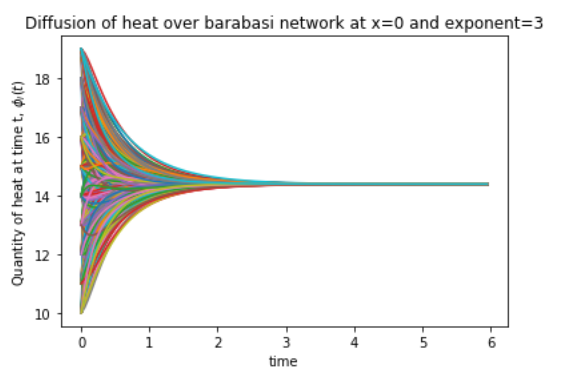
\includegraphics[width=\textwidth]{images/barabasi-x0.png}
     		\caption{$x=0$}
     		\label{barabasi-x0}
     	\end{subfigure}~
     	\begin{subfigure}[b]{0.45\textwidth}
     		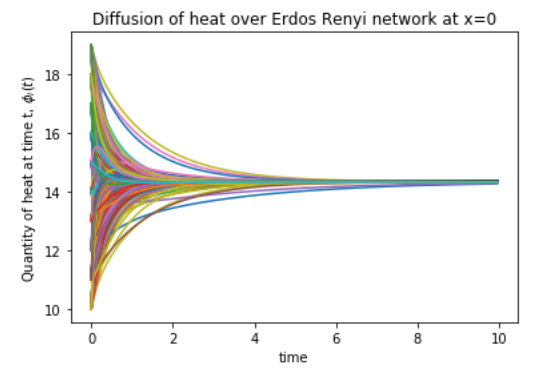
\includegraphics[width= \textwidth]{images/erdos-x0.png}
     		\caption{$x=0$}
     		\label{erdos-x01}
     	\end{subfigure}\\
     	\begin{subfigure}[b]{0.45\textwidth}
     		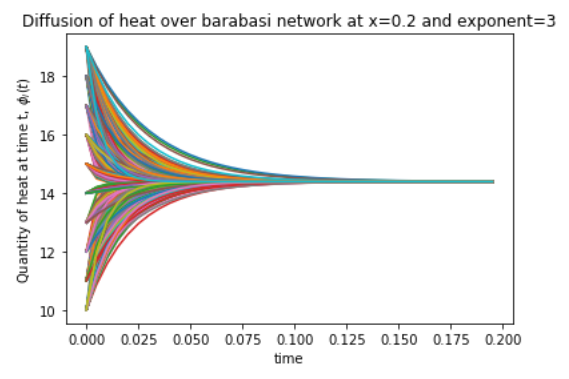
\includegraphics[width= \textwidth]{images/barabasi-x02.png}
     		\caption{$x=0.2$}
     		\label{barabasi-x02}
     	\end{subfigure}~
     	\begin{subfigure}[b]{0.45\textwidth}
     		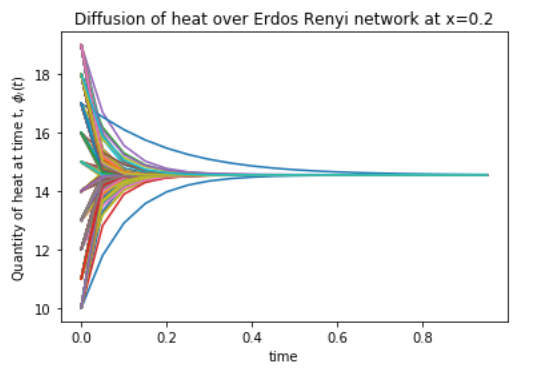
\includegraphics[width= \textwidth]{images/erdos-x02.png}
     		\caption{$x=0.2$}
     		\label{erdos-x02}
     	\end{subfigure}\\
     	\begin{subfigure}[b]{0.45\textwidth}
     		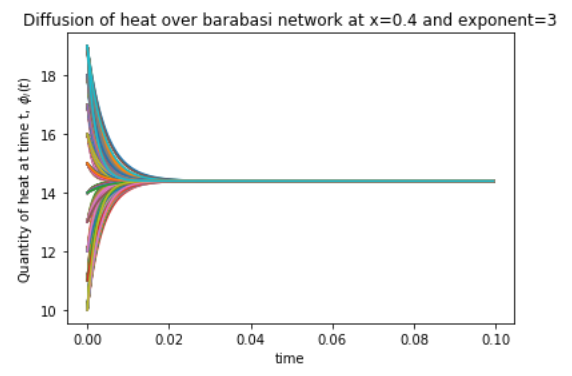
\includegraphics[width= \textwidth]{images/barabasi-x04.png}
     		\caption{$x=0.4$}
     		\label{barabasi-x04}
     	\end{subfigure}~
     	\begin{subfigure}[b]{0.45\textwidth}
     		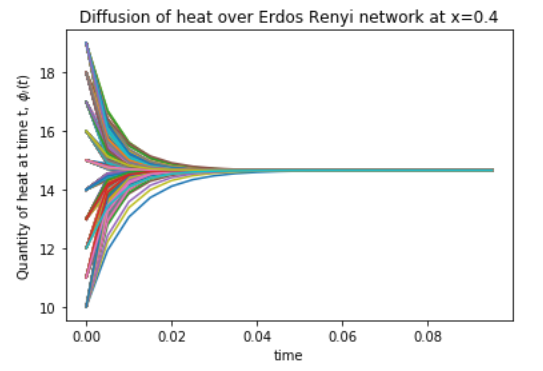
\includegraphics[width= \textwidth]{images/erdos-x04.png}
     		\caption{$x=0.4$}
     		\label{erdos-x04}
     	\end{subfigure}
     	\caption{Barabasi networks (left) and Erdos Renyi networks(right) of 1000 nodes and average degree of 6. Top row is illustration of diffusion process at $x=0$ ( i.e accounting for direct interactions only), middle row corresponds to $x=0.2$ followed by $x=0.4$ in the last row}
     	\label{barabasi-Erdos-compare}
     \end{figure}
     
     From Fig \ref{barabasi-Erdos-compare} at the top row, we observe that at $x=0$, equilibrium is reached faster for Barabasi-Alberto(BA) network ( that is after about $4$ time steps) compared to Erdos-Renyi(ER) network in which equilibrium is reached after about $10$ time steps. This is explained based on the fact that in BA networks there are more hubs compared to ER networks. These hubs tend to interact with a number of nodes with in the network thus fastening the diffusion process. On increasing $x$ to $0.2$, we observe a drastic drop in equilibrium time from  $4$ to $0.15$ time steps and from $10$ to $0.8$ time steps for BA and ER networks respectively. It is important to note that drop in equilibrium time is relatively higher in ER than in BA and this is because of the few hubs in ER networks which aids a larger number of long range interactions than in BA networks. As $x$ increases further to $0.4$, equilibrium time further drops to $0.03$ and $0.06$ for BA and ER networks respectively.
     
     \section{Influence of Heterogeneity on Diffusion over network}
     The heterogeneity of a network is the irregularity characterised by the existence of a nodes with degree significantly larger than the average degree of the network \cite{estrada2010quantifying,albert2002statistical,newman2003structure}.
     The quantification of heterogeneity is one the areas where tremendous research has been on going and various measures have been introduced \cite{estrada2010quantifying}.
     Here, we consider heterogeneity in scale free networks with $n=1000$ and average degree $\bar{k}=20$ by varying power exponent, $\gamma$. For different conductances $x$, we assign initial quantities of heat to each of the $200$ nodes with highest degree. Figure \ref{quantity-exponents} illustrates how the average quantities of heat of the selected initial diffusion nodes varies with time.
     \begin{figure}[!h]
     	\centering
     	\begin{subfigure}[b]{0.32\textwidth}
     		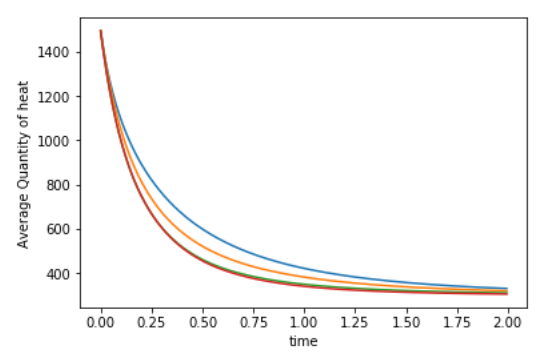
\includegraphics[width=\textwidth]{images/quantity-time-exponents-x0.png}
     		%\caption{$x=0.1, t=0$}
     		%\label{gridt0x01}
     	\end{subfigure}~
     	\begin{subfigure}[b]{0.32\textwidth}
     		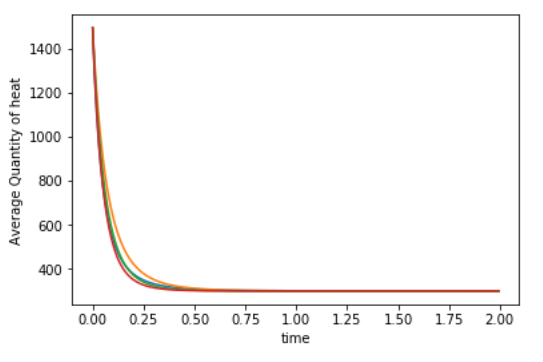
\includegraphics[width= \textwidth]{images/quantity-time-exponents-x01.png}
     		%\caption{$x=0.1, t=0.5$}
     		%\label{gridt05x01}
     	\end{subfigure}~
     	\begin{subfigure}[b]{0.32\textwidth}
     		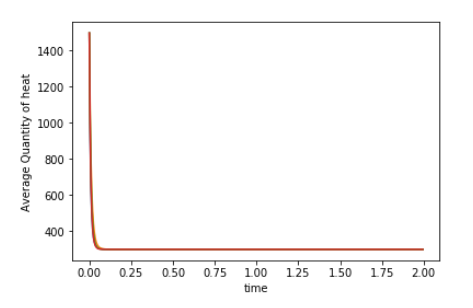
\includegraphics[width= \textwidth]{images/quantity-time-exponents-x03.png}
     		%\caption{$x=0.1, t=3.0$}
     		%\label{gridt3x01}
     	\end{subfigure} \\
     	\begin{subfigure}[b]{0.80\textwidth}
     		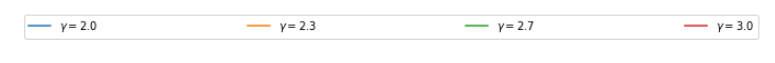
\includegraphics[width= \textwidth]{images/legend-gamma.png}
     	\end{subfigure}
     	\caption{Plots of the average quantity of heat for $200$ nodes with the highest degree centrality against time for $3$ scale free networks having different values of the power exponent($2.0$,$2.3$,$2.7$, and $3.0$), n=1000 and average degree=$6$. The figures to the left, centre and right correspond to x values $0$,$0.1$, and $0.3$ respectively.}
     	\label{quantity-exponents}
     \end{figure}
 
     \section{Impact of choice of Initial diffusion nodes on the diffusion process on networks}
     %We take a Barabasi-Albert network and Erdos-Renyi network, both of 100 nodes and average of 6. We choose $5$ nodes with the highest degree centrality to which we assign specific amounts of heat. At each time $t$, we measure the average quantity of heat at the $5$ nodes as illustrated by figure. 
     
     \begin{figure}[H]
     	\centering
     	\begin{subfigure}[b]{0.45\textwidth}
     		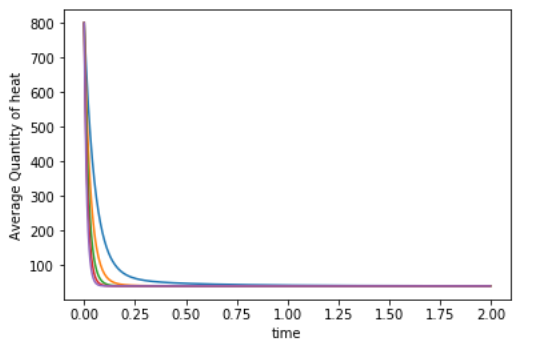
\includegraphics[width= \textwidth]{images/Barabasi-highest-degree.png}
     		\caption{}
     		\label{}
     	\end{subfigure}~
     	\begin{subfigure}[b]{0.45\textwidth}
     		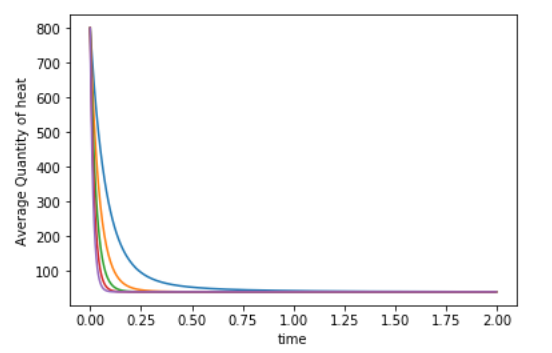
\includegraphics[width= \textwidth]{images/E-R-largest.png}
     		\caption{}
     		\label{}
     	\end{subfigure}\\
     	\begin{subfigure}[b]{0.45\textwidth}
     		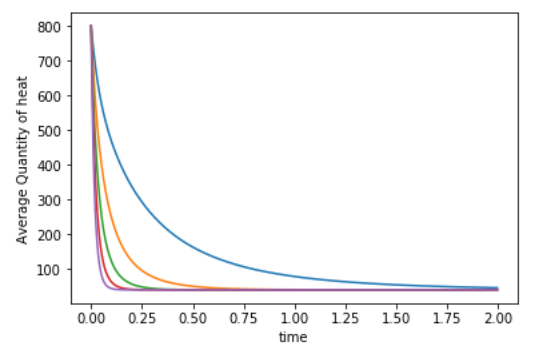
\includegraphics[width= \textwidth]{images/barabasi-random-selection.png}
     		\caption{}
     		\label{}
     	\end{subfigure}~
     	\begin{subfigure}[b]{0.45\textwidth}
     		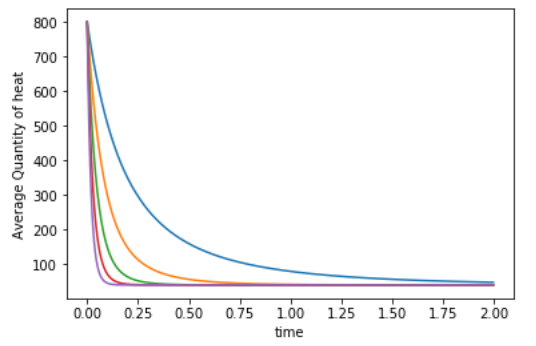
\includegraphics[width= \textwidth]{images/E-R-random.png}
     		\caption{}
     		\label{}
     	\end{subfigure}
     	\caption{ Results of the simulations for two networks. One is the Barabasi-Albert(BA) network and  the other is Erdos-Renyi(ER) network, both of $100$ nodes and average degree of $6$. Taking $5$ of the most important (by degree) nodes in the network from which diffusion is initiated by assigning certain quantities of heat to those nodes, the simulation of the diffusion is illustrated in plots (a) and (b) for the BA and ER networks respectively.}
     	\label{key}
     \end{figure}
     
     We observe that in BA network, heat spreads quite faster than in ER network that is to say by $t=0.6$, all the $5$ hubs in BA have levelled to equal amount while for ER, nodes still have un equal amounts of heat. This is because we assign quantities of heat to $5$ hubs of a network and they quickly spread heat to other nodes compared to ER where there are relatively fewer hubs among the five chosen nodes to initiate the diffusion process.
     
     \newpage
     
        \subsection{Diffusion on Directed Networks}
        A directed graph, also known as a Digraph or directed network, is one in which all the edges are directed from one vertex to another. 
        
        There are various complex systems whose skeleton can be captured by directed networks. Examples include ecological  networks, power grids, transportation networks, communication networks, metabolic networks, gene regulatory networks, citation networks among others. It is therefore paramount to study how dynamic processes such as diffusion, consensus, occur on such networks. There are various categories of directed networks which include:
        \begin{defn}[Weakly connected Digraph]
        	A directed graph is called weakly connected if replacing all of its directed edges with undirected edges produces a connected (undirected) graph.
          \end{defn}   
        \begin{defn}[Strongly connected Digraph]
        	A digraph is called strongly connected if and only if any two distinct nodes of the graph can be connected via a path that respects the orientation of the edges of the digraph \citep{saber2003agreement}.
        \end{defn}        
        For a strongly connected digraph with atleast two distinct nodes and with no self loops, the diffusion process on this network can be modelled in a similar manner as its undirected counterpart by 
        \begin{equation}
        \frac{d\boldsymbol{\phi}}{dt} = -C\mathbf{L}\boldsymbol{\phi}, \quad \boldsymbol{\phi}(0) = \boldsymbol{\phi}_0.
        \end{equation}
        For undirected graph $G$, the graph Laplacian,$L$, is symmetric positive semi-definite. However, for directed graphs $L$ is non-symmetric which implies that the diffusion on the former and latter graphs is not necessarily the same.
        
         \begin{defn}[Balanced Graphs]
        	We say the node $v_i$ of a digraph $G=(V,E)$ is balanced if and only if its in-degree and out-degree are equal, that is, $d_{out}(v_i) =d_{in}(v_i)$. A graph $G$ is balanced if and only if all its nodes are balanced, i.e $\sum_j a_{ij} = \sum_j a_{ji}, \forall i$. 
        \end{defn}
        
        \subsection{Diffusion and Equilibrium behaviour in Directed Network}
        In order to understand the process of attainment of steady state in networks, we need to study the spectral properties of graph Laplacian. Let $G=(V,E)$ be a digraph with Laplacian $L(G)$ with eigenvalues $\lambda_1, \lambda_2, \cdots, \lambda_n$ in non-decreasing order. 
        \subsubsection{Estimation of Eigenvalues of the Laplacian}
        Let $d_{max}$ be the maximum node out-degree of $G$, then following from Gershgorin disk theorem, then all the eigenvalues of $L(G)$ are located in the following disk
        \begin{equation} 
        D(G) = \{ z \in \mathbb{C} : |z-d_{max}| \leq d_{max} \}
        \end{equation}
        with centre at $z = d_{max} +0j$ in the complex plane \citep{saber2003agreement}. Thus, for a strongly connected digraph $G$, $L$ has a zero eigenvalue $\lambda_1=0$ and all the other non-trivial eigenvalues have non-negative real parts.
        Let us consider a strongly connected digraph $G=(V,E)$. Let $\boldsymbol{\phi}_0$ be the vector of quantities of heat at all nodes at $t=0$, $C=1$ be the diffusion coefficient. Similar to undirected case,the quantities of heat, $\boldsymbol{\phi}(t)$ at each node at a given time $t$ is given by
        \begin{equation}
        \boldsymbol{\phi}(t) = \boldsymbol{\phi}_0~e^{-\mathbf{L}t}.
        \end{equation}
        
        \begin{thm}[Limit Theorem for Exponential Matrices]
        	Assume $G$ is a strongly connected digraph with Laplacian $\mathbf{L}$ satisfying $\mathbf{L} \mathbf{v_r} = \mathbf{0}$, $\mathbf{v_{l} ^T} \mathbf{L} =\mathbf{0}$, and $\mathbf{v_{l} ^T} \mathbf{v_r}=1$. Then 
        	
        	\begin{equation}
        	 R = \lim_{t \longrightarrow +\infty} exp(-Lt) = v_r  v_{l} ^T \in M_n,
        	\end{equation}
        	where $M_n$ denotes a set of square $n\times n$ matrices, $v_r$,and $v_{l} ^T$ denote the right and left eigenvalues of $L$ associated with eigenvalue $\lambda_1 = 0$ \citep{saber2003agreement}.
        	\label{exponentialTheorem}
        \end{thm}
    From the theorem, we deduce that for a strongly connected digraph, equilibrium state can be attained and the quantity of heat at the nodes is given by
    \begin{equation}
    \lim_{t \longrightarrow \infty} =  \boldsymbol{\phi}_0  \mathbf{v_r}  \mathbf{v_{l} ^T}
    \label{equildirected}
    \end{equation}
    It is important to note that following Equation \ref{equildirected}, any equilibrium value $x^*$ can be attained such that $x^*_i =x^*_j$ for all $i$, $j$. This therefore motivates the search for which classes of digraphs attain equilibrium similar to that of undirected graphs where the value at each node is the average of the initial values at all nodes in the network.
    
    \begin{prop}
    Consider a directed network $G=(V,E)$ that is strongly connected. Then the digraph $G$ globally attains average equilibrium if and only if $\mathbf{1}^T \mathbf{L}= 0$.
    \label{prop1}
    \end{prop} 

    \subsubsection{Equilibrium state for Balanced Graphs}
     The proposition in \citep{saber2003agreement} states that 
     \begin{prop}
     Let $G=(V,E)$ be a digraph with an adjacency matrix $A=[a_{ij}]$ satisfying $a_{ii}=0, \forall i$. Then, all the following statements are equivalent:
     \begin{enumerate}[i)]
     	\item $G$ is balanced,
     	\item $\mathbf{v_l}= \mathbf{1}$ is the left eigenvector of the Laplacian of $G$ associated with the zero eigenvalue, that is, $\mathbf{1}^T \mathbf{L} = 0$.
     	\item $\sum_{i=1} ^ n u_i = 0, \forall x \in  \mathbb{R}^n$ with $u_i = \sum_{j \in N_i} a_{i,j} (x_j -x_i).$
     \end{enumerate}
     \label{prop1}
     \end{prop}
 
      Since for a balanced digraph $\mathbf{v_l}$ is an all ones vector, it therefore follows from Proposition \ref{prop1} that at equilibrium, the value at all nodes in a balanced graph is the average of the initial values at all nodes.
      
      \begin{exa}
      	Let us consider two directed graphs, one is a balanced digraph and the other is not. We then assign initial quantities of heat to all nodes in the order $0$ to $4$ as in the vector $\phi_0=[2,0,3,0,0]$ and set the diffusion coefficient, $C=1$. We then obtain plots for diffusion on both graphs after a specific time $t$ as shown in 
      	
      	\begin{figure}[H]
      		\centering
      	    \begin{subfigure}[b]{0.40\textwidth}
      	    	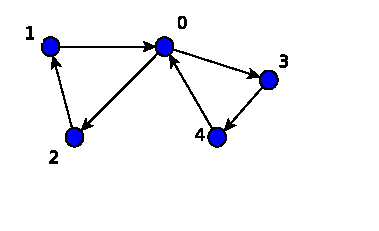
\includegraphics[width=\textwidth]{images/balanceDigraph.pdf}
      	    	\caption{}
      	    	\label{balanced-graph}
      	    \end{subfigure}~
      	    \begin{subfigure}[b]{0.5\textwidth}
      	    	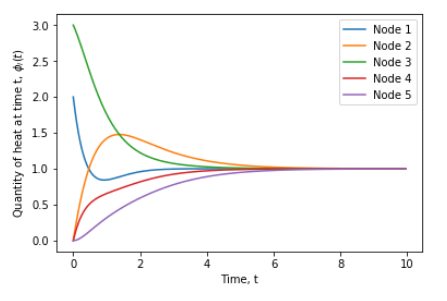
\includegraphics[width= \textwidth]{images/Balanced-digraph-diffusion.png}
      	    	\caption{}
      	    	\label{plot-balanced}
      	    \end{subfigure} \\
            \begin{subfigure}[b]{0.40\textwidth}
            	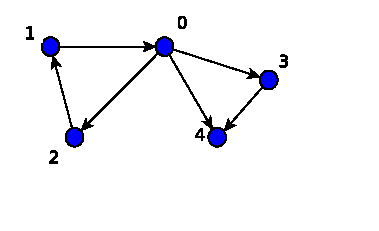
\includegraphics[width=\textwidth]{images/UnbalanceDigraph.pdf}
            	\caption{}
            	\label{unbalanced-graph}
            \end{subfigure}~
            \begin{subfigure}[b]{0.5\textwidth}
            	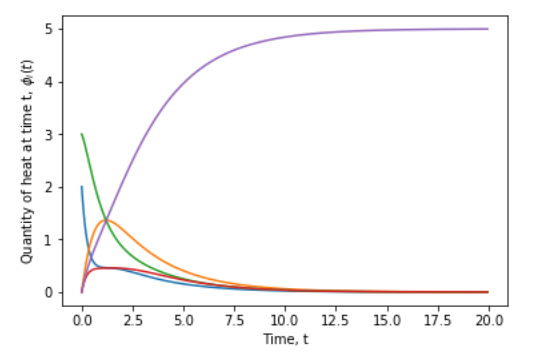
\includegraphics[width= \textwidth]{images/non-balnceddigraph-difusion.png}
            	\caption{}
            	\label{plot-unbalanced}
            \end{subfigure}
      		\caption{Diffusion over different categories of directed networks. (\subref{unbalanced-graph}) is an illustration of diffusion over weakly connected and unbalanced digraph in (\subref{balanced-graph}). (\subref{unbalanced-graph}) is an illustration of diffusion over strongly connected and balanced digraph (\subref{unbalanced-graph}).  }  
      		\label{unbalanced-diffusion}		
      	\end{figure} 
   For the balanced graph in Fig.~\ref{balanced-graph}, its Laplacian matrix $\mathbf{L}$,$v_r$ and $v_l$ are respectively:
   \begin{equation*}
   \mathbf{L} = \begin{pmatrix}
    2 &  0 & -1 & -1 &  0 \\
   -1 & 1  & 0  & 0  &  0 \\ 
    0 & -1 & 1  & 0  &  0 \\
    0 &  0 & 0  & 1  & -1 \\
    -1&  0 & 0  & 0  & 1
   \end{pmatrix}, \quad 
   v_r = v_l = \begin{pmatrix}
   0.4472136 \\  
   0.4472136 \\  
   0.4472136 \\ 
   0.4472136 \\
   0.4472136
   \end{pmatrix}
   \end{equation*} 
   The values for $v_r$ and $v_l$ satisfy Theorem \ref{exponentialTheorem} as well as Proposition \ref{prop1} and thus, equilibrium is attained at $x^*=1.0$ which is the average of initial values $x_0$.\\
   On the other hand, for the unbalanced graph in Fig.~\ref{unbalanced-graph}, we have the following matrices
    \begin{equation*}
   \mathbf{L} = \begin{pmatrix}
    3 &  0 & -1 & -1 & -1 \\
   -1 &  1 & 0  & 0  & 0  \\
    0 & -1 & 1  & 0  & 0  \\
    0 &  0 & 0  & 1  & -1 \\
    0 &  0 & 0  & 0  & 0
   \end{pmatrix}, \quad 
   v_r = \begin{pmatrix}
   0.4472136 \\  
   0.4472136 \\  
   0.4472136 \\ 
   0.4472136 \\
   0.4472136
   \end{pmatrix}, \text{ and }
   v_l = \begin{pmatrix}
   0.0 \\  
   0.0 \\  
   0.0 \\ 
   0.0 \\
   1.0
   \end{pmatrix}
   \end{equation*}
   We observe that $Lv_r = 0$ and $v_l^TL = 0$. However, the condition $v_l^T v_r = 1$  is not satisfied and therefore equilibrium cannot be attained as shown in Fig.~\ref{unbalanced-diffusion}. In addition, we observe that considering the structure, vertex $4$ has only in coming edges which signifies that during the diffusion process, vertex $4$ only receives heat from the immediate neighbours vertices $0$ and $3$ without giving out any due to lack of out going links. As a result, quantity of heat at vertex $4$ keeps on increasing as shown in Fig.~\ref{unbalanced-diffusion}.
   \end{exa}	
    \section{The Generalised Laplacian Matrix}
    	    
%    	    However, long-range interactions over networks have been evident in real world situations, for instance in attaining consensus in networked multi-agent systems, an agent is influenced not only by the nearest neighbours but also by the non-nearest neighbours. 
    	    
    	    
    	  
    	    There exists various ways in which the generalised matrix $L_G$ can be defined. In this work, however, we explore the elegant definition that is based on the $k$-path Laplacian matrices as introduced by Estrada in \citep{estrada2012path}. First, let us understand what the $k$-path Laplacian matrices are.
    	    \subsubsection{ k-path Laplacian matrices, $\mathbf{L}_k$}
    	    The k-path laplacian matrices are a natural generalisation of the combinatorial laplacian of a graph \citep{estrada2012path}. The motivation behind this generalisation is the idea of determining whether every node in a graph can be visited by means of a process that involves hopping from one node to another separated at a distance $k$. We can better understand the concept of k-path Laplacian through considering a polarisation process on a network, that is to say as, suppose a particle with a positive charge resides at a given node of simple graph $G= (V,E)$ and while at that node, it polarises all nodes at a distance $d$ from it. Consequently, the particle's movement to another is such that it hops to any nearest non-positively charged node. While at the new node, the particle polarises neighbouring nodes in the same manner as before. As a result, the particle either hops to the nearest non-positive nodes or returns to the origin node as illustrated in Fig. \ref{1-path-particle} and Fig.\ref{2-path-particle} for $d=1$ and $d=2$ respectively.
    	    
    	    
    	    \begin{figure}[!h]
    	    	\centering
    	    	\begin{subfigure}[b]{0.3\textwidth}
    	    		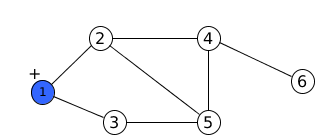
\includegraphics[width=\textwidth]{images/nodecharge1.png}
    	    		\caption{}
    	    		\label{particle1}
    	    	\end{subfigure}~
    	    	\begin{subfigure}[b]{0.3\textwidth}
    	    		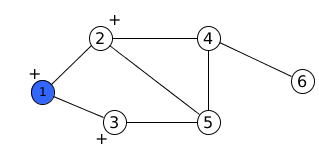
\includegraphics[width=\textwidth]{images/nodecharge11.png}
    	    		\caption{}
    	    		\label{polarity2}
    	    	\end{subfigure}~ 
    	    	\begin{subfigure}[b]{0.3\textwidth}
    	    		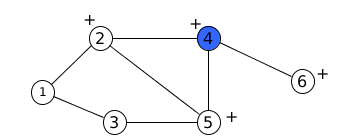
\includegraphics[width=\textwidth]{images/nodecharge2.png}
    	    		\caption{}
    	    		\label{polarity3}
    	    	\end{subfigure}
    	    	\caption{ Illustration of how the polarisation analogy used as a motivation for the $k$-path Laplacian concept for networks. Starting with a positively charged particle at node $1$ as shown in (\subref{polarity1}), taking $d=1$, the particle polarises all its nearest neighbours at a distance $d$ from it (that is nodes $2$ and $3$) as depicted in (\subref{polarity2}). The particle can therefore jump to the non-polarised nearest neighbours namely nodes $4$ and $5$ and $6$( though node $6$ is further compared to other two alternatives). Suppose the particle jumps to node $4$, similar polarisation process as the particle polarises the new nearest neighbours. The particle either jumps to node $3$ or returns to node $1$ as shown in (\subref{polarity3}).}
    	    	\label{1-path-particle}
    	    \end{figure}
    	    \vspace{1cm}
    	    
    	    \begin{figure}[H]
    	    	\centering
    	    	\begin{subfigure}[b]{0.3\textwidth}
    	    		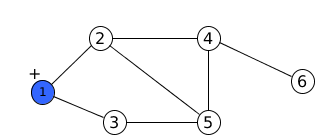
\includegraphics[width=\textwidth]{images/nodecharge1.png}
    	    		\caption{}
    	    		\label{polarityl21}
    	    	\end{subfigure}~
    	    	\begin{subfigure}[b]{0.3\textwidth}
    	    		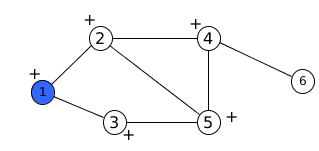
\includegraphics[width=\textwidth]{images/nodecharge41.png}
    	    		\caption{}
    	    		\label{polarityl22}
    	    	\end{subfigure}~ 
    	    	\begin{subfigure}[b]{0.3\textwidth}
    	    		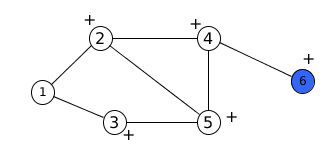
\includegraphics[width=\textwidth]{images/nodecharge4.png}
    	    		\caption{}
    	    		\label{polarityl23}
    	    	\end{subfigure}
    	    	\caption{Illustration of how the a charged particle navigates the network taking jumps of length $d=2$. As discussed before, a particle starting off at node $1$ will polarise neighbouring nodes separated at not more than distance $2$ from it (that is nodes $2$,$3$, $5$, and $4$) as shown in (\subref{polarityl22}). The particle then has only an option of jumping to the non-polarised node $6$ after which a similar process occurs again as in (\subref{polarityl23}). } \label{2-path-particle}
    	    \end{figure}
    	    
    	    As for the 'classical' case in which traversing the graph involves subsequent hops of length $1$ at a time, terminolgy such as walk, path, and many more are defined. In the same way, for the generalised case in which hops of various length not exceeding the diameter of a graph are taken into account,  we need to define terminology as well:\\
    	    \begin{defn}[k-hopping walk]
    	    	A k-hopping walk of length $l$ is any sequence of (not necessarily different) nodes $v_1,v_2, \cdots,v_l, v_{l+1}$ such that $d_{i,i+1} = k$ for each $i=1,2, \cdots, l.$ In otherwords, this walk is referred to as a k-hopping walk from $v_1$ to $v_{l+1}$ \citep{estrada2012path}.\\ 
    	    \end{defn}
    	    
    	    
    	    \begin{defn}[$k$-path degree]
    	    	The $k$-path degree $\delta_k(v_i)(k\leq d_{max})$ of a node $v_i$ is the number of irreducible shortest-paths of length $k$ having $v_i$as an endpoint \citep{estrada2012path}. \\
    	    \end{defn}
    	    \begin{defn}[$k$-path Laplacian matrix]
    	    	The $k$-path Laplacian matrix $L_k(k \leq d_{max})$ of a connected undirected graph $G=(V,E)$ is defined as the square symmetric $n \times n$ matrix whose entries are given by:
    	    	\begin{eqnarray}
    	    	L_k(ij) = \begin{cases} -1 &\mbox{if } d_{i,j} = k, \\
    	    	\delta_k(i) &\mbox{if } i = j,  \\
    	    	0 & \text{otherwise},
    	    	\end{cases}
    	    	\end{eqnarray}\label{k-laplacian}
    	    	where $d_{i,j}$ is the shortest path distance between nodes $i$ and $j$, $delta_{k}(i)$ known as the $k$-path degree is the number of irreducible shortest paths of length $k$ having node $i$ as an endpoint.\\
    	    \end{defn}
    	    
    	    \begin{exa}
    	    	Let us compute the $k$-path Laplacians for a simple graph $G$ in Fig.\ref{spanning}.
    	    	
    	    	\begin{figure}[H]
    	    		\centering
    	    		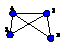
\includegraphics[width=0.25\textwidth]{images/compute-spanning.pdf}
    	    		\captionof{figure}{ A Graph of size 4.}
    	    		\label{spanning}
    	    	\end{figure}
    	    	
    	    	\begin{eqnarray*}
    	    		\mathbf{L_1(G)} = \begin{pmatrix}
    	    			2 & -1 & 0 & -1 \\
    	    			-1 & 3 & -1 & -1 \\
    	    			0 & -1 & 2 & -1  \\
    	    			-1 & -1 & -1 & 3
    	    		\end{pmatrix}, \quad
    	    		\mathbf{L_2(G)} = \begin{pmatrix}
    	    			1 & 0 & -1 & 0 \\
    	    			0 & 0 & 0 & 0 \\
    	    			-1 & 0 & 1 & 0 \\
    	    			0 & 0 & 0 & 0
    	    		\end{pmatrix}, \quad
    	    		\mathbf{L_3(G)} = \begin{pmatrix}
    	    			0 & 0 & 0 & 0 \\
    	    			0 & 0 & 0 & 0 \\
    	    			0 & 0 & 0 & 0 \\
    	    			0 & 0 & 0 & 0
    	    		\end{pmatrix}
    	    	\end{eqnarray*}\\
    	    \end{exa}
    	    
%    	    The $k$-path Laplacian matrix $\mathbf{L}_{k} (k \leq d_{max})$ of a connected undirected graph $G=(V,E)$ is defined as the square symmetric $n\times n$ matrix whose entries are given by:
%    	    \begin{equation}
%    	    \mathbf{L}_k(i,j) =  \begin{cases*}
%    	    -1 & if  $d_{i,j} = k,$  \\
%    	    \delta_{k}(i) & if $i = j,$ \\
%    	    0 & otherwise.
%    	    \end{cases*}
%    	    \label{kpathlap}
%    	    \end{equation}
    	    
    	    
    	    
    	    The concept of $k$-path Laplacians defined in Eqn \ref{k-laplacian} for finite undirected graphs was extended for connected and locally finite infinite graphs as follows:
    	    Consider $\Gamma = (V,E)$ to be an indirected finite or infinite graph with vertices $V$ and edges $E$. We assume that $\Gamma$ is connected and locally finite that is to say each vertex has only finitely many edges emanating from it. Let $d$ be the distance metric on $\Gamma$, i.e. $d(v,w)$ is the length of the shortest path from $v$ to $w$, and let $\delta_{k}(v)$ be the $k$-path degree of the vertex $v$, i.e.
    	    \begin{equation}
    	    \delta_{k}(v) := \#\{w \in V : d(v,w) = k\}.
    	    \end{equation}
    	    Since $\gamma$ is locally finite, $\delta_{k}(v)$ is finite for every $v \in V$. Denote by $C(V)$ the set of all complex-valued functions on $V$ and by $C_{0}(V)$ the set of the complex-valued functions on $V$ with finite support. Moreover, let $\ell^2(V)$ be the Hilbert space of square-summable functions on $V$ with inner product
    	    \begin{equation}
    	    \langle f,g\rangle = \sum_{v\in V} f(v) \overline{g(v)}, \quad f,g \in \ell^2(V) 
    	    \end{equation}
    	    In $\ell^2(V)$ there is a standard orthonormal basis consisting of the vectors $e_v, v\in V$, where
    	    \begin{equation}
    	    e_v(w) :=  \begin{cases*}
    	    1 & if  w = v,  \\
    	    0 & otherwise.
    	    \end{cases*}
    	    \end{equation}
    	    Let $\mathbf{L}_{k}$ be the following mapping from $C(V)$ into itself:
    	    \begin{equation}
    	    (\mathbf{L}_{k}) (f) := \sum_{w\in V: d(v,w)=k} (f(v) -f(w)), \quad f \in C(V).
    	    \label{infinite-dif}
    	    \end{equation}
    	    
    	    
    	    \begin{defn}[k-hopping connected component]
    	    	A $k$-hopping connected component in a graph $G=(V,E)$ is a subgraph $G' = (V',E')$, $V'\subset V,E' \subset E$, such that there is at least one $k$-hopping walk that visit every node $v_i \in V'$.
    	    	As mentioned earlier, the motivation of the generalisation of graph Laplacian to find the solution of the problem of whether a given graph can be $k$-hopped. If not, how many $k$-hopping connected components exist?\\
    	    \end{defn}
    	    \begin{thm}
    	    	The number of $k$-hopping connected components in a connected undirected graph $G=(V,E)$ is given by $\eta_k(G) = m[\lambda_1(L_k)=0]$ \citep{estrada2012path}.\\
    	    \end{thm}
        
    	    \begin{proof}
    	    	Let us consider a simple undirected graph $G$ that is connected, in otherwords a graph that can be $1$-hopped. Let ${v_1, v_2, \cdots, v_n}$ be an orthogonal basis of $\mathbb{R}^n$ such that $\mathbf{L} \mathbf{y}_j = \lambda_j (\mathbf{L}) \mathbf{y}_j$. Using Rayleigh-Ritz Principle we obtain
    	    	\begin{equation}
    	    	\lambda_1(\mathbf{L}) = \min\limits_{\mathbf{y} \in \mathbb{R}^n \ \{\mathbf{0} \}} \frac{\mathbf{y}^T \mathbf{L} \mathbf{y}}{\mathbf{y}^T \mathbf{y}} =
    	    	\min\limits_{\mathbf{y} \in \mathbb{R}^n \ \{\mathbf{0} \}}
    	    	\frac{\sum_{p,q \in P(v_p,v_q)} (y_p -y_q)^2}{\sum_{p\in V} y_p ^2}
    	    	\end{equation}
    	    	Let $\mathbf{y}$ be an eigenvector of $\mathbf{L}$ with eigenvalue $\lambda_i(\mathbf{L}_k)=0$. This implies that
    	    	\begin{equation}
    	    	\mathbf{y}^T \mathbf{L} \mathbf{y} = \frac{1}{2} \sum_{p,q \in P(v_p,v_q)} (y_p-y_q)^2 , 
    	    	\label{equatezero} 
    	    	\end{equation}
    	    	Equation \ref{equatezero} holds if $y_p = y_q$ which happens if and only if the two vertices $v_p$ and $v_q$ are connected which implies that for all vertices connected by a path in the network, $\mathbf{y}$ should be a constant.
    	    	which happens if and only if, $y_p =y_q$ for each pair of nodes which are connected by an edge. However, on assumption that $G$ is connected, it implies that each pair of vertices of the connected component can be connected by a path and thus $y_p =y_q$ for all pair of vertices of the connected component. Consequently, for a one connected component, the vector $\mathbf{v}= \mathbf{0}$ is the only vector with corresponding to eigenvalue of $0$. In otherwise, $\mathbf{v}$ is a constant vector spanning a dimensional space. 
    	    	
    	    	Let us now consider the case of $n$ connected components. Suppose graph $G$ is made of vertices arranged, without loss of generality, in way that its Laplacian matrix is organised as 
    	    	\begin{equation*}
    	    	\mathbf{L} = \begin{pmatrix}
    	    	L_{1} & 0 & \cdots & 0 \\
    	    	0 & L_{2} & \cdots & 0\\
    	    	\vdots& \vdots & \ddots & \vdots \\
    	    	0 & 0 & \cdots & L_{n}
    	    	\end{pmatrix}.
    	    	\end{equation*}
    	    	The spectrum of the block diagonal matrix $\mathbf{L}$ is given as the union of the spectra of blocks $\mathbf{L_i}$. The corresponding eigenvectors are given as those of $\mathbf{L_i}$ with zeroes at the positions of other blocks.
    	    	Since $\mathbf{L_i}$ is a graph laplacian for a connected component and we know that each $\mathbf{L_i}$ has $0$ as an eigenvalue with multiplicity $1$, it therefore implies that the multiplicity of $0$ as an eigenvalue of $L$ corresponds to the number of connected components in the graph $G$ \citep{von2007tutorial}. 
    	    	
    	    	Let us now consider a graph that can be $k$-hopped that is to say graph with only $1$ k-connected component for $k>1$. The graph Laplacian $\mathbf{L_k}$ is defined as in Equation \ref{k-laplacian}. Following similar argument as the case of $1$-hopped graph discussed before, we have
    	    	\begin{equation}
    	    	\mathbf{y}^T \mathbf{L_k} \mathbf{y} = \sum_{p,q \in P_k(v_p,v_q)} (y_p-y_q)^2 = 0,  
    	    	\end{equation} 		
    	    	which happens if and only if, $y_p =y_q$ for each pair of nodes which are connected by the shortest-path of length $k$. Now, let us assume that the graph is k-hopping connected. Then, because every pair of nodes is connected by paths of length $ck$, we have that $y_p =y_q \neq 0$ for every pair of nodes in the graph. Consequently, $\mathbf{y}$ is a constant vector spanning a one-dimensional space.
    	    	
    	    	Now let $j>1$ and let us assume that the graph has $g$ $k$-hopping connected components $\mathbf{L_{k}^1,L_{k}^2,\cdots, L_{k}^g }$. Then, the $k$-Laplacian matrix can be written as:
    	    	\begin{equation*}
    	    	\mathbf{L}_k = \begin{pmatrix}
    	    	L_{k}^1 & 0 & \cdots & 0 \\
    	    	0 & L_{k}^2 & \cdots & 0\\
    	    	\vdots& \vdots & \ddots & \vdots \\
    	    	0 & 0 & \cdots & L_{k}^g
    	    	\end{pmatrix}.
    	    	\end{equation*}
    	    	Following similar arguments as for the case of the $k$-hopping connected graph it can be seen that $\mathbf{L}_k$ has $g$ orthogonal eigenvectors $\mathbf{y}_j$ of eigenvalue $0$, such that $y_p = y_q \neq 0$ for each pair of nodes which are in the same $k$-connected of the graph and zero otherwise \citep{estrada2012path}.\\  	
    	    \end{proof}
    	    
    	    \begin{exa}
    	    	Let us consider the graph, G in Fig.~\ref{spanning}, since $d_{max} = 2$ we compute the 1-hopping and 2-hopping connected components of G.
    	    	
    	    	\begin{table}[H]
    	    		\centering
    	    		\begin{tabular}{ |l|l|c|l| }
    	    			\hline
    	    			& & no. of components & components \\
    	    			\hline
    	    			\multirow{4}{*}{$\lambda_i(\mathbf{L}_1)$} & $\mathbf{0.000}$& & \\
    	    			& 2.000& 1& 1- 2- 3- 4\\
    	    			& 4.000 & & \\
    	    			& 4.000 & & \\ \hline
    	    			\multirow{4}{*}{$\lambda_i(\mathbf{L}_2)$} & $\mathbf{0.000}$& & \\
    	    			& $\mathbf{0.000}$& 3 & 1-3,\\
    	    			& $\mathbf{0.000}$ &  & 2,\\
    	    			& 2.000 &  & 4\\
    	    			\hline
    	    		\end{tabular}   
    	    	\end{table}
    	    	
    	    	
    	    \end{exa}
    	    
    	    \subsection{k-path Laplacian for Weighted Networks}
    	    For a weighted network, The weight of a path between two nodes $u$ and $v$ separated by $k$ edges, is the sum of the weights along the path. The entries of $k$-path Laplacian matrices are, therefore, given by
    	    
    	    \begin{equation}
    	    \mathbf{L}_k(i,j) = \begin{cases} -d_{i,j} &\mbox{if } e_p(ij) = k, \\
    	    \sum_{j} d_{ij} &\mbox{if } i = j , \\
    	    0 & \text{otherwise}.
    	    \end{cases}
    	    \end{equation}
    	    where $e_p(ij)$ is the number of edges long the shortest path between nodes $p$ and $q$.\\
    	    
    	    \begin{exa}
    	    	Let us consider aa simple weighted graph in Fig.~\ref{weighted}.
    	    	\begin{figure}[!h]
    	    		\centering
    	    		\vspace{0pt}
    	    		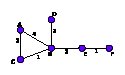
\includegraphics[width= 0.35\textwidth]{images/centralities-weighted.pdf}
    	    		\caption{ A weighted network with $6$ nodes and $6$ weighted edges.} \label{weighted}
    	    	\end{figure} 
    	    	
    	    	\begin{table}[!h]
    	    		\centering
    	    		\begin{tabular}{ |l|l|c|l| }
    	    			\hline
    	    			& & no.of components(computed) & no. of components (actual)\\
    	    			\hline
    	    			\multirow{6}{*}{$\lambda_i(\mathbf{L}_1)$} 
    	    			& 12.3472& & \\
    	    			& 5.7468 & & \\
    	    			& $\mathbf{0.0000}$ & & \\
    	    			& 0.7503 & 1&1 i.e  \\
    	    			& 2.0000 & & A-C-B-D-B-E-F\\
    	    			& 3.1558 & & \\
    	    			\hline
    	    			\multirow{6}{*}{$\lambda_i(\mathbf{L}_2)$} 
    	    			& 19.6847& &\\
    	    			& 7.3153 & & \\
    	    			& $\mathbf{0.0000}$ &2 & 2 i.e\\
    	    			& $\mathbf{0.0000}$ & &A-E-C-D, B-F \\
    	    			& 6.0000 & & \\
    	    			& 17.000 & & \\
    	    			\hline
    	    			\multirow{6}{*}{$\lambda_i(\mathbf{L}_3)$} 
    	    			& 21.7251& &\\
    	    			& $\mathbf{0.0000}$ & & \\
    	    			& 5.9228 &3 & 4 i.e\\
    	    			& 4.3521 & &A-F-C-F-D, E,B \\
    	    			& $\mathbf{0.0000}$ & & \\
    	    			& $\mathbf{0.0000}$ & & \\
    	    			\hline
    	    		\end{tabular}   
    	    		\caption{k-hopping components of a graph in Fig.\ref{weighted}} 
    	    		\label{tablecomponentsg1}
    	    	\end{table}
    	    	
    	    	From Table.~\ref{tablecomponentsg1}, we observe that for $k=1$ and $k=2$, the number of components computed based on the multiplicity of the smallest eigenvector corresponds with the number of components obtained through navigating the graph (actual value). However, for $k=3$, we observe inconsistency in the two values.\\
    	    \end{exa}
    	    
    	    \begin{exa}
    	    	Let us consider a simple weighted graph in Fig.~\ref{weighted}.
    	    	\begin{figure}[!h]
    	    		\centering
    	    		\vspace{0pt}
    	    		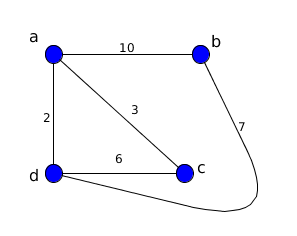
\includegraphics[width= 0.35\textwidth]{images/weighted2.png}
    	    		\caption{ A weighted network with $6$ nodes} \label{weighted3}
    	    	\end{figure} 
    	    	
    	    	\begin{table}[!h]
    	    		\centering
    	    		\begin{tabular}{ |l|l|c|l| }
    	    			\hline
    	    			& & no.of components(computed) & no. of components (actual)\\
    	    			\hline
    	    			\multirow{4}{*}{$\lambda_i(\mathbf{L}_1)$} 
    	    			& 26.1073 & & \\
    	    			& 0.0000 & 1 &1 \\
    	    			& 8.8606 & & \\
    	    			& 14.0321& & \\
    	    			\hline  
    	    			\multirow{4}{*}{$\lambda_i(\mathbf{L}_2)$} 
    	    			& 26.0000& &\\
    	    			& $\mathbf{0.0000}$ &3 & 3 i.e\\
    	    			& $\mathbf{0.0000}$ & &b-c, a, d\\
    	    			& $\mathbf{0.0000}$ & & \\
    	    			\hline 
    	    		\end{tabular}   
    	    		\caption{k-hopping components of a graph in Fig.\ref{weighted}} 
    	    		\label{tablecomponentsg1}
    	    	\end{table}
    	    	The diameter of the graph is $2$. Computations for $k-$ hopping components for $k=1$ and $k=2$ correspond to the actual number as drawn from the graph.
    	    \end{exa}
    	    
    	    \begin{exa}
    	    	Let us consider a simple weighted graph in Fig.~\ref{weighted3}.
    	    	\begin{figure}[!h]
    	    		\centering
    	    		\vspace{0pt}
    	    		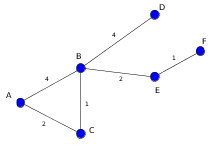
\includegraphics[width= 0.5\textwidth]{images/weighted3.png}
    	    		\caption{ A weighted network with $6$ nodes} \label{weighted3}
    	    	\end{figure} 
    	    	\begin{table}[H]
    	    		\centering
    	    		\begin{tabular}{ |l|l|c|l| }
    	    			\hline
    	    			& & no.of components(computed) & no. of components (actual)\\
    	    			\hline
    	    			\multirow{6}{*}{$\lambda_i(\mathbf{L}_1)$} 
    	    			& 14.7000& & \\
    	    			& 6.3200 & & \\
    	    			& $\mathbf{0.0000}$ & & \\
    	    			& 0.7600 & 1&1 \\
    	    			& 2.6800 & & \\
    	    			& 3.5500 & & \\
    	    			\hline
    	    			\multirow{6}{*}{$\lambda_i(\mathbf{L}_2)$} 
    	    			& $\mathbf{0.0000}$& &\\
    	    			& 9.4900 & & \\
    	    			& 25.9000 &2 & 2 i.e\\
    	    			& 20.6000 & &A-E-C-D, B-F \\
    	    			& $\mathbf{0.0000}$ & & \\
    	    			& 6.0000 & & \\
    	    			\hline
    	    			\multirow{6}{*}{$\lambda_i(\mathbf{L}_3)$} 
    	    			& 24.4100& &\\
    	    			& $\mathbf{0.0000}$ &3 & 3 i.e\\
    	    			& 7.0000 & &A-F-D-F-C, E,B \\
    	    			& $\mathbf{0.0000}$ & & \\
    	    			& $\mathbf{0.0000}$ & & \\
    	    			& 4.5900& &\\
    	    			\hline
    	    		\end{tabular}   
    	    		\caption{k-hopping components of a graph in Fig.\ref{weighted3}} 
    	    		\label{tablecomponentsg3}
    	    	\end{table}
    	    	
    	    	From Table.~\ref{tablecomponentsg3}, we observe that for $k=1$ and $k=2$, the number of components computed based on the multiplicity of the smallest eigenvector corresponds with the number of components obtained through navigating the graph (actual value). However, for $k=3$, we observe inconsistency in the two values.
    	    \end{exa}
    	    
    	    Following from the definition of the $k$-path Laplacian matrices, we thus define the generalised Laplacian matrix as
    	    \begin{equation}
    	    L_{G} = \sum_{k=1}^{\Delta} c_{k}L_{k}
    	    \end{equation}
			where $1 \leq \Delta \leq d_{max}$ and $c_k$ are the coefficients.
		    The coefficients $c_k$ play a crucial role in the generalisation of diffusion process on network and so determining the values of these coefficients is an important task. The values of $c_k$ are expected to give more weight to shorter than to the longer range interactions. In \citep{estrada2012path} Estrada proposed two approaches categorised as social and physical ways of influence.
		    
		    \subsection{Properties of the Generalised Laplacian Matrix }
		    The generalised matrix $L_G$ is real and symmetric. It is also a semi-positive definite matrix as shown in the proof:
		    \begin{proof}
		    	For any column vector $\mathbf{y}$
		    	\begin{equation}
		    	\mathbf{y}^T L_{G} \mathbf{y} = \mathbf{y}^T(c_{1}L_{1} + c_{2}L_{2} + \cdots + c_{\delta}L_{\delta} )\mathbf{y}
		    	= \mathbf{y}^Tc_{1}L_{1}\mathbf{y} + \mathbf{y}^Tc_{2}L_{2}\mathbf{y} + \cdots + \mathbf{y}^Tc_{\delta}L_{\delta}\mathbf{y} 
		    	\end{equation}
		    	Since $\mathbf{y}^Tc_{k}L_{k}\mathbf{y} \geq 0$ for $c_{k}>0$ and $1 \leq k \leq \delta$ as in Eqn.\ref{equatezero}, then
		    	\begin{equation}
		    	\mathbf{y}^T L_{G} \mathbf{y} \geq 0	
		    	\end{equation}
		    \end{proof}
		    %    	    	 \subsubsection{Spectrum of the Generalised Laplacian matrix}
		    The spectrum of the Laplacian matrix is the set of eigenvalues and their multiplicities \citep{estrada2011epidemic}. Let $\lambda_1 < \lambda_2 < \cdots < \lambda_n$ be the eigenvalues of $L(x)$ and their corresponding multiplicities $m(\lambda_1), m(\lambda_2), \cdots, m(\lambda_n)$. The spectrum of $L$ is given by
		    \begin{equation}
		    S_p L = \big(\lambda_1 \quad \lambda_2 \quad \cdots \quad \lambda_n \\
		    m(\lambda_1) \quad m(\lambda_2) \quad \cdots \quad m(\lambda_n)  \big).!h
		    \end{equation}
		    Some analytical expressions for the spectra of the Laplacian matrix of some common simple networks are:\\
		    \begin{itemize}
		    	\item Star, $S_n$: $S_p(L) = {0~ 1^{n-2}~ n}$\\
		    	\item Path, $P_n$: $S_p(L) = {2-2\cos\big( \frac{\pi(j-1)}{n}\big) }$
		    \end{itemize}
		    For generalised Laplacian matrix $L(x)$, the above expressions as a function of conductance $x$ are given by
		    \begin{itemize}
		    	\item Star, $S_n$: $S_p(L(x)) = {0~ (1+8x)^{n-2}~ n}$\\
		    	\item Path, $P_n$: $S_p(L(x)) = { }$
		    \end{itemize}
		    \begin{figure}[H]
		    	\centering
		    	\begin{subfigure}[b]{0.45\textwidth}
		    		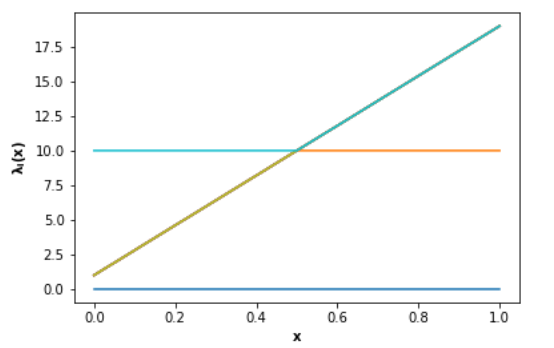
\includegraphics[width= \textwidth]{images/Star-network-eigenplot.png}
		    		%\caption{$x=0.1, t=0.5$}
		    		\label{star-spectra}
		    	\end{subfigure}~
		    	\begin{subfigure}[b]{0.45\textwidth}
		    		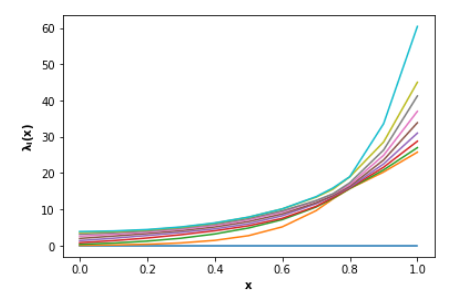
\includegraphics[width= \textwidth]{images/Path-network-eigenplot.png}
		    		%\caption{$x=0.1, t=3.0$}
		    		\label{path-spectra}
		    	\end{subfigure} \\
		    	\begin{subfigure}[b]{0.85\textwidth}
		    		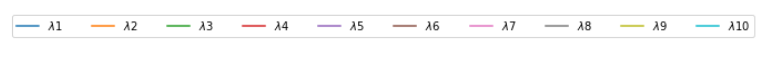
\includegraphics[width= \textwidth]{images/legend-eigenvalues.png}
		    		%\caption{$x=0.1, t=3.0$}
		    		%\label{gridt3x01}
		    	\end{subfigure}
		    	\caption{Illustrations of variation of eigenvalues with conductance $x$ two networks.
		    		(\subref{star-spectra}) corresponds to that a star network, $S_{10}$ and  (\subref{path-spectra}) corresponds to that of a path graph, $P_{10}$}.
		    	\label{eigen-xvalues}
		    \end{figure}
		    As discussed before, the eigenvalues $\lambda_i(x)$ of the Laplacian matrix $L(x)$ are an increasing function of $x$ except for the smallest eigenvalue $\lambda_1(x) = 0$ which remains almost constant as observed in Figure \ref{eigen-xvalues}. For the star network , both $\lambda_1(x) = 0$ and $\lambda_1(n) = 5$ remain constant the analytical expressions mentioned before. However, the rest of the eigenvalues increase linearly with increase in $x$ values. At $x=0.5$, we observe that all eigenvalues are equal with a value of $10$. This is because at $x=0.5$, all edges of the star network have a weight of $1$ and thus, a complete network,$K_n$, whose spectrum is given by $S_p(L) = \{0~ n^{n-1} \}$. On the other hand, the path network follows a similar trend as that of the star network but the $x$ value at which all eigenvalues (except $\lambda_i=0$) are equal is relatively higher than $0.5$ that is to say the point lies at $x=0.7$. 
    	    \subsubsection{Social Influence}    	
    	    	Here we consider a social network where nodes represent the people with in a society and the links are the social relationship or ties among the people for instance friendship, family relations, collaboration, among others. In such networks, influence between two people connected to each other in the network can be accounted for. However, it is quite challenging to account for the indirect influence between two people that are not directly connected in the network. An approach introduced in \citep{estrada2011epidemic}considers that which on empirical evidence, the indirect influence or long range interactions among people can be thought of as a pre-conditioner for establishment of a new social tie. In otherwords, new social ties among humans are created as an investment in the future as justified by empirical evidence in \citep{estrada2011epidemic}. it is quite obvious that two individuals that influence each other, probability is high that the two become friends compared to those that have no mutual influence. This process can be considered as an analogy in which the future value of money, in particular the future
    	    	value of a growing annuity, is determined in quantitative finance but for this case we consider a transaction involving information instead of money. Suppose an individual A lends information to individual B whose present value is $PVI$ at an interest rate $r$ and for a time period $t$. The future value of the information $FVI$ is given by
    	    	\begin{equation}
    	    	FVI = PVI (1+r)^t
    	    	\end{equation}
    	    	Let us consider the process on a network where node $v_1$ lends information to node $v_(l+1)$. On assumption that information flows through the shortest path and considering a discrete time at every step, the information is transfered from $v_1$ to nearest neighbour $v_2$ at a value $A$ and rate $r$. At $v_2$, the present value $PVI=A/(1+r)$. The information is enriched at $v_2$ at a growing rate of $g$ and then transferred to $v_3$. The process is repeated as before and at each node information is enriched before transfer to the next node. Finally, the information at borrower node $v_(l+1)$ is $A ( 1 + g )^ {l -1} /( 1 + r )^l$. Thus, The cumulative present
    	    	value of the information in this process is given by the sum of all the values at the nodes of the chain, that is,
    	    	\begin{equation}
    	    	PVI
    	    	= A /( 1 + r ) + A ( 1 + g )/( 1 + r )^2 + \cdots + A ( 1 + g )^(l -1) /( 1 + r )^l .
    	    	\end{equation}
    	    	Suppose $g=r$ and $A=1$ for the sake of simplicity, for a connected network with shortest distance between any pair of nodes denoted by $d_{i,j}$, the future value of information transmitted from $i$ to $j$ is:
    	    	
    	    	\begin{equation}
    	    	FVI_{i,j} = d_{i,j} x^{d{i,j}-1},
    	    	\end{equation}
    	    	where $x = 1+r = 1+g$.
    	    	Thus, from the analogy, we can consider that the mutual influence between two nodes separated at distance $k$ is given by the future value of the investment that the creation of a new link will represent to them. 
    	    	
    	    	For the social influence, we can define the coefficients in Eqn. \ref{kgen-difeqn} as $c_1 =1 $ and $c_{k \geq 2} = k x^{k-1}$
    	    	, where $0 < x < 1 / 2$. The empirical parameter $x$ also known as the conductance in \citep{estrada2011epidemic} controls the strength of interaction between nodes $i$ and $j$ separated at distance $k$. This implies that the strength of the casual contact  between two nodes reduces with increase in social distance between them.
    	    	
    	    	The generalised Laplacian matrix for which long-range interactions are accounted for by the social influence is given as 
    	    	\begin{eqnarray}
    	    	L_{G,x} = \begin{cases} \delta_{Gv_i} &\mbox{if } i = j \\
    	    	-1 &\mbox{if } i \neq j \text{ and } v_i \text{ is adjacent to } v_j \\
    	    	-k x^{k-1} & \text{otherwise},
    	    	\end{cases}
    	    	\end{eqnarray}
    	    	where $\delta_{Gv_i}$ denotes the generalised degree.
    	    	 In modelling the spread of epidermic, Estrada in \citep{estrada2011epidemic} considered two types of contacts that is   close contacts  which are frequent interactions among individuals and casual or long range interactions are the non frequent encounters among individuals which facilitate the spread of infections.The latter which were considered as non-random where accounted by use of the social influence approach.
    	    	 
    	    	 
    	    	
    	    	\subsection{Physical Influence}
    	    	It is observed in many man-made and naturally evolving systems that communication among the agents of the system follows a spatial decay as illustrated in sensor systems where sensors far away from the target display low noise-signal ratio as a result of attenuation (spatial decay) of signal energy, in earthquake incidences where the aftershocks follow a spatial decay, that is, areas further from the main shock are less affected compared to nearer areas. This spatial decay takes on the form $r ^{-\alpha}$ , where $r$ is the distance from the main shock. Other examples of similar physical scenarios include the brain in which the interconnectivity certain neurons in mammalian neo-
    	    	cortex decays exponentially with the intersomatic distance, and many others.
    	    	According to Estrada \citep{estrada2012path}, the spatial decay can take on two forms namely:
    	    	
    	        \begin{enumerate}[i)]
    	    	\item Exponential form
    	    	For the exponential form, Eqn.\ref{kgen-difeqn} attains a generalised form based on the Laplace-transformed $k$-Laplacian:
    	    	\begin{equation}
    	    	\tilde{\mathbf{L}}_{L,\lambda} = \mathbf{L} + \sum_{k=2}^{\infty} e^{-\lambda k} \mathbf{L}_k, 
    	    	\label{laplacetransform}
    	    	\end{equation}
    	    	where $\lambda >0$ is a parameter that depends on the specific situation to be modelled.
    	    	Thus, the coefficients of Eqn.\ref{kgen-difeqn} are $c_1 = 1$ and $c_{k \geq 2} = e^{-\lambda k}$.
    	    	
    	    	\begin{figure}[H]
    	    		\centering
    	    		\begin{subfigure}[b]{0.45\textwidth}
    	    			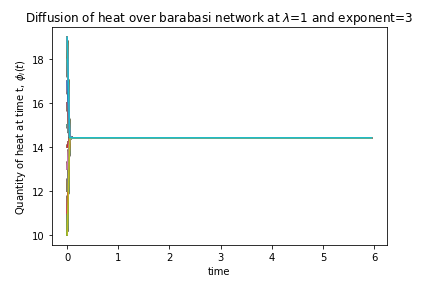
\includegraphics[width=\textwidth]{images/BA-lam1-laplace.png}
    	    			\caption{$\lambda=1$}
    	    			%\label{barabasi-x0}
    	    		\end{subfigure}~
    	    		\begin{subfigure}[b]{0.45\textwidth}
    	    			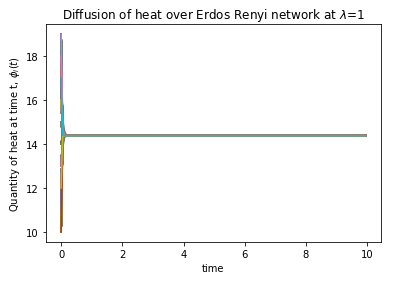
\includegraphics[width= \textwidth]{images/ER-lam1-laplace.png}
    	    			\caption{$\lambda=1$}
    	    			%\label{erdos-x01}
    	    		\end{subfigure}\\
    	    		\begin{subfigure}[b]{0.45\textwidth}
    	    			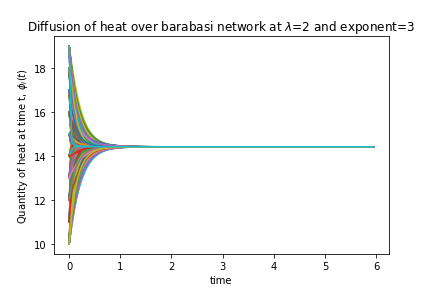
\includegraphics[width= \textwidth]{images/BA-lam2-laplace.png}
    	    			\caption{$\lambda=2$}
    	    			%\label{barabasi-x02}
    	    		\end{subfigure}~
    	    		\begin{subfigure}[b]{0.45\textwidth}
    	    			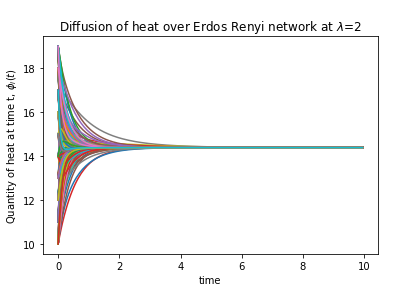
\includegraphics[width= \textwidth]{images/ER-lam2-laplace.png}
    	    			\caption{$\lambda=2$}
    	    			%\label{erdos-x02}
    	    		\end{subfigure}\\
    	    		\begin{subfigure}[b]{0.45\textwidth}
    	    			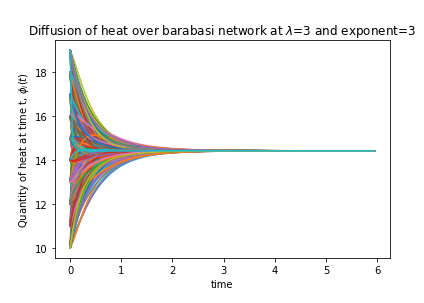
\includegraphics[width= \textwidth]{images/BA-lam3-laplace.png}
    	    			\caption{$\lambda=3$}
    	    			%\label{barabasi-x04}
    	    		\end{subfigure}~
    	    		\begin{subfigure}[b]{0.45\textwidth}
    	    			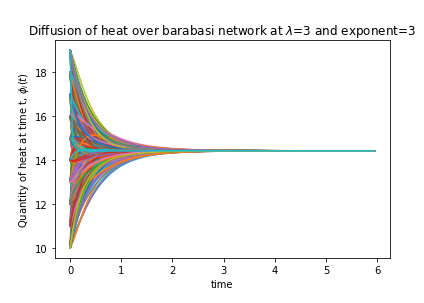
\includegraphics[width= \textwidth]{images/BA-lam3-laplace.png}
    	    			\caption{$\lambda=3$}
    	    			%\label{erdos-x04}
    	    		\end{subfigure}
%    	    		\caption{Barabasi networks (left) and Erdos Renyi networks(right) of 1000 nodes and average degree of 6. Top row is illustration of diffusion process at $x=0$ ( i.e accounting for direct interactions only), middle row corresponds to $x=0.2$ followed by $x=0.4$ in the last row}
%    	    		\label{barabasi-Erdos-compare}
    	    	\end{figure}
%    	    	\item The factorial-transformed $k$-Laplacian
%    	    	\begin{equation}
%    	    	\tilde{\mathbf{L}}_{F,z} =  \mathbf{L} + \sum_{k=2}^{\infty} \frac{z^k}{k!} \mathbf{L}_k 
%    	    	\end{equation}
				
    	    	\item Power-law 
    	    	Here, we use the Mellin transform of $k$-Laplacian matrices to obtain the generalised equation:
    	    	\begin{equation}
    	    	\tilde{\mathbf{L}}_{M,s} = \sum_{k=1}^{\infty} k^{-s} \mathbf{L}_k,
    	    	\label{mellin-transforms}
    	    	\end{equation}
    	    	where $\lambda >0$ is a parameter that depends on the specific situation to be modelled and the coeffients of Eqn.\ref{kgen-difeqn} are $c_{k} = k^{-s}$. 	
    	    	In \citep{estrada2017path}, it is shown that normal diffusion occurs only when $s > 3$. On the other hand, superdiffusion occurs when $1 <s < 3$ with superdiffusive exponent being $ \kappa = \frac{2}{s-1}$,
    	    	which leads to arbitrary values for $\kappa \in (1,\infty)$. 
    	    	The Mean Square Distance, $MSD \sim t^\kappa$. Normal diffusion is attained  at $\kappa =1$, superdiffusion is attained at $\kappa > 1$. However, a special type of diffusion known as Ballistic diffusion is characterised by the fact that at small times the particles are not hindered yet
    	    	by collisions and diffuse very fast. It is attained at $\kappa = 2$.
    	    \end{enumerate}
        \subsection{The Long Range Interaction Model LRI-model}
        We consider that given a simple graph $G=(V,E)$ with diameter denoted by $d_{max}$. Its $k$-path Laplacian matrices can be transformed in various ways. However, in this work we consider two types of transforms as covered in \citep{estrada2017path} namely the Mellin and Laplace transforms given by
        
        \begin{equation}
        \tilde{L}_{\tau} = \begin{cases} \sum_{d=1}^{d_{max}} d^{-s} L_d &\mbox{for } \tau = Mell, s>0 \\
        L + \sum_{d=2}^{d_{max}} e^{-\lambda d} L_d   & \mbox{for } \tau = Lapl, \lambda>0. \end{cases} 
        \end{equation}
        
        Estrada, et.al \citep{estrada2017long} gave an insightful interpretation of the  LRI-model in the following way.
        Let us consider a simple connected graph $G=(V,E)$ and the transformation: $f: G(V,E) \longrightarrow G'=(V, E', \phi, W)$, such that $E' ={E \bigcup (p,q)\mid p,q \in V, (p,q) \notin E} $ and $\phi:W \longrightarrow E'$ is a surjective mapping that assigns a weight to each of the elements of $E'$. The weights $w_{ij} \in W$ are given by the Mellin or Laplace transforms and they are specific for each graph, that is $w_{ij} = d_{ij}^{-s}$ or $w_{ij} = e^{-\lambda d_{ij}}$ for $d_{ij} >1$, and $w_{ij} =1$ for connected pairs of nodes. We this interpretation, it is important to note that when $ s, \lambda \longrightarrow \infty$ the weighted graph $G'=(V, E', \phi, W)$ tends to the original graph $G(V,E)$. On the other hand, when $ s, \lambda \longrightarrow 0$ the weighted graph $G'=(V, E', \phi, W)$ tends to the complete graph with $N$ nodes ($N = |V|$), $K_{N}$.
        
        
        \newpage
        
        %\begin{figure}[!h]
        %	\centering
        %	\begin{subfigure}[b]{0.45\textwidth}
        %		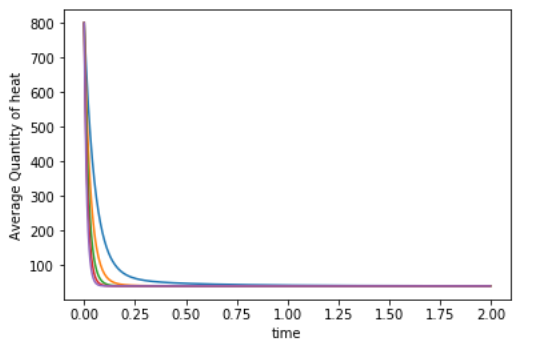
\includegraphics[width=\textwidth]{images/Barabasi-highest-degree.png}
        %		%\caption{$x=0.1, t=0$}
        %		%\label{gridt0x01}
        %	\end{subfigure}~
        %	\begin{subfigure}[b]{0.45\textwidth}
        %		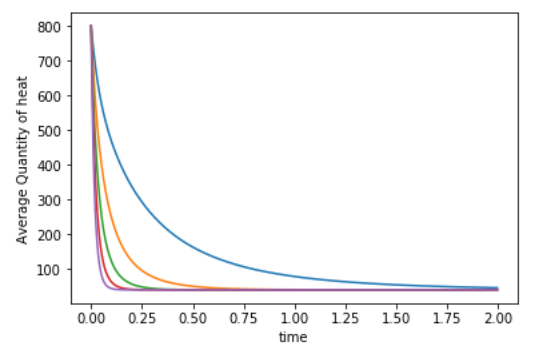
\includegraphics[width= \textwidth]{images/barabasi-random-selection.png}
        %		%\caption{$x=0.1, t=0.5$}
        %		%\label{gridt05x01}
        %	\end{subfigure}
        %	\caption{Illustration of the impact of the choice of the initial nodes from which diffusion starts. We consider Barabasi-Albert networks of $100$ nodes. The left plot corresponds to one in which the $5$ most important node according to degree centrality(hubs) are chosen. On the other hand, the plot at the right is as a result of random selection of initial nodes. }
        %	\label{}
        %\end{figure}
        \subsection{Diffusion on network with long-range interactions}
        The 'classical' case considers diffusion over a network where a substance under consideration say heat flows along the edges of the network. However, long range interactions during diffusive processes on networks are evident in real world situations. Such interactions result into superdiffussion on networks which has been modelled by various models that include the random walks with Levy flights (RWLF), model based on fractional diffusion equation (FDE), and many more. Recently, an elegant model has been put forward by Estrada \citep{estrada2017path} which accounts for longrange interactions by use of $k$-path Laplacian matrices resulting into a generalised diffusion process on networks.
        
        In this case, we consider diffusion on a graph where by both direct and long-range interactions are involved. One interesting study of long-range interactions is by Estrada on modelling epidermic spread in networks \citep{estrada2011epidemic}. Here, the long range interactions are considered to be nonrandom and depend on the social distances between individuals in the social network.
        Recently, work in \citep{estrada2012path} introduced a method of generalisation of the diffusion process on a given graph based on the k-path Laplacian operators $\mathbf{L}_k$ in which we consider the fact that the diffusive particle at a given node can hop to not only its nearest neighbours (captured by the classical Laplacian operator $\mathbf{L}$) but to any other nodes in the graph with a probability that decays with the increase of the shortest path distance between the current node where the particle is residing to the one it will hop to. Thus, for a diffusive node hopping to other nodes separated at a distance $k$ form its current location, such a diffusion process can be captured by replacing $\mathbf{L}$ in (\ref{dif-final-eqn}) by $\mathbf{L}_G$ in (\ref{infinite-dif}). That is 
        \begin{equation}
        \frac{d\boldsymbol{\phi}}{dt} = -\varepsilon \mathbf{L}_{G}\boldsymbol{\phi}, \quad \boldsymbol{\phi}(0) = \boldsymbol{\phi}_0 ,
        \label{gen-difeqn}
        \end{equation}
        where $L_G$ is the generalised Laplacian matrix. 
        
        
        We then consider the generalised diffusion on graph where interactions are both short-range and long-range. The long-range interactions are accounted for by use of $k$-path Laplacian matrices. Following this generalisation, Eqn.\ref{gen-difeqn} then becomes
        %    	    In accounting for indirect interaction, we consider the fact that longer paths contribute less compared to shorter ones. This is achieved by considering Equation \ref{dif-final-eqn} where $\mathbf{L}$ is any of the transformed $k$-path Laplacians given as
        
        \begin{equation}
        \frac{d\boldsymbol{\phi}}{dt} =  -\varepsilon \Big(\sum_{k=1}^{\Delta}c_k\mathbf{L}_{k} \Big) \boldsymbol{\phi}, \quad \boldsymbol{\phi}(0) = \boldsymbol{\phi}_0 ,
        \label{kgen-difeqn}
        \end{equation}
        
        \subsection{The Heat Kernel}
        As discussed earlier, diffusion of heat on a graph can be modelled by the equation 
        
        \begin{equation}
        \frac{d \phi}{dt} = -L \phi,
        \label{heateqn}
        \end{equation}
        where $L$ is either the Laplacian matrix or it's normalised version. 
        
        The heat kernel is the fundamental solution to the diffusion equation (\ref{heateqn}). It is obtained by exponentiating the Laplacian eigensystem and it is given by
        \begin{equation}
        H_t = exp(-Lt) 
        \label{kernel}
        \end{equation}
        It literally describes the flow of substance (heat) across edges (direct interactions) in the graph \citep{xiao2009graph}.
       
        When $t$ tends to zero, the kernel behaviour can be obtained from the Taylor's expansion of (\ref{kernel}) which is 
        \begin{equation}
        e^{-\mathbf{L}t} = \sum_{k=0}^{\infty} \frac{(-t)^k}{k!} \mathbf{L}^k = \mathbf{I} -\mathbf{L}t + \frac{\mathbf{L}^2 t^2}{2!} + \frac{\mathbf{L}^3 t^3}{3!}+ \cdots
        \end{equation}
        Thus,
        \begin{equation}
        \lim_{t\longrightarrow 0} \Big(e^{-\mathbf{L}t}\Big) = \mathbf{I} - \mathbf{L}t.
        \label{kerneltozero}
        \end{equation}
        It therefore implies that for $t$ tending to zero, the heat kernel depends on the local connectivity structure of the graph.
        On the other hand, as $t$ tends to infinity, we apply the spectral decomposition of Equation \ref{kernel} which is 
        \begin{equation}
        H_t = \mathbf{V} e^{(-\Lambda t)} \mathbf{V}^T =  \sum_{i=0}^n e^{(-\lambda_i t)} v_i v_i^T 
        \end{equation}
        where $\lambda_i$s are the eigenvalues of $L$ in a non-decreasing order $0=\lambda_1 \leq  \lambda_2 \leq, \cdots \leq \lambda_n$ and $v_i$ is the eigenvector corresponding to the eigenvalue $\lambda_i$. Thus,
        \begin{equation}
        \lim_{t\longrightarrow 0} \Big(e^{-\mathbf{L}t}\Big) = e^{(-\lambda_2 t)} v_2 v _2^T.
        \label{kernelinfinity}  
        \end{equation}
        From Equation \ref{kernelinfinity},its evident that for large $t$, the heat kernel behaviour is determined by the global structure of the graph. 
        \subsubsection{The Heat Kernel Invariants}
        \begin{enumerate}[1]
        	\item \textbf{Heat Kernel Trace}
        	
        	The trace of the heat kernel $Tr(H_t)$ is given by
        	\begin{equation}
        	Tr(H_t) = Tr(\mathbf{V} e^{(-\Lambda t)} \mathbf{V}^T)=Tr( e^{(-\Lambda t)} (\mathbf{V}^T \mathbf{V})) = Tr(e^{(-\Lambda t)})
        	%&=& Tr(\mathbf{V} (e^{(-\Lambda t)} \mathbf{V}^T)) \\
        	%&=& Tr( (e^{(-\Lambda t)} \mathbf{V}^T) \mathbf{V})\\
        	%&=& Tr( e^{(-\Lambda t)} (\mathbf{V}^T \mathbf{V})) \\
        	%&=& Tr(e^{(-\Lambda t)})
        	\end{equation}
%        	Like the trace of any other matrix, the trace of heat kernel is the summation of the main diagonal elements of the heat kernel matrix of a graph. 
        	Thus, the trace function of the heat kernel is given by 
        	\begin{equation}
        	Z(t) = Tr(H_t) = Tr(e^{(-\Lambda t)}) = \sum_{i=1}^{|V|} e^{-\lambda_i t},
        	\label{kerneltrace}
        	\end{equation}
        	where $\lambda_i$ is the eigenvalue of the normalised Laplacian matrix \cite{xiao2009graph}. 
        	For a connected graph ($\lambda_1 = 0$), Equation \ref{kerneltrace} can be written as 
        	\begin{equation}
        	Z(t) =  1+ e^{-\lambda_2 t} + e^{-\lambda_3t} + \cdots + e^{-\lambda_N t}
        	\end{equation}
        	Xiao \cite{xiao2009graph} developed a potential application of the trace formula as a basis for distinguishing different graphs based on the shape of the curves obtained by plots of the trace of the heat kernel as a function of time. Let us consider $3$ simple graphs namely a star, path and $2$-regular graph of size $10$. Fig shows the plot heat kernel trace against time for the three graphs.
        	
        	\begin{figure}[H]
        		\centering
        		\begin{subfigure}[b]{0.45\textwidth}
        			\includegraphics[width= \textwidth]{images/kernel-graphs.pdf}
        			\caption{}
        			\label{kernelgraphs}
        		\end{subfigure}~
        		\begin{subfigure}[b]{0.45\textwidth}
        			\includegraphics[width= \textwidth]{images/Trace-kernel-plot}
        			\caption{}
        			\label{plot-kernel}
        		\end{subfigure}\\
        		\begin{subfigure}[b]{0.45\textwidth}
        			\includegraphics[width= \textwidth]{images/mellin-s-2.png}
        			\caption{}
        			\label{starpathmellins2}
        		\end{subfigure}~
        		\begin{subfigure}[b]{0.45\textwidth}
        			\includegraphics[width= \textwidth]{images/mellin-s-3.png}
        			\caption{}
        			\label{starpathmellins3}
        		\end{subfigure}
        	\caption{(\subref{kernelgraphs}) are the three graphs used for heat kernel analysis. (\subref{plot-kernel}) plot of the heat kernel trace against time for star (blue), path (orange) and regular(green) graphs. Figures (\subref{starpathmellins2}) and (\subref{starpathmellins3}) are the plots of trace function against time for the $3$ graphs based on the Mellin transforms of the $k$-Laplacians for $s=2$ and $s=3$ respectively.}
        	\end{figure}
            From (\subref{plot-kernel}), we observe that since the $3$ graphs are different in terms of structure, the curves too take on different shapes. It is evident that since path and $2$-regular graphs have similar topologies, their corresponding graphs are close to each other while for star graph, its curve has a deeper trough. 
            On comparing the plots for $s=2$ and $s=3$, we observe drastic shift in the curves for the former than the latter in comparison with the plot for the normal graph Laplacian in Fig.(\subref{plot-kernel}).
            
            \item \textbf{Zeta function}
            
            The Zeta function associated with the Laplacian eigenvalues is obtained by exponentiating and summing the reciprocal of the non-zero Laplacian eigenvalues. It is thus defined by
            \begin{equation}
            \zeta(s) = \sum_{\lambda_i \neq 0} \lambda_i ^{-s}.
            \end{equation} 
            Xiao \cite{xiao2009graph} established a relationship between the zeta function and the heat kernel trace by use of the Mellin transform. For a function $f(t)$, it's Mellin transform is given by
            \begin{equation}
            F(s) = \int_{0}^{\infty} t^{s-1} f(t) dt.
            \end{equation}
            Taking a function $f(t)=e^{-\lambda_i t}$, applying the Mellin transform gives 
            \begin{equation}
            \lambda_i ^{-s} = \frac{1}{\Gamma(s)} \int_{0}^{\infty} t^{s-1} e^{-\lambda_i t} dt,
            \label{exponentlambda}
            \end{equation}
            where $\Gamma(s)$ is the gamma function defined as 
            \begin{equation}
            \Gamma(s) = \int_{0}^{\infty} t^{s-1} e^{-t} dt
            \end{equation}.
            On summation for all non-zero eigenvalues of the Laplacian, Equation \ref{exponentlambda} becomes
            \begin{equation}
            \zeta(s) = \sum_{\lambda_i \neq 0} \lambda_i ^{-s} = \frac{1}{\Gamma(s)} \int_{0}^{\infty} t^{s-1} \sum_{\lambda_i \neq 0} e^{-\lambda_i t} dt
            \label{label-kernel}
            \end{equation}
            The heat kernel trace can be also expressed as 
            \begin{equation}
            Tr(h_t) = C + \sum_{\lambda_i \neq 0} e^{-\lambda_i t}
            \label{kernelexp2},
            \end{equation}
            where $C$ is the multiplicity of zero eigenvalues of the Laplacian that is the number of connected components of a graph.
            Substituting Equation \ref{kernelexp2} into Equation 
            \ref{label-kernel} gives
            \begin{equation}
            \zeta(s) = \frac{1}{\Gamma(s)} \int_{0}^{\infty} t^{s-1} \left \{ Tr(h_t)-C \right \} dt.
            \end{equation}
            Thus the zeta function is related to the moments of the heat kernel trace. It is the moment generating function and thus a way of characterising the shape of the heat kernel trace.
          \item \textbf{Derivative of Zeta Function at the Origin}
          
        	The derivative or slope of the zeta function at the origin is another characterisation of the heat kernel trace second to the zeta function which measures it's shape. Writing the Zeta function in terms of natural exponential we have
        	\begin{equation}
        	\zeta(s) = \sum_{\lambda_i \neq 0} \lambda_{i} ^{-s} = \sum_{\lambda_i \neq 0} e^{-s \ln \lambda_i}.
        	\end{equation}
        	Thus, the derivative is given by
        	\begin{equation}
        	\zeta'(s) = \sum_{\lambda_i \neq 0} \{-\ln \lambda_i\}
        	e^{-s \ln \lambda_i}
        	\end{equation}
        	so, the derivative at the origin is 
        	\begin{equation}
	        \zeta'(s) = -\sum_{\lambda_i \neq 0}\ln \lambda_i
        	\end{equation}
        	\item \textbf{Heat Content}
        	
        	The heat content is defined as the sum of the entries of the heat kernel matrix of a graph. Its given by
        	\begin{equation}
        	Q(t) = \sum_{u \in V} \sum_{v i\in V} h_{t}(u,v)
        	\end{equation}
        	Substituting for $h_t(u,v)$ gives
        	\begin{equation}
        	Q(t) = \sum_{p \in V} \sum_{q i\in V} \sum_{k=1}^{\arrowvert V\arrowvert} e^{(-\lambda_{k} t)} v_{k}(p) v_{k}(q),
        	\end{equation}
        	which can be expanded into a polynomial in time as in \citep{mcdonald2002diffusions}
        	\begin{equation}
        	Q(t) = \sum_{m=0}^{\infty} q_m t^m
        	\end{equation}
        \end{enumerate}
    
        \subsection{Generalised Heat kernel}
        In the previous section, we have discussed the heat kernel for diffusion process that occurs through direct interactions between nearest neighbours in the network. In this section however, we consider the fact that in many observed real-world process, it is observed that interactions do not only occur among nearest neighbours but also among non-nearest which we term as the long range interactions. The heat equation in this case is based the the concept of $k$-path Laplacian introduced by Estrada \citep{estrada2012path} and is given by
        
        \begin{equation}
        \frac{d\boldsymbol{\phi}}{dt} =  -\varepsilon L_{G} \boldsymbol{\phi}, \quad \boldsymbol{\phi}(0) = \boldsymbol{\phi}_0 ,
        \label{genheateq}
        \end{equation}
        where
        \begin{equation}
        L_{G} =  \Big(\sum_{k=1}^{\Delta}c_k\mathbf{L}_{k} \Big) = c_{1}L_{1} + c_{2}L_{2} + \cdots + c_{\Delta}L_{\Delta}, 
        \label{}
        \end{equation}
        where $1 \leq \Delta \leq d_{max}$ and $c_k$ are the coefficients. As discussed earlier, 
        the coefficients $c_k$  are chosen in a way that as distance $k$ increases, the long range effect is weakened. Some of the common expressions for coefficients $c_k$ are $c_1 =1, c_{k\geq 2} = e^{-s k}$, $ c_{k\geq 2} =k^{-s}$ which depict physical influence while $c_k = kx^{k-1}$ for the social influence.
        
        The heat kernel $H_{Gt}$ of the generalised diffusion process which we refer to as the generalised heat kernel, the fundamental solution to eqn.\ref{genheateq} is given by 
        \begin{equation}
        H_{Gt} = e^{-L_{G}t},
        \end{equation}
        which on expansion can be written as 
        \begin{equation}
        H_{Gt} = e^{-t(c_{1}L_{1} + c_{2}L_{2} + \cdots + c_{\Delta}L_{\Delta})},
        \end{equation}
        where $L_1, L_2, \cdots, L{\Delta}$ are the matrices, known as $k$-path Laplacian matrices, which are obtained by considering hops of length $k=1,2,\cdots, \Delta$ respectively. At $k=1$, we recover the normal heat kernel in eqn.\ref{kernel}.
        \subsection{Trace of the Generalised Heat Kernel}
        The trace of the generalised heat kernel is therefore given by
        \begin{equation}
        Z_{G}(t) = Tr(H_{Gt}) = \sum_{i=1}^{|V|} e^{-\lambda_{iG} t}.
        \label{Genkerneltrace}
        \end{equation}
        Alternatively, Eqn. \ref{gen-difeqn} can be written as 
        \begin{equation}
        Z_{G}(t) =  1+ e^{-\lambda_{2G} t} + e^{-\lambda_{3G}} + \cdots + e^{-\lambda_{NG} t}
        \end{equation}
        Let us consider two toy examples to illustrate the variation of the trace generalised heat kernel with time.
         \begin{figure}[H]
         	\centering
         	\begin{subfigure}[b]{0.35\textwidth}
         		\includegraphics[width= \textwidth]{images/kenel-toymodel.pdf}
         		\caption{}
         		\label{keneltoymodel1}
         	\end{subfigure}~
         	\begin{subfigure}[b]{0.35\textwidth}
         		\includegraphics[width= \textwidth]{images/diffusion-graph.pdf}
         		\caption{}
         		\label{keneltoymodel2}
         	\end{subfigure} 
         	\caption{(\subref{keneltoymodel1}) is a simple network of size $5$ and (\subref{keneltoymodel2}) is a simple network of size $10$}.
         	\label{}
         \end{figure}

		\begin{figure}[H]
			\centering
			\begin{subfigure}[b]{0.45\textwidth}
				\includegraphics[width= \textwidth]{images/model-1-mellin.png}
				\caption{}
				\label{model1-mellin}
			\end{subfigure}~
			\begin{subfigure}[b]{0.45\textwidth}
				\includegraphics[width= \textwidth]{images/model-2-mellin.png}
				\caption{}
				\label{model2-mellin}
			\end{subfigure} 
		\end{figure}
		   \begin{figure}[H]
		    \begin{subfigure}[b]{0.45\textwidth}
		    	\includegraphics[width= \textwidth]{images/model-1-klap.png}
		    	\caption{}
		    	\label{model1-kpath}
		    \end{subfigure}~
		    \begin{subfigure}[b]{0.45\textwidth}
		    	\includegraphics[width= \textwidth]{images/model-2-klap.png}
		    	\caption{}
		    	\label{model2-kpath}
		    \end{subfigure}
			\caption{Figures (\subref{model1-mellin}) and (\subref{model2-mellin}) are plots of trace function of the generalised Laplacian matrix against time for graphs (\ref{keneltoymodel1}) and (\ref{keneltoymodel2}) respectively. On the other hand, figures in the lower row that is (\subref{model1-kpath}) and (\subref{model2-kpath}) are plots for the trace function for $k$-path Laplacian matrices ($L_1, L_2,\cdots, L_{\Delta}$) for graphs (\ref{keneltoymodel1}) and (\ref{keneltoymodel2}) respectively  }
			\label{}
		\end{figure}
	  The Mellin transforms of the $k$-path Laplacian matrices is one of ways used to account for long range interactions in networks. For the above simulations, we consider the exponents ranging from $2$ to $4$. In both cases, at $t=0$, the value of the trace function is equal to the size of the eigenvalues as each exponential term, $e^{\lambda_{iG}t} = 1$.  We also observe that as the exponent $s$ increases, the corresponding curve approaches that of the combinatorial Laplacian. This is based on the fact that the strength of the longrange interactions are controlled by the exponent, $s$ in such a way that the larger the value of $s$, the weaker the interactions. Interestingly, for $s=2$ in both figures (\subref{model1-mellin}) and (\subref{model2-mellin}), the trace of the heat kernel has a deeper trough compared to others. This can be explained by the superdiffusion that is always manifested at $s=2$ as discussed in the previous sections.
	  
	  Let us then focus on the plots for the trace function for the individual $k$-path Laplacians against time. Figure (\subref{model1-kpath}) corresponds to the simple graph in (\ref{keneltoymodel1}). We observe that there is a clear distinction for the trace functions of each of the $3$-path Laplacian matrices namely $L_1$, $L_2$, and $L_3$. For $k=1$ which is the combinatorial Laplacian, the curve has a deeper trough followed by $k=2$ and lastly $k=3$. This distinction in curves is possibly based on the change in eigenvalues for each of the $k$-path Laplacian following a decreasing of this format: $\lambda_i(L_1) \geq \lambda_i(L_2) \geq \lambda_i(L_3)$. On the other hand, however, Figure (\subref{model2-kpath}) shows a slightly different trend from what we observe in Figure (\subref{model1-kpath}) that is there is no clear distinction among the curves corresponding to different $k$-path Laplacian matrices. This is attributed to the fact that for some graphs, the eigenvalues for the $k$-path Laplacians do not necessarily follow a decreasing order as explained earlier.
	  
	  \subsection{Zeta function of the Generalised Zeta Function}
	  \begin{figure}[H]
	  	\centering
	  	\begin{subfigure}[b]{0.35\textwidth}
	  		\includegraphics[width= \textwidth]{images/zeta-laplace.png}
	  		\caption{}
	  		\label{zeta-laplace}
	  	\end{subfigure}~
	  	\begin{subfigure}[b]{0.35\textwidth}
	  		\includegraphics[width= \textwidth]{images/zeta-mellin.png}
	  		\caption{}
	  		\label{zeta-mellin}
	  	\end{subfigure} 
	  	\caption{Illustration of the Zeta function of the graph in Fig.~\ref{keneltoymodel1} against exponent $\delta$. (\subref{zeta-laplace}) corresponds to the Laplace transform of the graph Laplacian with $\lambda = 1.5, 2,$ and $2.5$. (\subref{zeta-mellin}) corresponds to the Mellin transform of the graph Laplacian with $s = 2, 3,$ and $4$. }
	  	\label{}
	  \end{figure}
  
      \begin{figure}[H]
      	\centering
      	\begin{subfigure}[b]{0.35\textwidth}
      		\includegraphics[width= \textwidth]{images/zeta-laplace2.png}
      		\caption{}
      		\label{zeta-laplace}
      	\end{subfigure}~
      	\begin{subfigure}[b]{0.35\textwidth}
      		\includegraphics[width= \textwidth]{images/zeta-mellin2.png}
      		\caption{}
      		\label{zeta-mellin}
      	\end{subfigure} 
      	\caption{Illustration of the Zeta function of the graph in Fig.~\ref{keneltoymodel2} against exponent $\delta$. (\subref{zeta-laplace}) corresponds to the Laplace transform of the graph Laplacian with $\lambda = 1.5, 2,$ and $2.5$. (\subref{zeta-mellin}) corresponds to the Mellin transform of the graph Laplacian with $s = 2, 3,$ and $4$. }
      	\label{}
      \end{figure}
	  
	  \subsection{Comparison with Complete Graph based on Trace of the diffusion kernel}
	  \begin{figure}[H]
	  	\centering	\begin{subfigure}[b]{0.32\textwidth}
	  		\includegraphics[width= \textwidth]{images/complete_5.pdf}
	  		\caption{G}
	  		\label{G}~
	  	\end{subfigure}	  	\begin{subfigure}[b]{0.30\textwidth}
	  		\includegraphics[width= \textwidth]{images/cycle-khop.pdf}
	  		\caption{G1}
	  		\label{G1}
	  	\end{subfigure}~
	  	\begin{subfigure}[b]{0.35\textwidth}
	  		\includegraphics[width= \textwidth]{images/kenel-toymodel.pdf}
	  		\caption{G2}
	  		\label{G2}
	  	\end{subfigure} \\
	  	\begin{subfigure}[b]{0.35\textwidth}
	  		\includegraphics[width= \textwidth]{images/G3-khop.pdf}
	  		\caption{G3}
	  		\label{G3}
	  	\end{subfigure}~
	  	\begin{subfigure}[b]{0.35\textwidth}
	  		\includegraphics[width= \textwidth]{images/G4-khop.pdf}
	  		\caption{G4}
	  		\label{G4}
	  	\end{subfigure}
	  	\caption{The five graphs of size $5$. (\subref{G2}) is the complete graph,$K_5$ whose trace function is to be compared with that of the other $4$ graphs.}
	  	\label{}
	  \end{figure}
 
	  \begin{figure}[H]
	  	\centering
	  	\begin{subfigure}[b]{0.45\textwidth}
	  		\includegraphics[width= \textwidth]{images/complete-L1.png}
	  		\caption{}
	  		\label{completeL1}
	  	\end{subfigure}~
	  	\begin{subfigure}[b]{0.45\textwidth}
	  		\includegraphics[width= \textwidth]{images/s2-graphcomp.png}
	  		\caption{}
	  		\label{completeMellins3}
	  	\end{subfigure} \\
  	    \begin{subfigure}[b]{0.45\textwidth}
  	    	\includegraphics[width= \textwidth]{images/s3-graphcomp.png}
  	    	\caption{}
  	    	\label{completeL1}
  	    \end{subfigure}~
  	    \begin{subfigure}[b]{0.45\textwidth}
  	    	\includegraphics[width= \textwidth]{images/s4-graphcomp.png}
  	    	\caption{}
  	    	\label{completeMellins3}
  	    \end{subfigure}
  	\end{figure}
      Figure \ref{completeL1} is a plot of the trace function of the graph Laplacian against time for a complete graph,G (blue) and other graphs $G1$(orange), $G2$(green), $G3$(red), and $G4$(purple). To the right, is a plot of the trace function of the Mellin transformed Laplacian matrix at $s=3$ against time. We observe that the two plots follow a similar shape, however, plot in Figure \ref{completeMellins3}, the curves for graphs $G1$,$G2$, $G3$, and $G4$ get closer to the curves corresponding to the complete graph$G$. This can loosely be explained by the longrange interactions involved that result into a flow of information closer to that of a complete graph.
  
	  
        \subsubsection{Simulations of diffusion on lattice}
         We consider a 2-dimensional discrete grid in which each point is connected to 8 of its nearest neighbours. Initially, we assign heat quantities to all the points on the grid and then we investigate how the diffusion process occurs and at each time $t$. 
   
         Let us take a $20$ by $20$ grid on which we assigned heat quantities of amounts $5$, $7$ and $10$ to a few points and the rest are assigned zero. The diffusion on the lattice through direct interactions only as well as through both direct and indirect interactions by using the Social distance concept, Laplace and Mellin tranforms.
         
         \begin{enumerate}[i)]
         	\item Diffusion on lattice through Direct interactions only
         	\begin{figure}[!h]
         		\centering
         		\begin{subfigure}[b]{0.25\textwidth}
         			\includegraphics[width=\textwidth]{images/grid-t0-x0.png}
         			\caption{$t=0$}
         			\label{gridt0x0}
         		\end{subfigure}~
         		\begin{subfigure}[b]{0.25\textwidth}
         			\includegraphics[width= \textwidth]{images/grid-t05-x0.png}
         			\caption{$t=0.5$}
         			\label{gridt05x0}
         		\end{subfigure}~
         		\begin{subfigure}[b]{0.25\textwidth}
         			\includegraphics[width= \textwidth]{images/grid-t3-x0.png}
         			\caption{$t=3.0$}
         			\label{gridt3x0}
         		\end{subfigure}~
         		\begin{subfigure}[b]{0.25\textwidth}
         			\includegraphics[width= \textwidth]{images/grid-t5-x0.png}
         			\caption{$t=5.0$}
         			\label{gridt5x0}
         		\end{subfigure}
         		\caption{Sample illustrations for progression of diffusion over a $20 \times 20$ lattice where specific regions are assigned particular heat quantities which in turn spread to other regions of low heat quantities through interactions along links in the network.}
         		\label{gridx0}
         	\end{figure}
         
            
         	
         	\item Diffusion on lattice through both direct and indirect interactions.
         	Considering a similar lattice with initial heat quantity assignments as in the directed case discussed before, we account for the diffusion process where interactions among nodes occurs through both direct and indirect interactions.
         	
         	As discussed previously, long-range interactions can be accounted for by using various techniques as illustrated by the following illustrations.
         	\begin{enumerate}[a)]
         		\item Long range interactions using social distance 
         		Taking $x=0.1$ and $x=0.2$.
         		\begin{figure}[!h]
         			\centering
         			\begin{subfigure}[b]{0.25\textwidth}
         				\includegraphics[width=\textwidth]{images/grid-t0-x01.png}
         				\caption{$t=0$}
         				\label{gridt0x01}
         			\end{subfigure}~
         			\begin{subfigure}[b]{0.25\textwidth}
         				\includegraphics[width= \textwidth]{images/grid-t05-x01.png}
         				\caption{$t=0.5$}
         				\label{gridt05x01}
         			\end{subfigure}~
         			\begin{subfigure}[b]{0.25\textwidth}
         				\includegraphics[width= \textwidth]{images/grid-t3-x01.png}
         				\caption{$t=3.0$}
         				\label{gridt3x01}
         			\end{subfigure}~
         			\begin{subfigure}[b]{0.25\textwidth}
         				\includegraphics[width= \textwidth]{images/grid-t5-x01.png}
         				\caption{$t=5.0$}
         				\label{gridt5x01}
         			\end{subfigure}
         		   \label{gridx01}
         		\end{figure}
         		
         		\begin{figure}[!h]
         			\centering
         			\begin{subfigure}[b]{0.25\textwidth}
         				\includegraphics[width=\textwidth]{images/grid-t0-x02.png}
         				\caption{$t=0$}
         				\label{gridt0x02}
         			\end{subfigure}~
         			\begin{subfigure}[b]{0.25\textwidth}
         				\includegraphics[width= \textwidth]{images/grid-t05-x02.png}
         				\caption{$t=0.5$}
         				\label{gridt05x02}
         			\end{subfigure}~
         			\begin{subfigure}[b]{0.25\textwidth}
         				\includegraphics[width= \textwidth]{images/grid-t3-x02.png}
         				\caption{$t=3.0$}
         				\label{gridt3x02}
         			\end{subfigure}~
         			\begin{subfigure}[b]{0.25\textwidth}
         				\includegraphics[width= \textwidth]{images/grid-t5-x02.png}
         				\caption{$t=5.0$}
         				\label{gridt5x02}
         			\end{subfigure}\\
         			\vspace{0.25cm}
         			\begin{subfigure}[b]{0.60\textwidth}
         				\includegraphics[width= \textwidth]{images/colour-bar-grid.png}
         			\end{subfigure}
         			\caption{Illustrations for diffusion over a grid with long-range interactions accounted for by the social distance technique. The upper row corresponds to diffusion with conductance $x=0.1$ while lower row corresponds to results obtained $x=0.2$. The intensity of heat follows a color grid where by red implies higher intensity followed by yellow and blue implies low heat intensities.}
         			\label{gridlongrange}
         		\end{figure}
         		
         		At $t=0$, diffusion on the grid starts off with $3$ strong regions having high quantities of heat as observed from figures \ref{gridx0}, and \ref{gridlongrange} which correspond to diffusion with direct interactions only and diffusion with conductance $x = 0.1$ and $0.2$ respectively. As the diffusion process continues, we see that at $t=0.5$, strong heat points can still be spotted for direct interactions, relatively strong points in $x=0.1$ and almost complete diffusion in $x=0.2$. We can also observe that by $t=2.0$, heat is uniformly distributed across the grid for $x=0.1$ and $x=0.2$. However, for the case of direct interactions (Fig.\ref{gridt5x0}) diffusion is still ongoing and we can notice strong heat points at the centre of the grid. Following the sequences in the figures, we can conclude that as $x$ (i.e increase in intensity of long range interactions), the diffusion process goes faster and equilibrium across the grid is reached faster as observed in the above simulations where for $x=0.2$, $x=0.1$ equilibrium is reached by $t=3$ while for $x=0$, equilibrium is not yet reached by then.
         		 
         		\item Longrange interactions using Laplace Transforms
         		\begin{figure}[!h]
         			\centering
         			\begin{subfigure}[b]{0.25\textwidth}
         				\includegraphics[width=\textwidth]{images/laplace-x1-t0.png}
         				\caption{$t=0$}
         				\label{laplacet0x01}
         			\end{subfigure}~
         			\begin{subfigure}[b]{0.25\textwidth}
         				\includegraphics[width= \textwidth]{images/laplace-x1-t05.png}
         				\caption{$t=0.5$}
         				\label{laplacet05x01}
         			\end{subfigure}~
         			\begin{subfigure}[b]{0.25\textwidth}
         				\includegraphics[width= \textwidth]{images/laplace-x1-t3.png}
         				\caption{$t=3.0$}
         				\label{laplacet3x01}
         			\end{subfigure}~
         			\begin{subfigure}[b]{0.25\textwidth}
         				\includegraphics[width= \textwidth]{images/laplace-x1-t5.png}
         				\caption{$t=5.0$}
         				\label{laplacet5x01}
         			\end{subfigure}
         		\caption{Illustration for diffusion on the lattice with both direct and long range interactions. These longrange interactions are accounted for by Laplace transforms given by Equation \ref{laplacetransform}  with $\lambda=1$.}
         		\end{figure}
         		
         		\item Longrange interactions using Mellin Transforms of the $k$-Laplacian matrices.
         		\begin{figure}[!h]
         			\centering
         			\begin{subfigure}[b]{0.25\textwidth}
         				\includegraphics[width=\textwidth]{images/mellin-x2-t0.png}
         				%\caption{$x=0, t=0$}
         				%\label{gridt0x0}
         			\end{subfigure}~
         			\begin{subfigure}[b]{0.25\textwidth}
         				\includegraphics[width= \textwidth]{images/mellin-x2-t05.png}
         				%\caption{$x=0, t=0.5$}
         				%\label{gridt05x01}
         			\end{subfigure}~
         			\begin{subfigure}[b]{0.25\textwidth}
         				\includegraphics[width= \textwidth]{images/mellin-x2-t3.png}
         				%\caption{$x=0, t=3.0$}
         				%\label{gridt3x01}
         			\end{subfigure}~
         			\begin{subfigure}[b]{0.25\textwidth}
         				\includegraphics[width= \textwidth]{images/mellin-x2-t5.png}
         				%\caption{$x=0, t=5.0$}
         				%\label{gridt5x01}
         			\end{subfigure}
         			\caption{}
         			%\label{gridatx0}
         		\end{figure}
         	    \begin{figure}[!h]
         	    	\centering
         	    	\begin{subfigure}[b]{0.25\textwidth}
         	    		\includegraphics[width=\textwidth]{images/mellin-x4-t0.png}
         	    		%\caption{$x=0, t=0$}
         	    		%\label{gridt0x0}
         	    	\end{subfigure}~
         	    	\begin{subfigure}[b]{0.25\textwidth}
         	    		\includegraphics[width= \textwidth]{images/mellin-x4-t05.png}
         	    		%\caption{$x=0, t=0.5$}
         	    		%\label{gridt05x01}
         	    	\end{subfigure}~
         	    	\begin{subfigure}[b]{0.25\textwidth}
         	    		\includegraphics[width= \textwidth]{images/mellin-x4-t3.png}
         	    		%\caption{$x=0, t=3.0$}
         	    		%\label{gridt3x01}
         	    	\end{subfigure}~
         	    	\begin{subfigure}[b]{0.25\textwidth}
         	    		\includegraphics[width= \textwidth]{images/mellin-x4-t5.png}
         	    		%\caption{$x=0, t=5.0$}
         	    		%\label{gridt5x01}
         	    	\end{subfigure}
         	    	\caption{Illustrations of diffusion process on the lattice allowing for both direct and longrange interations. The latter are accounted for using Mellin transforms of the $k$-Laplacian matrices as in Equation.~\ref{mellin-transforms}. The top row corresponds to the case for which $s=2$ and the bottom row corresponds to case $s=4$.}
         	    	\label{mellintransformsfig}
         	    \end{figure}
         	 For the case of Mellin transforms, we observe that rate of diffusion is quite faster at $k=2$(upper row) than at $k=4$(lower row).This is due to the fact that at $k<3$, super diffusion occurs, however normal diffusion occurs when $k>3$ as shown in lower row of Fig.\ref{mellintransformsfig}.
         	\end{enumerate}
         \end{enumerate}
         
  
\newpage
\section{Image segmentation}
Image segmentation is defined as the problem of localising regions of an image relative to content such as image homogeneity. There are various algorithms that perform image segmentation based on specific content localisation such as intensity, color, texture, etc.
It is important to note a good image segmentation algorithm must perform fast computation and editing, produce arbitrary segmentation with enough interaction as well as producing intuitive images. 

Graph theory concepts are often applied in developing a number of image segmentation algorithms such as graph cuts algorithms, the intelligent scissor algorithm, the random walker algorithm, among others.

\subsection{Image segmentation based on Random Walks}
A random walk (also known as drunkard's walk) is a stochastic process that describes a path that consists of a succession of random steps on some mathematical space. An example of a random walk on a graph can be described as  in the following way:
%Suppose we have a number line representing stations in range $1$ to $5$. Take a drunkard starting at station $3$ (middle), with probability $1/2$, he can either move to station $2$ or to station $4$. on arriving to any of the chosen station, a similar decision is made on which station to visit next and the process goes on until the drunkard reaches his final destination (say it is station $5$). A walk covering the visited stations is what we refer to as the random walk.
Suppose a walker starts off a given node $i$ and then moves to one of the neighbouring nodes of $i$, say $j$, with a uniform probability. Once at $j$, the walker again moves to the next node following a similar process until the stopping node. the sequence of these randomly visited nodes is referred to as the random walk.

There are various types of random walks, however, for the work we consider lattice random walkers that is to say random walkers that occur on on the lattice.

Here, we study the application of random walker on 2-d lattice to the segmentation of images. 
  
\subsection{Random Walks and Electric potential}
Let's consider a graph $G=(V,E)$ with two nodes, $a$ and $b$, selected as traps with a score of $0$ and $1$ for hitting nodes $a$ and $b$ respectively. So for any other node $x$, the probability $p(x)$ of reaching node $b$ given that the walker started at node $x$ is given by
\begin{equation}
p(x) = \frac{1}{d_x} \sum_{y, y \in N(x)} p(y),
\label{eqnp1}
\end{equation}
where $N(x)$ denotes the neighbours of $x$.
\begin{equation}
p(a) = 0
\label{eqnp2}
\end{equation}
\begin{equation}
p(b) = 1
\label{eqnp3}
\end{equation}

We then consider a graph $G=(V,E)$ as an electrical network which consists of connected wires. The vertices  represent the intersections of the wires in the circuit such that $v_x$ is the voltage at a given vertex $v \in V$. On the other hand, the edges represent the resistors along the wires such that for each edge $x,y \in E$ is a resistor of resistance $r_{x,y}$.
Suppose we set the resistances $r_{x,y}$ for any pairs of nodes in graph to $1$ Ohm and set the voltages of vertices $a$ and $b$ to $0$ and $1$ respectively that is 
\begin{equation}
v(a) = 0
\label{eqnv1}
\end{equation}
\begin{equation}
v(b) = 1
\label{eqnv2}
\end{equation}
 

By Ohm's law the current flowing through vertices $x$ and $y$ is given by
\begin{equation}
i_{x,y} = v(x) -v(y) \quad \forall x\neq y\neq b, \quad x,y \in E
\end{equation}
Applying Kirchoff's law, we have
\begin{equation}
\sum_{x~y} i_{x,y} =0 , \quad \sum_{y,x~y} v(x) -v(y)  =0,
\end{equation}
which gives
\begin{equation}
v(x) = \frac{1}{d_x} \sum_{y, y \in N(x)} v(y)
\label{eqnv3}
\end{equation}

We observe that system of equation of the probabilities in (\ref{eqnp1},\ref{eqnp2},\ref{eqnp3}) and that of the voltages (\ref{eqnv1},\ref{eqnv2},\ref{eqnv3}) follow the same law. That is to say they are both harmonic functions and satisfy the following properties
\begin{enumerate}
	\item Mean value property
	Let us consider simpler example of one dimension case. Let $A$ be the set of points $A=\{0,1,2,\cdots,N\}$ and let $B$ be the set of  boundary points $B=\{ 0,N\}$ and $C$ be the set of interior points $C = \{ 1,2,\cdots, N-1\}$. So the function $f(x)$ defined on $A$ is harmonic if it satisfies the mean value property given as
	\begin{equation}
	f(x) = \frac{f(x+1) + f(x-1)}{2}
	\label{meanprop}
	\end{equation}
From (\ref{eqnp1}) and (\ref{eqnv3}), we observe both functions $p$ and $v$ satisfy the mean value property in (\ref{meanprop}) since for any node other than $a$ or $b$, the value of the function at that node is the average of the values of its neighbours. 

In addition, both functions have the same values at the boundary that is at nodes $a$ and $b$.
  \item Maximum principle
  A harmonic function $f(x)$ defined on $A$ is said to satisfy the maximum principle if minimum and maximum values are attained only at the boundary. For functions $v$ and $p$, we can observe from (\ref{eqnp2},\ref{eqnp3}) and (\ref{eqnv1},\ref{eqnv2}) respectively that the maximum principle holds.
  
  \item Uniqueness Principle
  
  If $f(x)$ and $g(x)$ are harmonic functions on $A$ such that $f(x)=g(x)$ on $B$, then $f(x)=g(x)$ for all $x$. Following from previous discussions, $v(x)$ and $p(x)$ follow the uniqueness principle which implies that the two functions are equal. This therefore implies that the probability of a random walker reaching a given labelled node $y$ given that the walker started at node $x$ is equal to the electric potential developed at node $x$ when node $y$ is set to a potential of $1$ volt. It is this similarity between random walks and electric potentials on graphs that was applied in the development of  image segmentation using random walker algorithm as we will explore in the next sections.
\end{enumerate}
	
\subsection{The Random walker Algorithm}
\subsubsection{Problem Formulation}
First, we represent the image as a weighted undirected graph (discrete object) where each pixel is represented as a node and each node connected by weighted edges to either $4$ or $8$ of its nearest neighbours. The real-valued edge weights can be captured by various weighting functions. However, in this work we use a Gaussian weighting function which maps changes in pixel intensities to  the edge weights as given by
\begin{equation}
w_{i,j} = exp(-\beta (g_i -g_j)^2),
\label{edgeweights}
\end{equation}
where $\beta$ is a free parameter, $g_i$ is the intensity at pixel $i$.
To capture colour,filter coefficients, texture or any other desired image features, we can modify (\ref{edgeweights}). For instance, to capture colour, we replace $(g_i -g_j)^2$ with $\|g_i -g_j\|^2$  $ \forall e_{i,j} \in E$ \citep{grady2006random}.

Having represented the image as a graph and given user-defined seeds that represent regions of belonging to the desired objects, we obtain an interactive image segmentation by assigning each unseeded node or pixel to the seed to which a random walker starting at the unseeded node first reaches a particular seed. The random walker is biased by the edge weights to avoid crossing sharp intensity gradients for respect of boundary objects.

Suppose we have an image that we would like to segment into $K$ regions or objects that is to say a $k$-way image segmentation.
First, seeds are selected by user to represent the desired $k$ regions. The main task involves obtaining a $k$-tuples of probabilities with which a random walker starting at each unseeded node reaches the seeds. Each unseeded node is then assigned a label for the seed for which the largest probability was obtained. One approach to this problem would be simulation of the random walker process though unfortunately, the method would be infeasible for certain image segmentation problems of interest. Alternatively, work in \citep{grady2006random} indicates that the probability with which a random walker first reaches a given seed can be found as a solution to the Combinatorial Dirichlet problem  with boundary conditions at the location of the seed points with the seed in question set to $1$ as the rest of the seeds are set to $0$. With this approach, we can then analytically compute the desired probabilities as we will discuss in the next subsections. 
\subsubsection {Combinatorial Dirichlet Problem}
Dirichlet problem is the problem of finding a harmonic function subject to its boundary conditions. A harmonic function is a function that satisfies the Laplace equation
\begin{equation}
\nabla^2 u = 0,
\end{equation}
for a field $u$. The harmonic function that satisfies the boundary conditions minimises the Dirichlet integral
\begin{equation}
D[u]= \frac{1}{2} \int_{\Omega} |\nabla|^2 d\Omega,
\end{equation}
for region $\Omega$.\\
Let us consider an image represented as a graph G=(V,E) where nodes represent pixels while edges represent the neighbourhood among the pixels. The Combinatorial Laplacian matrix of the graph is defined as

\begin{equation}
L_{ij} = \begin{cases}
d_i & \text{if } i=j, \\
-w_{ij} & \text{if } v_i \text{ and } v_j \text{ are adjacent nodes},\\
0 & \text{otherwise,}
\end{cases}
\end{equation}
where $L_{i,j}$ is indexed by vertices $v_i$ and $v_j$.
The combinatorial formulation of the Dirichlet integral is 
\begin{equation}
D[x] = \frac{1}{2} x^T L x = \sum_{e_{ij} \in E} w_{ij} (x_i -x_j)^2.
\label{combDirichlet}
\end{equation}
A combinatorial harmonic is a function $x$ that minimises \ref{combDirichlet}.
\subsubsection{Implementation of Algorithm}
\begin{enumerate}
	\item Computing probabilities:
	
	With Graph $G=(V,E)$ representing the image to be segmented, partition the vertex set into two such that is $V_m$ and $V_u$ which are the seeded/marked and unseeded vertices respectively such that $V_m \bigcup V_u = V$ and $V_m \bigcap V_u = \emptyset$.
	Without loss of generality, we assume that the nodes in $L$ are arranged such that the seeded nodes are first followed by the unseeded ones. Then equation \ref{combDirichlet} can be written as 
	\begin{equation}
	D[x_u] = \frac{1}{2} \begin{bmatrix}
	x_m ^T x_m ^T
	\end{bmatrix} \begin{bmatrix}
	L_m & & B \\\\
	B^T & & L_u
	\end{bmatrix} \begin{bmatrix}
	x_m \\ \\
	x_u
	\end{bmatrix} = 
	\frac{1}{2}( x_m ^T L_m x_m + x_u ^T B^T x_m + x_u ^T L_u x_u),
	\end{equation}
	where $x_m$ and $x_u$ correspond to the potentials at the seeded and unseeded nodes respectively.
	Differentiating $D[x]$ with respect to $x_u$ and then finding the critical points gives  the following system of linear equations with $|V_u|$ unknowns
	\begin{equation}
	L_u x_u = -B^T x_m.
	\end{equation} 
	Let $x_i ^s $ be the probability of a random walker starting at node $v_i$ first reaches label $s$. Then for each label $s$ the probabilities with each unlabelled nodes first reach $s$ is given by
	\begin{equation}
	L_u x^s = -B^T m^s,
	\end{equation}
	and for all labels, we have 
		\begin{equation}
	L_u X = -B^T M,
	\label{finalprobs}
	\end{equation}
	where $X$ has $K$ columns taken by each $x^s$ and $M$ has columns given by each $m^s$.
	
	\item Assigning labels to unseeded nodes
	Having computed the probabilities for each unseeded nodes, we assign a label to each node for which the highest probability was obtained.
\end{enumerate}
\subsection{Possible application of Long range interactions to Image Segmentation}
We considered a possible application of long range interaction to segmentation of image based on random walks. This was implemented by replacing the Combinatorial Laplacian matrix $L$ in equation \ref{finalprobs}  with the the $k$-path Laplacian matrices to account for long range jumps of the random walker. However, the output obtained using this method was not a better image segmentation due to the fact that the long-range jumps do not take into account the localisation of objects in an image which results into less intuitive image segmentation. 

\newpage
\section{Laplacian Centrality of weighted Networks}
The centrality of a node is a measure of how important or central a node is with in a network. A variety of centrality measures have been introduced for undirected unweighted networks based on various definitions of importance of a node. These include: degree, closeness, betweenness, eigenvector and subgraph centralities \citep{freeman1978centrality,estrada2005subgraph}. Standard centrality measures i.e degree, closeness, and betweenness  were extended to weighted networks due to the fact that weighted networks provide more information about the network and therefore measures applied to these networks are of great importance \citep{newman2001scientific,barrat2004architecture,opsahl2009structure,opsahl2010node}. 
These standard centrality measures give information on either the local environment of a node (i.e degree centrality) or the global position of a node in the network (i.e closeness, betweenness and subgraph centralities). This implies that information about the intermediate (between local and global) environment of a node cannot be captured by any of the standard centralities, yet, such information is very useful in the study of real-world networks. For instance, quantifying the relative importance of a particular actor in a social network. It is for this reason that a new type of centrality known as the Laplacian centrality was introduced \citep{qi2012laplacian}. 


With Laplacian centrality measure, the importance of a node is determined by the ability of the network to respond to the deactivation  of the node from the network. In other words, it is a measure of the relative drop of Laplacian energy in the network due to the removal (or deactivation) of the node from the network. The drop of Laplacian energy with respect to node $v$ is determined by the number of $2$-walks that $v$ participates in the network \citep{qi2012laplacian}. 

\subsection{Laplacian energy of a network}
Let $G = (V,E,W)$ be a simple undirected weighted network with the vertex set $V(G) = \{v_1,v_2,\cdots, v_n\}$, edge set $E$, where each edge $e=(v_i,v_j)$ is attached with a weight $w_{ij}$. If there is no edge between $v_i$ and $v_j$, $w_{i,j}=0$. In addition, $w_{i,i} =0$ and $w_{i,j} = w_{j,i}$. We define 
\begin{eqnarray*}
	\mathbf{W(G)} = \begin{pmatrix}
		0 & w_{1,2} & \ldots  & w_{1,n} \\
		w_{2,1} & 0 & \ldots & w_{2,n} \\
		\vdots   & \vdots & \vdots & \vdots \\
		w_{n,1} & w_{n,2} & \ldots & 0 
	\end{pmatrix} \text{ and }
	\mathbf{X(G)} = \begin{pmatrix}
		x_1 & 0 & \ldots  & 0 \\
		0 & x_2 & \ldots & 0 \\
		\vdots   &\vdots & \vdots & \vdots \\
		0 & 0 & \ldots & x_n
	\end{pmatrix} ,
\end{eqnarray*}
where $x_i$ is the sum-weight of vertex $v_i$ given by $x_i = \sum_{j=1}^n w_{i,j} = \sum_{u \in N(v_i)} w_{v_i,u}$, where $N(v_i)$ is the neighborhood of $v_i$.
\begin{defn}[Weighted Laplacian matrix]
	The Laplacian matrix of a weighted network $G$ is the matrix $\mathbf{L(G)} = \mathbf{X(G)} - \mathbf{W(G)}$. 
\end{defn}
\begin{defn}[Laplacian Energy of a network]
	Let $G=(V,E,W)$ be a weighted network on $n$ vertices and $\lambda_1,\lambda_2, \ldots,\lambda_n$ be the eigenvalues of its Laplacian matrix. The Laplacian energy of $G$ is defined as 
	\begin{eqnarray*}
		E_L(G) = \sum_{i=1}^n \lambda_i ^2 .
	\end{eqnarray*} 
\end{defn}
As networks become larger, computing eigenvalues of the Laplacian matrix becomes very hard. We therefore, use the entries of the Laplacian matrix rather than its eigenvalues to compute the Laplacian energy of a network as given by Theorem \ref{theorem:1}.
\begin{thm}
	For any network $G=(V,E,W)$ on $n$ vertices whose vertex sum-weights are  
	
	$x_1,x_2, \ldots, x_n$ respectively, we have
	\begin{eqnarray}
	E_L(G) = \sum_{i=1}^n x_i^2 + 2 \sum_{i<j} w_{i,j}^2.
	\end{eqnarray}
	\label{theorem:1}
\end{thm}

\begin{cor}
	If $H$ is an arbitrary subgraph of a network $G$, then $E_L(H) \leq E_L(G)$. And equality holds if and only if $V(G)-V(H)$ is a set of isolated vertices.
	\label{cor:1}
\end{cor}

\subsection{Laplacian centrality for a vertex}
\begin{defn}
	If $G=(V,E,W)$ is a network with $n$ vertices $\{v_1,v_2,\ldots, v_n\}$. Let $G_i$ be the network obtained by deleting $v_i$ from $G$. The Laplacian centrality is given by
	\begin{eqnarray}
	C_L(v_i,G) = \frac{(\Delta E)_i}{E_L(G)} = \frac{E_L(G) - E_L(G_i)}{E_L(G)}
	\end{eqnarray} 
	\label{lapcentrality-undirected}
\end{defn}
For any vertex $v$, the denominator remains unchanged and from Corollary \ref{cor:1}, we can tell that $E_L(G) - E_L(G_i)$ is non-negative. We then focus on obtaining the expression for $(\Delta E)_i$. In order to obtain the graph theoretical descriptions of Laplacian centrality, we will study the $k$-walks (discussed in Chapter 2) for the weighted graph, specifically, for $k=2$. For better understanding of the weighted network concept, we represent a weighted network as an unweighted multigraph network by replacing each edge $e=(v_i,v_j)$ with $w_ij$ copies of multiedges. For instance, for a $2$-walk $v_1v_2v_3$ in a weighted network, the number of $2$-walks in its corresponding unweighted network is  $w_{v_1,v_2}w_{v_2,v_3}$. 

\begin{thm}
	Let $G=(V,E,W)$ be a weighted network of $n$ vertices ${v_1,v_2,\ldots,v_n}$. Let $G_i$ be the network obtained by deleting vertex $v$ from $G$, then the drop of Laplacian energy with respect to $v_i$ is
	\begin{eqnarray}
	(\Delta E)_i = E_L(G) -E_L(G_i) = 4 \cdot NW_2^C (v_i) + 2 \cdot NW_2^E (v_i) + 2 \cdot NW_2^M (v_i).
	\label{energychange}
	\end{eqnarray}
	where
	$NW_{2} ^C(v_i)$, $NW_{2} ^E(v_i)$, and $NW_{2} ^M(v_i)$ are closed $2$-walks containing vertex $v_i$, non-closed $2$-walks with vertex $v_i$ as one of the end points and non-closed $2$-walks with vertex $v_i$ as the middle point\citep{qi2012laplacian}.
	\label{thm2}
\end{thm}
%\subsection{Edge Centralities in Networks}
\subsection{Laplacian Centrality of a node of a Graph with long-range interactions}
In this section, we study the impact of long-range interactions in a graph on the Laplacian centrality of the nodes in the network. For example, let us consider a simple graph in Fig.\ref{toymodel}. We account for the long range interactions (shown by the brocken red edges) by the mellin transform($c_k = k^{-s}$) of the $k$-Laplacian matrices of the graph for $s=2$ as  visible in Fig.~\ref{graph-longrange}.

\begin{figure}[!h]
	\centering
	\begin{subfigure}[b]{0.3\textwidth}
		\includegraphics[width=\textwidth]{images/kenel-toymodel.pdf}
		\caption{}
		\label{toymodel}
	\end{subfigure}~
	\begin{subfigure}[b]{0.3\textwidth}
		\includegraphics[width= \textwidth]{images/graph-longrange-demo.pdf}
		\caption{}
		\label{graph-longrange}
	\end{subfigure}
	\caption{(\subref{toymodel}) is a simple graph. (\subref{graph-longrange}) is the mellin transformation of the graph in (\subref{toymodel}) with $s=2$.   }
	\label{}
\end{figure}

\begin{table}[H]
	\centering
	\caption{Laplacian Centralities of nodes with and without long range interactions}
	%\setlength{\tabcolsep}{16pt}
	%\scalebox{0.7}{
	\begin{tabular}{|l| c|c|c|}
		\hline 
		Node & Centrality without longrange & Centrality with longrange \\
		\hline
		1 & 0.2500 & 0.3175 \\
		2 & 0.6875 & 0.6712  \\
		3 & 0.5000 & 0.5185  \\
		4 & 0.4375 & 0.4702 \\
		5 & 0.5000 & 0.5185 \\
		\hline
	\end{tabular}
	\label{laplacian-longrange}
\end{table}
From the table, we observe that accounting for longrange interactions results into a change in the laplacian centrality of the nodes in the graph. For instance, for nodes $1$,$3$,$4$, and $5$ the centralities increase while for node $2$, its  centrality decreases. 

We can observe from Fig.\ref{laplacian-longrange} that nodes with high degrees such as node $2$ have less long-range links incident to them than their counter parts with lower degree (such as node $1$). Since the Laplacian centrality of a given node is determined from the walks within the intermediate environment of the node that is the nearest and second nearest neighbourhood. As a result, removal of a given node from a graph with long-range interactions results into a drop in larger drop in energy compared to a scenario with no longrange interactions. However, despite a greater drop in energy, in some cases it is observed that for high degree nodes, the ratio of drop in energy on node removal to the total energy in a graph is lower than the case with no long range interactions as observed in the table for node $2$.
\subsection{Laplacian Centrality of an edge}

	Centrality measures in networks have proved to be relevant tools in network analysis. They are indicators of the 'importance' of nodes and edges in the networks. Though most work has been geared towards the study of importance of nodes ( i.e degree, closeness, betweeness, subgraph, eigenvector, Laplacian centralities,etc.), interest in the study of edge centralities is now gaining ground with earlier works by  Anthonisse \citep{anthonisse1971rush} and then following by prominent work by Girvan and Newman \citep{newman2004finding}. Some of the known edge centralities include edge degree, edge closeness \citep{ortiz2016centrality}, edge-betweenness which is calculated based on either shortest path distances or random walks as in \citep{newman2004finding}, k-path edge centrality \cite{alahakoon2011k}, among others. The motivation for the introduction of edge centrality measures lies in real-world applications in a wide range of context such as community detection in networks \citep{newman2004finding}, identifying significant power lines, communication or transportation lines whose failure cause serious breakdown of the  power, communication and transportation systems respectively \citep{ortiz2016centrality}, identification of strong relationships among people in social networks, etc. 
%The identification of the most central nodes in a network is an important concept that has applications in the control of spread of an epidermic, faster dissemination of information with in a social networks, etc. On the other hand, we believe that it is also vital to identify how central an edge is with in the network. This therefore prompts us to study the Laplacian centrality centrality of an edge and define a graph theoretical expression for the drop in energy when an edge is removed from the network.

Similar to laplacian centrality of a node, we define the Laplacian centrality of an edge as the drop in Laplacian energy when an edge is removed from a network.
Let us consider an undirected weighted network $G=(V,E)$. The Laplacian energy of $G$ is given by
\begin{equation}
E_L(G) = \sum_{i=1}^n x^2(v_i) + 2 \sum_{i<j} w^2_{i,j},
\label{edgelapG}
\end{equation} 	 
where $x(v_i) = \sum_{j\in N(v_i)} w_{i,j}$.

On removing an arbitrary edge $e_{1,2}$, without loss of generality, assume $H=G- e_{1,2}$. Let $N(v_i)$ be the neighborhood of vertex $v_i$ in $G$, $v_{i} \in e_{i,j}$ represent that edge $e_{i,j}$ is incident to vertex $v_i$ in $G$, and $x'(v_i)$ be the corresponding sum-weight of the vertex $v_i$ in $H$. We have:
\begin{equation}
x'(v_i) = \begin{cases*}
x(v_i)-w_{v_{1},v_{2}} & if  $v_i \sim e_{1,2}$,  \\
x(v_i) & otherwise.
\end{cases*}
\end{equation}
The Laplacian energy of the subgraph is given by
\begin{equation}
E_L(H) = \sum_{v_i \sim e_{1,2}} (x(v_i) - w_{v_{1},v_{2}})^2 + \sum_{v_i \nsim e_{1,2}} x^2(v_i) + 2 \sum_{i<j} w^2_{i,j}- 2 \cdot w^2_{v_{1},v_{2}}
\label{edgelapH}
\end{equation}

\begin{defn}[Laplacian centrality of an edge, $C_L(e)$]
	The Laplacian centrality of an edge $e$, in Graph $G$ is given by
	\begin{equation}
	C_L(e) = \frac{E_L(G) -E_L(H)}{E_L(G)} = \frac{\Delta E_L}{E_L(G)}
	\label{edgelapeqn}
	\end{equation}
\end{defn}
From (\ref{edgelapeqn}), we observe the denominators remain the same in computing the Laplacian centrality for edges. This then directs our attention to obtaining the graph theoretical descriptions of the drop in the Laplacian energy when a given node is removed from the graph.

Following a similar procedure in the proof for Theorem \ref{thm2}, the drop in Laplacian energy which the difference between (\ref{edgelapG}) and (\ref{edgelapH}) is given by
\begin{eqnarray*}
\Delta E &=& \sum_{i=1}^n x^2(v_i) + 2 \sum_{i<j} w^2_{i,j} - (\sum_{v_i \sim e_{1,2}} (x(v_i) - w^2_{v_{1},v_{2}})^2 + \sum_{v_i \nsim e_{1,2}} x^2(v_i) + 2 \sum_{i<j} w^2_{i,j}- 2 \cdot w^2_{v_{1},v_{2}})\\ 
&=&  \sum_{i=1}^n x^2(v_i) + 2 \sum_{i<j} w^2_{i,j} - \Big(\sum_{v_i \sim e_{1,2}} (x^2(v_i) - 2x(v_i) \cdot w_{v_{1},v_{2}} +  w^2_{v_{1},v_{2}}) + \sum_{v_i \nsim e_{1,2}} x^2(v_i) + 2 \sum_{i<j} w^2_{i,j}- 2 \cdot w^2_{v_{1},v_{2}}\Big)\\
&=& 2 \sum_{v_i \sim e_{ij}} x(v_i).w_{v_{1},v_{2}}- \sum_{v_i \sim e_{ij}} w^2_{1,2} + 2 \cdot w^2_{v_{1},v_{2}} \\
&=& 2 \sum_{v_i \sim e_{i,j}} (x(v_i)\cdot w_{v_{1},v_{2}}) - 2 \cdot w^2_{v_{1},v_{2}} + 2 \cdot w^2_{v_{1},v_{2}}\\
&=& 2 \sum_{v_i \sim e_{i,j}} x(v_i) \cdot w_{v_{1},v_{2}}\\
&=& 2\sum_{v_i \sim e_{i,j}}  w_{v_{1},v_{2}} \sum_{u \in N(v_i)} w_{v_i,u}\\
&=&2\cdot \sum_{v_1} w_{v_{2},v_{1}} \sum_{u\in N(v_1); u\neq v_2}  w_{v_1, u} +  2 \cdot \sum_{v_2} w_{v_{1},v_{2}} \sum_{u\in N(v_2); u\neq v_1} w_{v_2, u} + 2\cdot w_{v_{1},v_{2}} \cdot w_{v_1,v_2} + 2\cdot w_{v_{2},v_{1}} \cdot w_{v_2, v_1} 
\end{eqnarray*}
\begin{eqnarray}
\Delta E &=&  2 \cdot NW^{U}_{2} (v_{1}(E), v_{2}(M)) + 2 \cdot NW^{U}_{2} (v_{1}(E), v_{2}(M)) + 4 \cdot NW_{2} ^{C} (v_{1},v_{2})
\label{walksenergyeqn}
\end{eqnarray}
where 

$NW^{U}_{2} (v_{1}(E), v_{2}(M))$ is the number of non-closed walks of length $2$ with vertex $v_2$ as the middle point and vertex $v_1$ as an end point.

$NW^{U}_{2} (v_{1}(E), v_{2}(M))$ is the number of non-closed walks of length $2$ with vertex $v_1$ as the middle point and vertex $v_2$ as an end point. 

$NW_{2} ^{C} (v_{1},v_{2})$ is the number of closed walks of length $2$ between vertices $v_1$ and $v_2$.

From (\ref{walksenergyeqn}), we can easily tell the energy drop can be obtained by taking into account the immediate neighbourhood around the edge, that is, the nearest neighbours of the two nodes that are incident to the edge of interest. 

\begin{exa}
	Let us consider the weighted graph in Fig.~\ref{fig:centralities-weighted}. We compute the drop in Laplacian energy by  
\begin{figure}[h!]
	\centering
	\includegraphics[width=0.5\textwidth]{images/centralities-weighted.pdf}
	\caption{}
	\label{fig:centralities-weighted}
\end{figure}
First, we compute the Laplacian energy $E(G)$ of the graph as follows:
\begin{eqnarray*}
E_L(G) &=& \sum_{i=1}^n x_i^2 + 2 \sum_{i<j} w_{i,j}^2 \\
&=& (6^2 + 3^2 + 9^2 + 3^2 + 1^2 +2^2 ) + 2 (4^2+2^2+1^2+2^2+2+1^2) \\
&=& 200
\end{eqnarray*}

\begin{table}[H]
	\centering
	\caption{Laplacian Centralities of edges}
	%\setlength{\tabcolsep}{16pt}
	%\scalebox{0.7}{
		\begin{tabular}{|l| c|c|c|}
			\hline 
		Edge(e) & $E(H);H=G-e$ & $E(G)-E(H)$ & $\Delta(E)$ by walks method in (\ref{walksenergyeqn}) \\
		\hline
		a,c & 164 & $200-164 = 36$ & $2(2) + 2(8) +4(4) = 36$ \\
		b,c & 176 & $200-176 = 24$ & $2(2+2+4) + 2(2) + 4(1) = 24$ \\
		a,b & 80 & $200-80 = 120$ & $2(8)+ 2(4+8+8) + 2(16) = 120$ \\
		b,d & 156 & $200-156 = 44$ & $2(0) + 2(4+8+2) +4(4)=44$
		\\
		b,e & 152 & $200-158 =88$ & $2(2) + 2(4+8+2)+ 4(4) = 48$ 
		\\
		e,f & 192 & $200-192 = 8$ & $2(0) + 2(2)+ 4(1) = 8$\\
		\hline
		\end{tabular}
	\label{edgelaptab}
\end{table}

\end{exa}
From Table \ref{edgelaptab}, we observe the drop in energy 
computed by the difference between Laplacian energy of the graph $G$ and that of the subgraph, $H$ obtained on removing edge $e$ is equal to that obtained using closed and non-closed walks in  (\ref{walksenergyeqn}).

\subsection{Laplacian Energy of Directed Networks}
Though a lot of research has been inclined towards the study of undirected networks, however, directed networks are equally important as well. For instance, directed  networks are used in the representation and study of structures of various real world networks such as communication networks, transportation networks, web-graphs among others.

The concept of Laplacian matrix and Laplacian energy of directed networks has been explored in various ways in \cite{kissani2010laplacian}, \cite{adiga2009skew}.

\begin{defn}[Skew Laplacian Energy of a simple, connected digraph] \cite{adiga2009skew}
	Let $G$ be a simple $(n, m)$ digraph with vertex set $V(G)=\{v_1,v_2, ..., v_n\}$ and arc set $\Gamma(G)\in V(G)\times V(G)$. 
	The skew-adjacency matrix of $G$ is the $n \times n$ matrix $S(G)=[
	a_{ij}]$ where $a_{ij}= 1$ whenever $(v_i,v_j)\in E(G),a_{ij}=-1$
	whenever $(v_j,v_i)\in \Gamma(G),a_{ij}= 0 otherwise$. Let $D(G)= diag(d_1,d_2,d_3, \cdots, d_n)$ the diagonal matrix with vertex degrees $d_1,d_2, \cdots, d_n$ for vertices $v_1,v_2, \cdots, v_n$. The skew Laplacian energy of a digraph $G$ is defined as
	\begin{equation}
	E_{SL}(G) = \sum_{i=1}^n \lambda_i ^2
	\end{equation}
	where $n$ is the order of $G$ and $\lambda_1,\lambda_2,\cdots, \lambda_n$ are the eigenvalues of the Laplacian energy $L(G)=D(G)-S(G)$ of the digraph $G$.
\end{defn}

\begin{defn}[Laplacian Energy of a directed graph]\cite{kissani2010laplacian}
	Let $A(G)$ be the adjacency matrix of a directed graph $G$ whose entries are given as $A=(a_{ij})$, where $a_{ij}=1$ whenever $(v_i,v_j)$ is a directed edge and $0$ otherwise. Let $D(G) = diag(d_{1}^{out},d_{2}^{out}, \cdots, d_{n}^{out}$ be diagonal matrix with outdegree of the vertices $v_1,v_2, \cdots, v_n$. The Laplacian matrix $L(G)= D(G)-A(G)$. Then the Laplacian energy of $G$ is defined as 
	\begin{equation}
	LE(G) = \sum_{i=1}^n \mu_i ^2 
	\end{equation}
	where $n$ is the order of $G$ and $\mu_i$ for $(i=1,2,\cdots,n)$ are the eigenvalues of $L(G)$.
	\label{Kissani-laplace}
\end{defn}
From Definition \ref{Kissani-laplace}, the following theorems hold:
\begin{thm}
	Let $G$ be a directed graph with vertex degrees $d_{1}^{out}, d_{2}^{out}, \cdots, d_{n}^{out}.$ Then 
	If $G$ is a simple directed graph, then
	\begin{equation}
	LE(G) = \sum_{i=1} ^n (d_{i}^{out})^2
	\end{equation}
	If $G$ is a symmetric directed graph (i.e a graph in which each edge is bidirected) then 
	\begin{equation}
	LE(G) = \sum_{i=1}^n d_{i}^{out}(d_{i}^{out} + 1).
	\end{equation}	
\end{thm}

\begin{thm}
	If $G$ is a disconnected directed graph with components $G_1,G_2, \cdots, G_n$,
	\begin{equation}
	LE(G) = \sum_{i=1}^n LE(G_i).
	\end{equation}	
\end{thm}

\subsection{Laplacian Centrality of a node in directed network}
Earlier on in this chapter, for simple undirected networks, we defined Laplacian Centrality of a vertex as the relative drop in Laplacian energy when the vertex is removed from the network. Similarly, we adopt the same definition for vertices in directed networks.
Based on Definition \ref{Kissani-laplace}, the drop in Laplacian energy of a simple directed graph $G =(V,E)$ due to the removal of vertex $v$ is given by
\begin{eqnarray*}
\Delta LE &=& LE(G) - LE(G-v)\\
&=& \sum_{i=1}^n (d^{out}_i)^2 - \Big(\sum_{i \in N(v_{in})} (d^{out}_i - 1)^2 +   \sum_{ i \notin N(v_{in}); i \neq v} (d^{out}_i)^2 \Big) \text{ where } N(v_{in}) = \{i \in N(v)| e_{iv} \in E \}\\
&=& (d^{out}_v)^2 +  \sum_{i \in N(v_{in})} (2 d_{i}^{out} -1) 
\end{eqnarray*}

\subsection{Edge Centrality based Edge reversal}
Instead of measuring the importance of an edge based on the drop in energy on edge removal as discussed for undirected networks, we consider the importance of an edge in a directed network as the relative change in energy on edge reversal.

\subsection{Laplacian Energy as a fair measure of robustness of network}
Apart of its application in identifying the most important nodes and edges that is the Laplacian centrality, the Laplacian energy of a network has been recently identified as a measure of robustness of network \citep{yang2016air}. Robustness of networks is defined as the response of a network on edge or node removal or addition. The study of robustness of networks plays a vital role in design of systems, understanding the performance and stability of systems such as ecological systems, technological systems, biological system among others. For instance, in air transportation sector, it is paramount to design air traffic networks that will ensure robustness when one or more flights are removed or added to the network thereby posing a need for an effective measure of robustness in such networks.
The algebraic connectivity which is the second smallest eigenvalue ( $\lambda_2$) of the Laplacian matrix of a network is one of the most common measure of robustness in networks \citep{jamakovic2008robustness,byrne2005algebraic}. Unfortunately, the algebraic connectivity captures only the global information about the connectivity of a network which implies that some changes in network through addition or removal of edges may not be captured as the algebraic connectivity remains constant. However, work in \citep{yang2016air} introduces the Laplacian energy of a network as a fair and effective measure of robustness compared to the algebraic connectivity. This is so because the Laplacian centrality captures the local information of the network thus a change in network structure by edge or node removal or addition is captured by a change in Laplacian energy. This therefore justifies Laplacian energy as a fair and effective measure of robustness compared to algebraic connectivity.

\subsection{Comparison of Laplacian Energy and Algebraic Connectivity as measures of robustness of networks}
Let us consider a simple example in which we illustrate how the both the algebraic connectivity and Laplacian energy capture the changes in networks due to edge addition or removal. 
\begin{figure}[!h]
	\centering
	\begin{subfigure}[b]{0.3\textwidth}
		\includegraphics[width=\textwidth]{images/lap-algebraic.pdf}
		\caption{}
		\label{algebraic1}
	\end{subfigure}~
	\begin{subfigure}[b]{0.3\textwidth}
		\includegraphics[width= \textwidth]{images/lap-algebraic2.pdf}
		\caption{}
		\label{algebraic2}
	\end{subfigure}
	\caption{The simple network in (\subref{algebraic1}) has algebraic connectivity $\lambda_2 = 2$ and Laplacian energy of $24$. Adding a new edge,$e_{2,3}$ to form a network in (\subref{algebraic2}) with algebraic connectivity $\lambda_2 = 2$ and Laplacian energy $36$. We observe that on a change in network through edge addition, the algebraic connectivity remains constant while the Laplacian energy changes to reflect a change in network structure.}
	\label{}
\end{figure}

Further more, let us consider the comparison between the two measures on real work network that is the air traffic network of Jet-star Asia Airway among Indonesia, Australia, and New Zealand shown in  (Fig.~\ref{jetstarnetwork} ).
\begin{figure}[H]
	\centering
	\begin{subfigure}[b]{0.45\textwidth}
		\includegraphics[width=\textwidth]{images/jetstar-airnetwork.png}
		\caption{}
		\label{jetstarnetwork}
	\end{subfigure}~
	\begin{subfigure}[b]{0.45\textwidth}
		\includegraphics[width= \textwidth]{images/lapalgebraic.png}
		\caption{}
		\label{connectivitycurve}
	\end{subfigure}
	\caption{(\subref{jetstarnetwork}) is the air traffic network route map for Jetstar Asia Airway (Indonesia, Australia, and New Zealand) in 2015,  (\subref{connectivitycurve}) is a plot of Laplacian energy $E_L$ and algebraic connectivity $\lambda_2$ against the number of randomly failed edges from the or Jetstar Asia Airway (Indonesia, Australia, and New Zealand). Source: \citep{yang2016air} }
	\label{robustness}
\end{figure}

From the Fig.~(\ref{connectivitycurve}), we observe that values for both the laplacian energy and algebraic connectivity decreases with removal of edges from the network. However, on removal of $20$ to $30$ edges, the algebraic connectivity abruptly drops from $0.9$ to close to $0$ (that is in only one instance) which signifies a disconnection in the network that is, more than one connected component in the network. on the other hand though, the laplacian curve indicates gradual degradation of the network robustness on removal of $20$ to $30$ edges of the network. The ability of the Laplacian energy measure to capture the change from one connected component to more connected components in much more instances makes it an effective measure for network robustness over algebraic connectivity.


\section{Graph Clustering}

\subsection{Principal Component Analysis (PCA) on objects}
In performing PCA on a given number $m$ of objects. we follow the following steps:
\begin{enumerate}[i)]
	\item Select the objects from a database to which PCA is to be applied say $m$ objects.
	\item Obtain the graph representation of each object using Delanauy triangulation with the harris corner detection technique. This results into graphs $G_1, G_2, \cdots, G_m$.
	\item Construct the feature vector $\mathbf{B}$ for each graph. For instance the vector can be obtained from the $k$ leading co-efficients of the heat content polynomial that is $\mathbf{B} = (q_1,q_2, \cdots, q_k)^T$. Alternatively $\mathbf{B} = (l_1, l_2, \cdots, l_k)^T$ from the $k$ leading Laplacian eigenvalues.
	\item Construct the matrix $\mathbf{S}=[ \mathbf{B_1}|\mathbf{B_2}| \cdots | \mathbf{B_m}]$. The feature vectors form the columns of $\mathbf{S}$.
	\item Compute the convariance matrix $C$, which is given by $C = \hat{\mathbf{S}} \hat{\mathbf{S}}^T$, where $\hat{\mathbf{S}}$ is matrix of normalised data which is computed by subtracting the mean of the feature vectors from each column of the matrix $\mathbf{S}$.
	\item Obtain the principal components direction by performing eigendecomposition on the covariance matrix $C$ that is 
	\begin{equation}
	C = \sum _{i=1} ^m \lambda_i \mathbf{v}_i \mathbf{v}_i^T,
	\end{equation}
	where $\lambda_i$ are the eigenvalues and $\mathbf{v}_i$ are the eigenvectors. This is followed by selection of the first $s$ leading eigenvectors termed as the principal components. The matrix $\mathbf{V} = (\mathbf{v}_1, \mathbf{v}_2, \cdots, \mathbf{v}_s)$. By selecting the principal components, we reduce the dimension of the data.
	\item Finally, we project individual graphs on to the co-ordinate eigenspace by $\mathcal{B} = \mathbf{U} \mathbf{B}_k$. Therefore, each graph $G_k$ is represented by an $s$-component vector $\mathbf{B}_k$ in the eigenspace.
	 
\end{enumerate}
\renewcommand{\bibname}{References}
\nocite{*}
\bibliographystyle{abbrvnat}
\bibliography{references}

\end{document}